% !TEX program = xelatex
% !TEX encoding = UTF-8
\documentclass[a4paper,11pt,fleqn,ja=standard,xelatex]{bxjsreport}

%========================================================================
% 1. 基础包加载
%========================================================================
\usepackage{fix-cm} % 支持任意Computer Modern字体大小,避免字体替换警告
\usepackage{graphicx}
\usepackage{amsmath,amssymb}
\usepackage{bm}
\usepackage{newtxtext} % 英文使用 Times 风格
\usepackage{titlesec}
\usepackage{fancyhdr}  % 页眉页脚控制
\usepackage{url}
\usepackage{here}
\usepackage{geometry}
\usepackage{setspace}
\usepackage{xcolor} % 提前加载xcolor包,避免后续包重复加载警告
\usepackage{caption}
\usepackage{subcaption}
\usepackage{cite}
\usepackage{indentfirst} % 让每个章节的第一段也进行首行缩进
\usepackage{pifont}
\usepackage{circledsteps}
\usepackage{tikz}
\usepackage{lmodern}
\usepackage{booktabs} % 用于绘制美观的表格线
\usepackage{array}    % 用于表格列宽调整
\usepackage{titlesec}
\usepackage[section]{placeins} % 图表浮动位置控制
\usepackage[xetex]{attachfile2} % 用于PDF附件插入
\usepackage{fontawesome5} % 用于插入图标(如PDF附件图标)


% 超链接支持 (目录、参考文献、图表引用等的跳转)
\usepackage{hyperref}
\hypersetup{
    colorlinks=true,         % 启用彩色链接
    linkcolor=black,         % 内部链接颜色为黑色
    citecolor=black,         % 引用链接颜色为黑色
    urlcolor=black,          % URL链接颜色为黑色
    bookmarksnumbered=true,  % PDF书签显示章节编号
    bookmarksopen=true,      % 打开PDF时展开书签
    pdfstartview=FitH,       % 打开PDF时适应宽度
    hidelinks                % 完全隐藏链接边框(无白线)
}

%========================================================================
% 2. 页面布局
%========================================================================
\geometry{
    left=30mm,
    right=30mm,
    top=15mm,      
    bottom=15mm,
    headheight=16pt,   % 页眉高度
    headsep=25pt,      % 页眉到正文的距离(增大以确保页眉浮在上边距空白区域)
    footskip=30pt,     % 正文底部到页码的距离(页码浮在下边距空白区域内)
    % 移除 includehead,让页边距从正文开始计算,页眉和页码浮在边距空白区域
}
\setlength{\parindent}{1\zw} % 首行缩进1字符
\setlength{\parskip}{0pt} % 段落间距为0
% 页眉高度已在 geometry 中设置

%========================================================================
% 3. 目录格式修复 (使用 tocloft)
%========================================================================
\usepackage[titles]{tocloft}

% --- 设置目录深度 ---
\setcounter{secnumdepth}{3} % 编号深度到 subsection (1.1.1)
\setcounter{tocdepth}{3}    % 目录显示深度到 subsection

% --- 调整编号宽度,防止数字重叠 ---
\renewcommand{\cftchapnumwidth}{1.5em}
\renewcommand{\cftsecnumwidth}{2.0em}
\renewcommand{\cftsubsecnumwidth}{2.5em}

% --- 目录缩进设置 ---
\renewcommand{\cftchapindent}{0em}
\renewcommand{\cftsecindent}{1.0em}
\renewcommand{\cftsubsecindent}{2.0em}

% --- 关键:实现目录中的 "1.", "1.1.", "1.1.1." 格式 (数字后加点) ---
\renewcommand{\cftchapaftersnum}{.}
\renewcommand{\cftsecaftersnum}{.}
\renewcommand{\cftsubsecaftersnum}{.}

% --- 给章标题加引导点 (默认jreport章标题没有点线) ---
\renewcommand{\cftchapleader}{\cftdotfill{\cftdotsep}}

% --- 设置目录的行距和引导点密度 ---
\renewcommand{\cftdot}{.} % 引导点字符
\renewcommand{\cftdotsep}{1} % 引导点间距(默认4.5,设为1使点更密集)
\renewcommand{\bibname}{参考文献 (References)}

% --- 设置图注格式为1-1而不是 1.1 ---
\renewcommand{\thefigure}{\thechapter-\arabic{figure}}

% --- 自定义公式编号格式 ---
\renewcommand{\theequation}{\thechapter-\arabic{equation}}
\setlength{\mathindent}{3\zw}

% --- 定义带圈数字命令 ---
\newcommand{\maru}[1]{
    \tikz[baseline=(char.base)]{%
        \node[
            shape=circle,
            draw=black,
            line width=0.4pt,    % 线条细度
            inner sep=0.1pt,     % 【关键】内边距很小,圆圈紧贴数字
            minimum size=1.1em,  % 限制最小直径,防止数字"1"变成椭圆
            text height=1.4ex,   % 稍微压低高度,保证垂直居中
            text depth=0.1ex
        ] (char) {%
            \small\rmfamily      % 【关键】使用 small (中等大小) + 衬线字体
            #1%
        };%
    }%
}

\renewcommand{\thetable}{\thechapter-\arabic{table}}

% 设置目录各层级的垂直间距(统一间距)
\setlength{\cftbeforechapskip}{7.125pt} % 章节之前的间距(9.5pt * 0.75 = 7.125pt)
\setlength{\cftbeforesecskip}{7.125pt}  % 节之前的间距(与章节相同)
\setlength{\cftbeforesubsecskip}{7.125pt} % 小节之前的间距(与章节相同)

%========================================================================
% 4. 正文标题格式 (titlesec) - 一级标题: 四号加粗段前14磅段后4磅
%========================================================================

% --- 章标题 (Level 0): "1. 标题" ---
% 四号 = 10.5pt, 加粗, 段前14磅, 段后4磅
\titleformat{\chapter}[block]
  {\normalfont\fontsize{14pt}{14pt}\selectfont\bfseries\raggedright} % 14pt加粗左对齐
  {\thechapter.} % 标签格式:数字加点
  {1em}
  {}
\titlespacing*{\chapter}{0pt}{0pt}{4pt} % 段前14pt, 段后4pt

% --- 节标题 (Level 1): "1.1. 标题" ---
% 四号 = 10.5pt, 加粗, 段前6磅, 段后0磅
\titleformat{\section}
  {\normalfont\fontsize{12pt}{12pt}\selectfont\bfseries\raggedright} % 12pt加粗左对齐
  {\thesection.} % 标签格式:数字加点
  {1em}
  {}
\titlespacing*{\section}{0pt}{6pt}{3pt} % 段前6pt, 段后0pt

% --- 小节标题 (Level 2): "1.1.1. 标题" (三级标题) ---
% 五号 = 10.5pt, 加粗, 段前6磅, 段后0磅, 行距最小值6磅
\titleformat{\subsection}
  {\normalfont\fontsize{10.5pt}{6pt}\selectfont\bfseries\raggedright} % 10pt加粗左对齐,行距最小6pt
  {\thesubsection.} % 标签格式:数字加点
  {1em}
  {}
\titlespacing*{\subsection}{0pt}{6pt}{0pt} % 段前6pt, 段后0pt

% 公式编号格式 (1-1)
\renewcommand{\theequation}{\thechapter-\arabic{equation}}

% 重新定义章节编号格式:将"第X章"改为"X"
\makeatletter
\renewcommand{\thechapter}{\arabic{chapter}}
\renewcommand{\thesection}{\thechapter.\arabic{section}}
\renewcommand{\thesubsection}{\thesection.\arabic{subsection}}
% 禁用jreport的"第"和"章"前后缀
\renewcommand{\prechaptername}{}
\renewcommand{\postchaptername}{}
\renewcommand{\@chapapp}{}
\renewcommand{\@chappos}{}

%========================================================================
% 5. 页眉页脚设置
%========================================================================

% 1. 强制清除所有预设,防止右上角页码出现
\fancyhf{} 

% 2. 定义 fancy 样式
\fancypagestyle{fancy}{
    \fancyhf{} % 再次清理
    \fancyhead[L]{\fontsize{14pt}{14pt}\selectfont\bfseries\leftmark} % 左上角章节标题
    \fancyfoot[C]{\thepage} % 底部居中页码
    \renewcommand{\headrulewidth}{0pt} % 开启页眉线(如不需要请设为0pt)
}

% 3. 重新定义 plain 样式 (专门针对章节首页)
\fancypagestyle{plain}{
    \fancyhf{}
    \fancyhead[L]{\fontsize{14pt}{14pt}\selectfont\bfseries\leftmark}
    \fancyfoot[C]{\thepage}
    \renewcommand{\headrulewidth}{0.4pt}
}

% 4. 【关键步骤】解决章节首页不显示页眉的问题
% titlesec 宏包提供的命令,强制 \chapter 使用 fancy 样式而不是默认的 plain
\assignpagestyle{\chapter}{fancy} 

% 5. 修复章节标记格式
\renewcommand{\chaptermark}[1]{\markboth{\thechapter.\ #1}{}}

% 6. 应用全局样式
\pagestyle{fancy}

%========================================================================
% 文书信息定义
%========================================================================
\newcommand{\academicyear}{2026年度}
\newcommand{\thesistitleJP}{題目:メガソーラーにおける気象庁データを活用した}
\newcommand{\thesistitleJPcontinued}{発電性能評価および定常日陰を検出手法}
\newcommand{\supervisor}{指導教員  植田 譲}
\newcommand{\department}{東京理科大学工学研究科電気工学専攻}
\newcommand{\studentid}{4324532}
\newcommand{\studentname}{氏名  熊 維振}
\newcommand{\thesistitleEN}{Performance Evaluation and Stationary Shading Detection Method for Large-Scale PV Plants Using Japan Meteorological Agency Data}
\newcommand{\studentnameEN}{Weizhen Xiong (\studentid)}
\newcommand{\adviserEN}{Adviser : Professor Yuzuru Ueda}

%========================================================================
% 5. 正文字体设置
%========================================================================
% 正文字号: 10.5pt (五号), 单倍行距
\renewcommand{\normalsize}{\fontsize{10.5pt}{16.6pt}\selectfont}

%========================================================================
% 正文开始
%========================================================================
\begin{document}

%--- 封面 (Title Page) - 修复版 ---
\begin{titlepage}
    \centering
    % 使用 \vfill 进行弹性布局,防止溢出
    \vspace*{1cm}
    {\Large \academicyear} \\
    \vspace{0.5cm}
    {\Large 修士研究論文} \\
    
    \vfill % 弹性间距
    
    {\huge \thesistitleJP} \\
    \vspace{0.5cm}
    {\huge \thesistitleJPcontinued} \\
    
    \vfill % 弹性间距
    
    {\Large \supervisor} \\
    \vspace{1.5cm}
    {\Large 学籍番号  \studentid} \\
    \vspace{0.5cm}
    {\Large \studentname} \\
    
    \vfill % 弹性间距
    
    {\Large \department} \\
    \vspace{1.5cm} 
\end{titlepage}

%--- Abstract ---
\newpage
\pagenumbering{roman}
\setcounter{page}{1}

% Abstract页样式
\fancypagestyle{abstractstyle}{
    \fancyhf{}
    \fancyfoot[C]{\thepage}
    \renewcommand{\headrulewidth}{0pt}
}
\thispagestyle{abstractstyle}

\begin{center}
    \vspace*{1.0cm}
    {\fontsize{18pt}{24pt}\selectfont \bfseries \thesistitleEN \par}
    \vspace{2.0cm}
    {\large \studentnameEN} \\[0.5em]
    {\large \adviserEN}\\
    \vspace{2.0cm}
    {\large \bfseries Abstract}
    \vspace{1.0cm}
\end{center}

\noindent
In recent years, there is a growing interest in environmentally friendly renewable energy...
\clearpage

%========================================================================
% 目次 (Table of Contents)
%========================================================================
\thispagestyle{abstractstyle} % 目次页也保持无页眉
\tableofcontents
\clearpage

%========================================================================
% 本文 (Main Matter - アラビア数字ページ番号)
%========================================================================
\newpage
\pagenumbering{arabic}
\setcounter{page}{1}

% ★★★ 启用页眉页脚设置(页眉显示章节,页码底部居中)★★★
\pagestyle{fancy}

%========================================================================
% 第1章 序論 (Chapter 1: Introduction)
%========================================================================
\chapter{序論 (Introduction)}
\label{chapter:序論 (Introduction)} 

%------------------------------------------------------------------------
\section{研究背景}
\label{sec:研究背景} 
%------------------------------------------------------------------------

産業革命以降、化石燃料の大量消費に伴い温室効果ガス(Greenhouse Gas: GHG)排出量は着実に増加している。気候変動に関する政府間パネル(Intergovernmental Panel on Climate Change: IPCC)の第6次評価報告書は、世界の平均気温が既に約1.1℃上昇していると指摘し、気候災害の深刻化を警告している[1]。日本政府も2020年に「2050年カーボンニュートラル」を宣言し、2050年までのGHG排出実質ゼロ、および2030年度の46\%削減(2013年度比)という目標を掲げている[2]。

日本のエネルギー政策は、2011年の東日本大震災を契機に大きく転換した。震災後の原子力発電所停止に伴い、2014年度には化石燃料(火力発電)への依存度が約88\%まで上昇し、エネルギー安全保障と二酸化炭素(CO2)排出削減の両面で課題となった[3]。この解決策として、2012年に導入された固定価格買取制度(Feed-in Tariff: FIT)により、再生可能エネルギー、とりわけ太陽光発電(Photovoltaic: PV)の導入が急速に進展した。資源エネルギー庁の『エネルギー白書2024』によれば、2022年度の電源構成における再生可能エネルギー比率は約21.7%に達し、そのうちPVは約9.2%を占める主要電源へと成長している[3]。政府の第6次エネルギー基本計画においても、2030年度までに再生可能エネルギー比率を36~38%へ高める目標が示されており[4]、PVの更なる拡大と安定的運用が求められている。

FIT制度開始から10年以上が経過し、図\ref{fig:world_pv_growth}に示すように国内では長期稼働するPVシステムが増加している。これに伴い、経年劣化(Potential Induced Degradation: PID等)や故障による発電性能の低下が顕在化しており、適切な運用・保守(Operation and Maintenance: O\&M)の重要性が高まっている。PVシステムの性能を適正に評価するには、その地点の理論的な発電ポテンシャルである全天日射量(Global Horizontal Irradiance: GHI)の正確なデータが不可欠である。

\begin{figure}[htbp]%图1-1
    \centering
    \includegraphics[width=0.9\textwidth]{foto/world_pv_growth.jpg}
    \caption{世界の太陽光発電の累計導入量の推移}
    \label{fig:world_pv_growth}
\end{figure}
\FloatBarrier

%------------------------------------------------------------------------
\section{研究目的と構成}
\label{sec:研究目的と構成} 
%------------------------------------------------------------------------

中小規模発電所や一部のメガソーラーでは、コスト削減のため高精度な日射計(全天日射計)が設置されていない事例が多い。日射計未設置サイトでは、発電量低下の要因が気象(雲や影)か設備(故障や劣化)かの判別が困難であり、迅速な異常検知や劣化診断を阻害している。したがって、気象計測設備を持たないサイトにおいて、既存の発電データのみから高精度に日射量を推定し、システムの健全性を診断する手法の確立が急務となっている。

本研究は気象観測装置を持たない太陽光発電サイトあるいは屋上発電システムにおける運用保守(O\&M)の高度化は課題である。主な目的は、発電デーやと近隣の気象庁データを活用し、対照地点の水平面日射量(GHI)を高精度に推定し、それに基づいて、システムの発電性能を長期的に評価するしゅほうを確立することである。さらに、定常的な日陰(建物や樹木などの影)を検出し、発電量低下の要因分析に寄与することも目的とする。具体的には、以下の3点を達成することを目指す。

第一に、システムの固有の性能低下要因(経年劣化、汚損など)を分離である。リファレンスシステムの過去の稼働データから、季節変動、気象条件や経年変化を考慮した損失係数を定義し、物理モデルに組み込むことで、各システムの個体差を補正し、客観的な水平面日射量の推定を実現する。

第二に、複数地点のデータを動的に活用することで信頼性を確保し、そのシステム自体に故障が発生すると推定全体が失敗するリスクがあることを回避する。近隣に存在する複数のシステムを仮想的なセンサー群として扱い、統計的な信頼度指標に基づいて最適な推定値を動的に選択・合成するアルゴリズムを開発する

本論文では全5章で構成されており、各章の概要は以下の通りである。

第一章序論では、本研究の背景として、再生可能エネルギーの導入状況および維持管理における課題を整理し、本研究の目的と本論文の構成について述べる。

第二章モデルの構築では、傾斜面日射量の算出モデル、システム損失係数の導出方法、PV発電量の推定モデル、システム相互比較のメカニズム、GHI推定精度評価指標、GHI推定値の選択と時系列合成手法、定常日陰検出モデルについて詳細に説明する。

第三章解析地域と使用データでは、検証に用いた実フィールドのデータセットについて説明する。解析対象となる北杜サイトおよび茨城県サイトのシステム構成、地理的条件、およびデータの前処理プロセスについて述べる。

第四章解析結果と考察では、提案手法を用いた解析結果を示し、損失係数の解析結果、システム間の個体差と経年変化、日射量推定精度の評価と誤差分析、日陰検出結果と重要度分析、従来手法との精度比較を行い、本手法の優位性と適用範囲、および低照度領域における改善効果について考察する。

第5章結論では、本研究で得られた知見を総括し、提案手法の有効性を結論付けるとともに、実用化に向けた今後の課題と展望について述べる。

%------------------------------------------------------------------------
%========================================================================
% 第2章 モデルの構築 (Methodology)
%========================================================================
\chapter{モデルの構築 (Methodology)}
\label{chapter:モデルの構築 (Methodology)} 
%************************************************************************
\section{傾斜面日射量の算出モデル}
\label{sec:傾斜面日射量の算出モデル} 
%************************************************************************
%------------------------------------------------------------------------
\subsection{日射}
\label{sec:日射} 
%------------------------------------------------------------------------

太陽から射出するエネルギーはほぼ一定であるが,地表面に入射するエネルギー量は空間的にも時間的にも変動している。この要因は天文的要素と気象的要素に分けられ,前者は観測地点の緯度や観測時刻等の必要な入力値が定まれば計算によって得られる。

日射を測定し定量的に扱うにあたっては,水平面日射量$G \ [\mathrm{W/m^2}]$と日射量$H \ [\mathrm{Wh/m^2}]$がよく用いられる。水平面日射量は表面の単位面積あたりに,単位時間に太陽から入射する放射エネルギーとして定義され,日射量はある一定期間(1時間,1日など)の水平面日射量の積分値として定義される。[6]

図\ref{fig:solar_radiation}で示したように、大気の上端に入射した日射は,大気物質による散乱と吸収の効果を受ける。そして一部は再び宇宙空間に反射し,一部は大気物質に直接吸収され,残りの部分が地表面に入射する。この地表面に入射する日射は次の 3 つの成分に大別される。

直達成分:太陽から太陽光線に垂直な入射面へ直接到達する成分。

散乱成分:太陽光線が大気を通過する間に,空気分子・雲・エアロゾル粒子などによって散乱されて計測面に到達する成分。

反射成分:直達・散乱成分が地表面に到達した際に,地表面で反射して計測面に到達する成分。

一般的に全天日射は直達成分と散乱成分の和として定義されるが,これは計測面が水平面($GHI$)であるときを想定しており,水平面においては反射成分が計測面に入射することが無いためである。そのため計測面が傾斜しているときは,更に反射成分を加えたものを傾斜面日射($H_{Ag}$)として定義する。

\begin{figure}[htbp]
    \centering
    \includegraphics[width=0.9\textwidth]{foto/solar_radiation.jpg}
    \caption{大気中における日射のプロセスと地表面到達成分の模式図}
    \label{fig:solar_radiation}
\end{figure}
\FloatBarrier

%------------------------------------------------------------------------
\subsection{各種天文的パラメータ算出}
\label{sec:各種天文的パラメータ算出} 
%------------------------------------------------------------------------

本項では日射データや気象に関する項目などを推定・算出するために必要な各種天文的パラメータ及び日射状況を表す指標の算出方法について示す[7]。

\maru{1} 楕円軌道上の地球の位置:$\varGamma [\text{rad}]$
\begin{equation}
    \varGamma = 2\pi \cdot \left( \frac{d_n - 1}{365} \right)
\end{equation}

\maru{2} 大気外法線面水平面日射量:$I_{0n} [\text{kW/m}^2]$
\begin{equation}
\begin{split}
    I_{0n} = C_{SC} \cdot (&1.000110 + 0.034221 \cdot \cos\varGamma + 0.001280 \cdot \sin\varGamma + \\
    &0.000719 \cdot \cos 2\varGamma + 0.000077 \cdot \sin 2\varGamma)
\end{split}
\end{equation}

ここで$C_{SC}$は太陽定数($= 1.367 [\text{kW/m}^2]$)であり、太陽光線に対して垂直な面に入射する単位面積当たりの太陽放射エネルギーを指すものである。

\maru{3} 太陽赤緯:$\delta [\text{rad}]$
\begin{equation}
\begin{split}
    \delta = 0.006918 &- 0.399912 \cdot \cos\varGamma + 0.070257 \cdot \sin\varGamma - 0.006758 \cdot \cos 2\varGamma \\
    &+ 0.000907 \cdot \sin 2\varGamma - 0.002697 \cdot \cos 3\varGamma + 0.00148 \cdot \sin 3\varGamma
\end{split}
\end{equation}

\maru{4} 均時差:$E_t [\text{hour}]$
\begin{equation}
\begin{split}
    E_t = (&0.000075 + 0.001868 \cdot \cos\varGamma - 0.032077 \cdot \sin\varGamma - \\
    &0.014615 \cdot \cos 2\varGamma - 0.04089 \cdot \sin 2\varGamma) \cdot \left( \frac{229.18}{60} \right)
\end{split}
\end{equation}

\maru{5} 新太陽時:$hour_S [\text{hour}]$
\begin{equation}
    hour_S = hour + \frac{4}{60} \cdot \left[ \frac{180}{\pi} (L - L_S) \right] + E_t
\end{equation}

ここで$hour$は地方標準時(日本では兵庫県明石市における東経135度)における時刻、$L$は計測地点経度[deg.]、$L_S$は地方標準時経度($= +135 [\text{deg.}]$)である。

\maru{6} 時角:$\omega [\text{rad.}]$
\begin{equation}
\begin{split}
    \text{真太陽時南中前} \quad \omega = (hour_S + 12) \cdot \frac{2\pi}{24} \\
    \text{真太陽時南中後} \quad \omega = (hour_S - 12) \cdot \frac{2\pi}{24}
\end{split}
\end{equation}

\maru{7} 太陽高度:$h [\text{rad.}]$ (および天頂角:$\theta_Z [\text{rad.}]$)
\begin{equation}
    \sin h = \cos \theta_Z = \sin \phi \cdot \sin \delta + \cos \phi \cdot \cos \delta \cdot \cos \omega
\end{equation}
ここで$\phi$は計測地点緯度[deg.]である。

\maru{8} 太陽方位角:$\psi [\text{rad.}]$
\begin{equation}
    \psi = \sin^{-1} \left( \frac{\cos \delta \cdot \sin \omega}{\cos h} \right)
\end{equation}
ただし、太陽方位角$\psi [\text{rad.}]$は真南を$0 [\text{rad.}]$、真東を$-\pi/2 [\text{rad.}]$、真西を$+\pi/2 [\text{rad.}]$と定義する。

\maru{9} 太陽方位角:$\psi [\text{rad.}]$
\begin{equation}
    \psi = \sin^{-1} \left( \frac{\cos \delta \cdot \sin \omega}{\cos h} \right)
\end{equation}
ただし、太陽方位角$\psi [\text{rad.}]$は真南を$0 [\text{rad.}]$、真東を$-\pi/2 [\text{rad.}]$、真西を$+\pi/2 [\text{rad.}]$と定義する。

\maru{10} PV への日射入射角:$\theta [\text{rad.}]$
\begin{equation}
    \theta = \cos^{-1} (\sin h \cdot \cos \beta + \cos h \cdot \sin \beta \cdot \cos(\gamma - \psi))
\end{equation}
ここで$\beta$は解析対象 PV システムの設置傾斜角[rad.]、$\gamma$は解析対象 PV システムの設置方位角[rad.]である。

\maru{11} エアマス:$AM_0$
\begin{equation}
    AM_0 = \frac{1}{\sin h + 0.15 \cdot \left( h \cdot \dfrac{360}{2\pi} + 3.885 \right)^{-1.253}}
\end{equation}

\maru{12} 標高補正後のエアマス:$AM_A$
\begin{equation}
    AM_A = \left( 1 - \frac{ALT}{44308} \right)^{5.257} \cdot AM_0
\end{equation}
ここで$ALT$は解析対象 PV システムの設置標高[m]である。

\maru{13} 大気外水平面日射量:$H_0 [\text{kWh/m}^2]$
\begin{equation}
    H_0 = H_{0n} \cdot \cos \theta_Z
\end{equation}
ここで$H_{0n}$は大気外法線面日射量$[\text{kWh/m}^2]$であり、定義的には同義であることから大気外法線面水平面日射量$I_{0n}$と同様の算出式(式(3-2))で算出される。

\maru{14} 晴天指数:$CI$
\begin{equation}
    CI = \frac{H_g}{H_0}
\end{equation}

\maru{15} 散乱比:$D_g$
\begin{equation}
    D_g = \frac{H_d}{H_g}
\end{equation}

%------------------------------------------------------------------------
\subsection{水平面散乱日射量\texorpdfstring{$H_d$}{H\_d}推定}
\label{sec:水平面散乱日射量推定} 
%------------------------------------------------------------------------

直達日射量の測定データがないため,測定水平面全天日射量$H_g$[kWh/m2]を直達成分と散乱成分に分離(直散分離)するべく,散乱成分(水平面散乱日射量$H_d$[kWh/m2])を推定する必要がある。推定にはアメリカ 4 都市にて測定されたデータを用いて作成された相関関係である Erbs モデルを用いる。相関関係を示すグラフを図\ref{fig:erbs_model}に示す。

$CI \le 0.22$
\begin{equation}
    H_d = (1.0 - 0.09 \cdot CI) \cdot H_g
\end{equation}

$0.22 < CI \le 0.80$
\begin{equation}
\begin{split}
    H_d = (&0.9511 - 0.1604 \cdot CI + 4.388 \cdot CI^2 - 16.638 \cdot CI^3 \\
    &+ 12.336 \cdot CI^4) \cdot H_g
\end{split}
\end{equation}

$0.80 < CI$
\begin{equation}
    H_d = 0.1650 \cdot H_g
\end{equation}

\begin{figure}[htbp]%图2-1
    \centering
    \includegraphics[width=0.7\textwidth]{foto/erbs_model.png}
    \caption{Erbsモデルによる散乱比と晴天指数の関係}
    \label{fig:erbs_model}
\end{figure}

次に,推定された水平面散乱日射量$H_d$を測定水平面全天日射量$H_g$から減算する要領で,直達日射量$H_b[\text{kWh/m}^2]$を推定する(式(4-16))。

% --- 公式 (4-16) ---
\begin{equation}
\begin{split}
    h \le 3[\text{deg.}] \quad H_b = \frac{H_{g\_MEA} - H_d}{\sin(3[\text{deg.}])} \\
    h > 3[\text{deg.}] \quad H_b = \frac{H_{g\_MEA} - H_d}{\sin h}
\end{split}
\end{equation}

%------------------------------------------------------------------------
\subsection{傾斜面散乱日射量\texorpdfstring{$H_{Ad}$}{H\_Ad}推定}
\label{sec:傾斜面散乱日射量推定} 
%------------------------------------------------------------------------

本項では傾斜面に入射する散乱成分(傾斜面散乱日射量$H_{Ad}$[kWh/m2])を推定する。推定にはPerezモデルを用いいる。Perezモデルの概念図を図\ref{fig:Perez}に示す。

\begin{figure}[htbp]
    \centering
    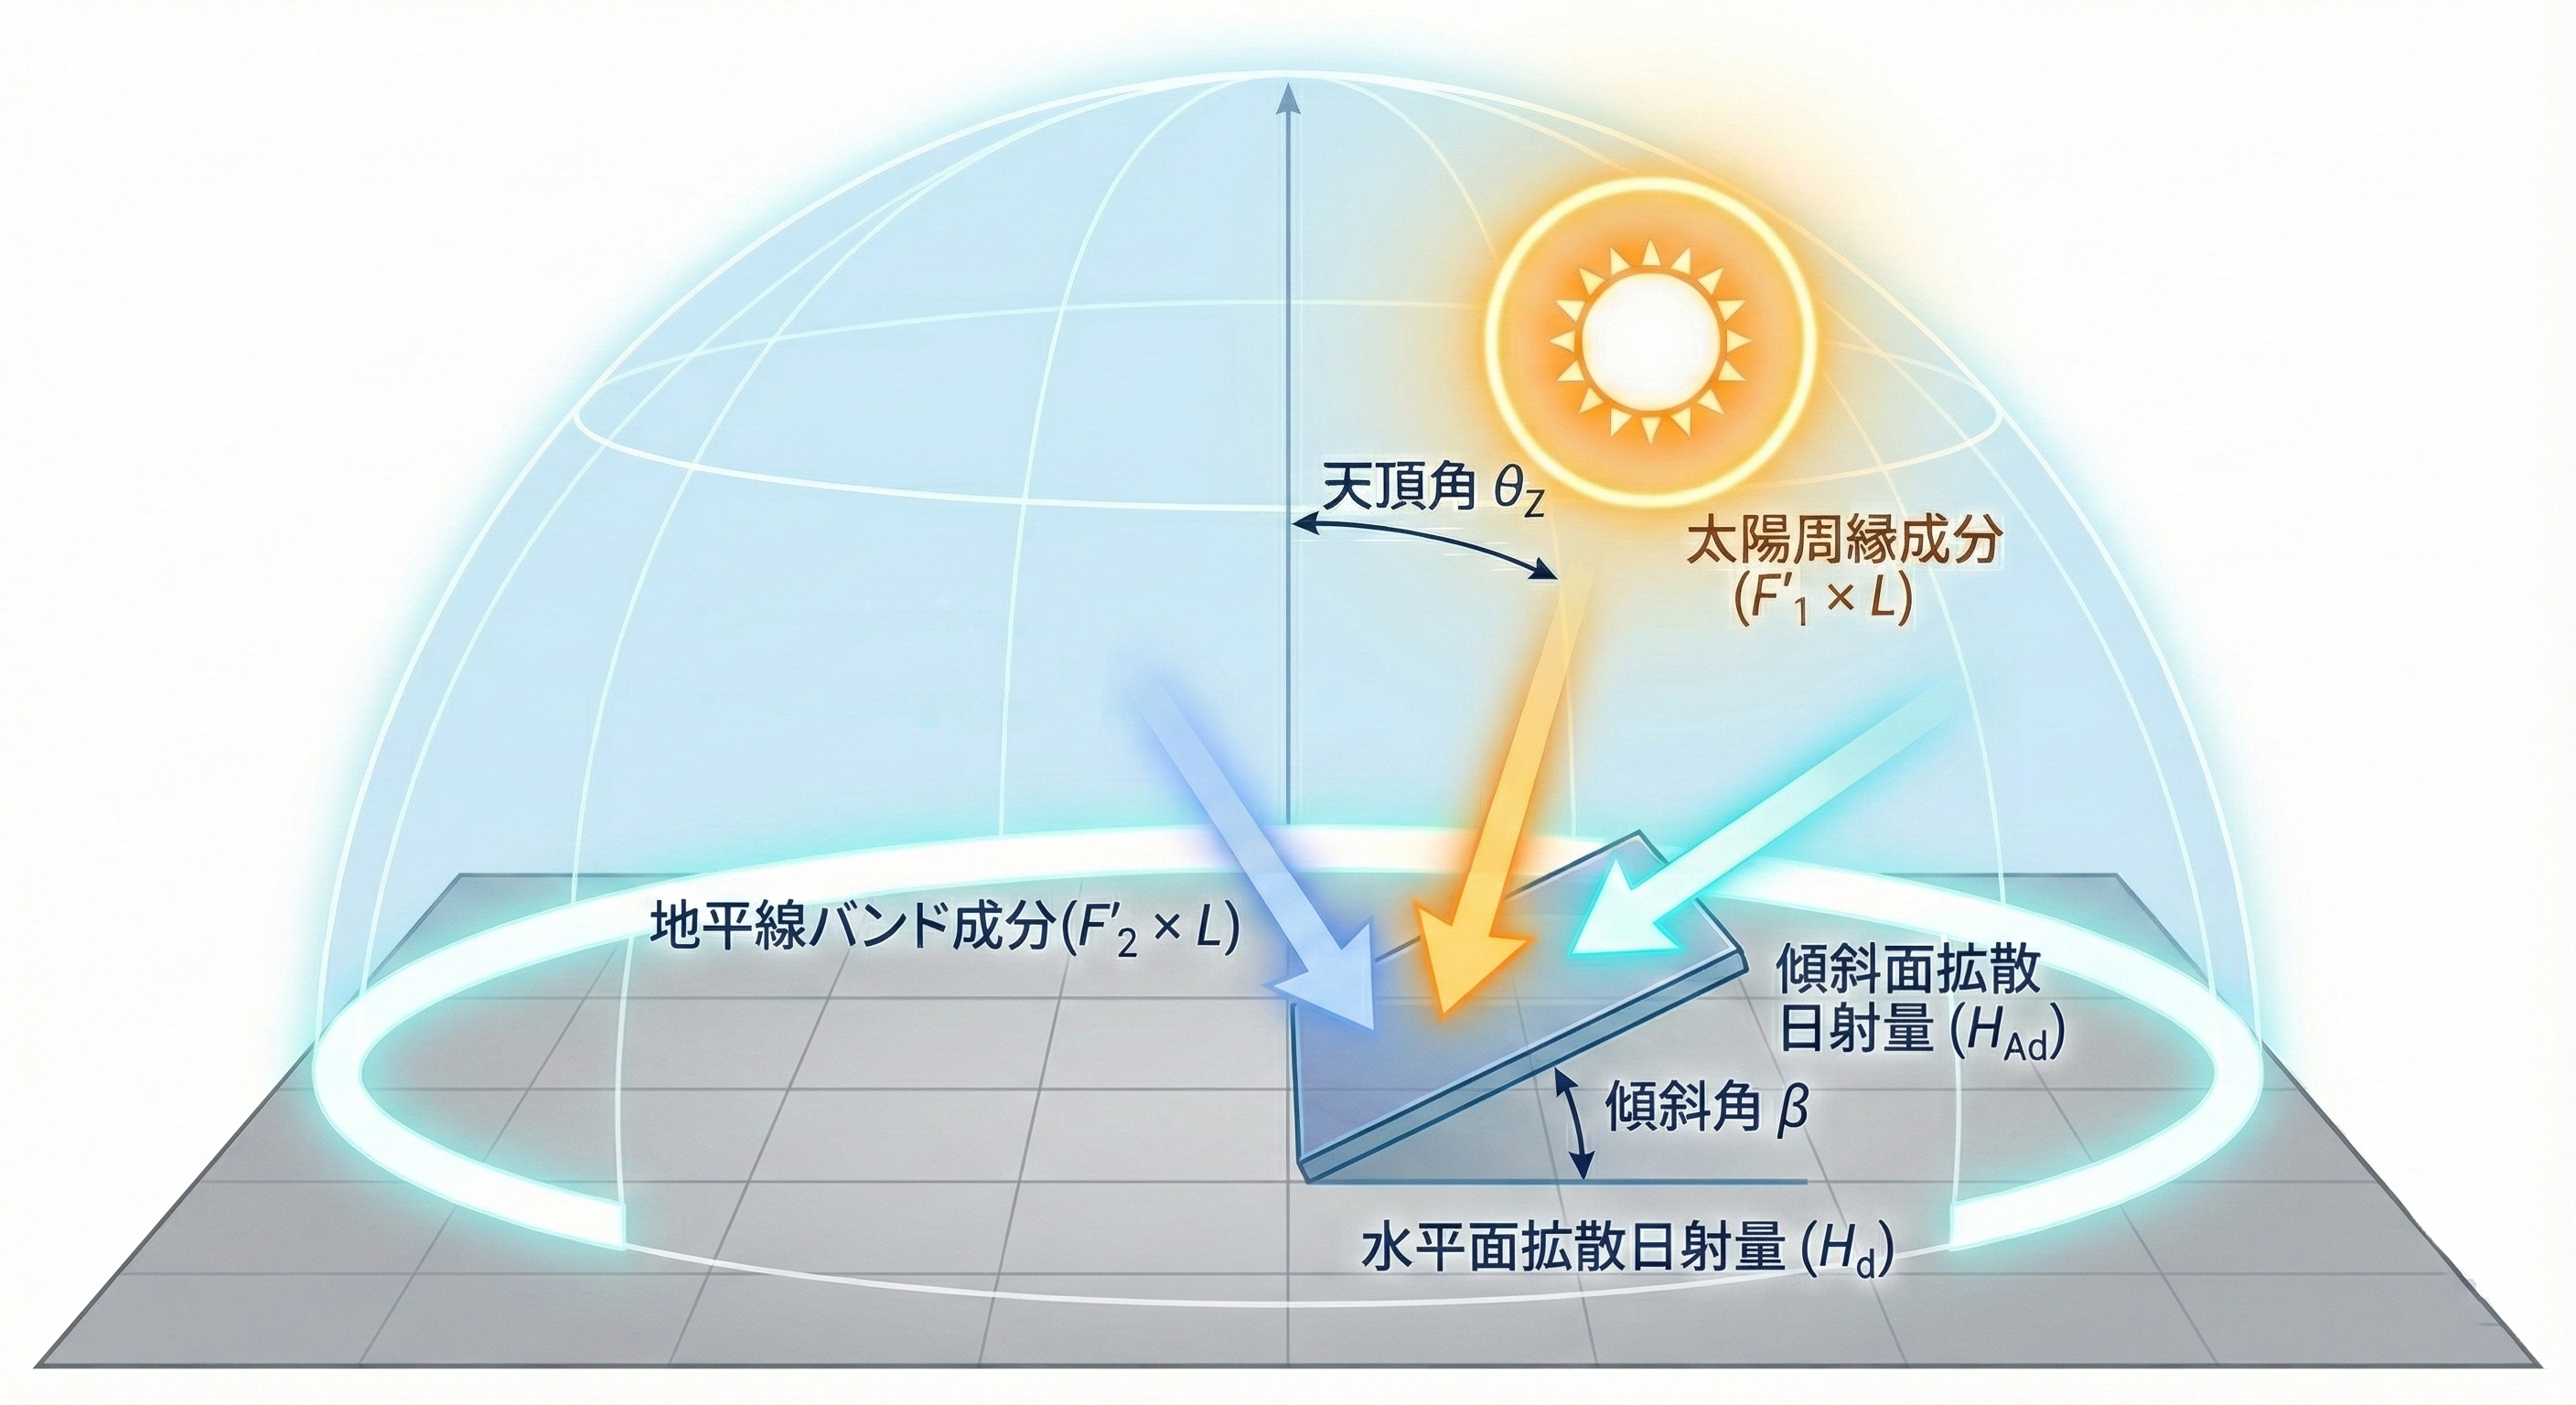
\includegraphics[width=1.0\textwidth]{foto/Perez.png}
    \caption{Perezモデルの概念図}
    \label{fig:Perez}
\end{figure}
\FloatBarrier

Perez モデルは、天空日射の散乱成分を「全天空一様な強さの散乱光($L$)」、「太陽周辺光($F'_1 \times L$, 視半径 $\alpha = 25 [\text{deg.}]$)」、および「地平線光($F'_2 \times L$, $\xi \sim 0$)」の3成分の和として表現するモデルである。
ここで、$F'_1$ および $F'_2$ は入射光の状態(天頂角 $\theta_Z$、水平面散乱日射量 $H_d$、晴天度パラメータ $\epsilon$)に依存する係数であり、これらを用いることで、天空の状態を水平面全天日射量 $H_g$、水平面散乱日射量 $H_d$、および直達日射量 $H_b$ だけで表現することが可能となる。係数 $F'_1, F'_2$ の算出式を式(\ref{eq:perez_f1})に示す。

\begin{equation}
\begin{split}
    F'_1 &= F'_{11}(\epsilon) + F'_{12}(\epsilon) \cdot \Delta + F'_{13}(\epsilon) \cdot \theta_Z \\
    F'_2 &= F'_{21}(\epsilon) + F'_{22}(\epsilon) \cdot \Delta + F'_{23}(\epsilon) \cdot \theta_Z
\end{split}
\label{eq:perez_f1}
\end{equation}

ここで、$\Delta$ は散乱光パラメータ、$\epsilon$ は晴天度パラメータの算出式をそれぞれ式(\ref{eq:perez_epsilon})、式(\ref{eq:perez_AM_A})に示す。

\begin{equation}
    \epsilon = \frac{H_d + H_b}{H_d}
\label{eq:perez_epsilon}
\end{equation}

\begin{equation}
    \Delta = AM_A \cdot \frac{H_d}{H_0}
\label{eq:perez_AM_A}
\end{equation}

また、$F'_{11}(\epsilon), F'_{12}(\epsilon), \dots, F'_{23}(\epsilon)$ は晴天度 $\epsilon$ に依存する係数であり、表\ref{tab:perez_coeffs}に対応する値を用いる。これらの値は、フランスのTrappesおよびCarpentrasにおける5つの傾斜面の時積算全天日射量の3年分のデータを用いて導出されたものである。

\begin{table}[hbt]
    \centering
    \caption{Perezモデルのパラメータ}
    \label{tab:perez_coeffs}
    \renewcommand{\arraystretch}{1.3} % 增加行高,防止数字太挤
    \small
    \begin{tabular}{c|rrrrrr}
        \hline
        $\epsilon$ & $F'_{11}(\epsilon)$ & $F'_{12}(\epsilon)$ & $F'_{13}(\epsilon)$ & $F'_{21}(\epsilon)$ & $F'_{22}(\epsilon)$ & $F'_{23}(\epsilon)$ \\
        \hline
        $\epsilon \le 1.056$          & $-0.011$ & $0.748$  & $-0.080$ & $-0.048$ & $0.073$  & $-0.024$ \\
        $1.056 < \epsilon \le 1.253$  & $-0.038$ & $1.115$  & $-0.109$ & $-0.023$ & $0.106$  & $-0.037$ \\
        $1.253 < \epsilon \le 1.586$  & $0.166$  & $0.909$  & $-0.179$ & $0.062$  & $-0.021$ & $-0.050$ \\
        $1.586 < \epsilon \le 2.134$  & $0.419$  & $0.646$  & $-0.262$ & $0.140$  & $-0.167$ & $-0.042$ \\
        $2.134 < \epsilon \le 3.230$  & $0.710$  & $0.025$  & $-0.290$ & $0.243$  & $-0.511$ & $-0.004$ \\
        $3.230 < \epsilon \le 5.980$  & $0.857$  & $-0.370$ & $-0.279$ & $0.267$  & $-0.792$ & $0.076$ \\
        $5.980 < \epsilon \le 10.080$ & $0.734$  & $-0.073$ & $-0.228$ & $0.231$  & $-1.180$ & $0.199$ \\
        $10.080 < \epsilon$           & $0.421$  & $-0.661$ & $0.097$  & $0.119$  & $-2.125$ & $0.446$ \\
        \hline
    \end{tabular}
\end{table}
\FloatBarrier

以上の係数を用いた,傾斜面散乱日射量$H_{Ad}$の推定式を定義する。

\begin{equation}
    H_{Ad} = H_d \left[ 0.5 \cdot (1 + \cos\beta) \cdot (1 - F'_1) + F'_1 \cdot \left( \frac{\chi_c}{\chi_h} \right) + F'_2 \cdot \sin\beta \right]
\end{equation}

ここで$\chi_c$および$\chi_h$はそれぞれ式(\ref{eq:perez_chi_c})および式(\ref{eq:perez_chi_h})で求まる。

\begin{equation}
    \chi_c = 
    \begin{cases}
        \psi_h \cdot \cos\theta & (\theta < \frac{\pi}{2} - \alpha) \\
        \psi_h \cdot \psi_c \cdot \sin(\psi_c \cdot \alpha) & (\frac{\pi}{2} - \alpha \le \theta \le \frac{\pi}{2} + \alpha) \\
        0 & (\frac{\pi}{2} + \alpha < \theta)
    \end{cases}
    \label{eq:perez_chi_c}
\end{equation}

\begin{equation}
    \chi_h = 
    \begin{cases}
        \cos\theta_Z & (\theta_Z < \frac{\pi}{2} - \alpha) \\
        \psi_h \cdot \sin(\psi_c \cdot \alpha) & (\frac{\pi}{2} - \alpha \le \theta_Z)
    \end{cases}
    \label{eq:perez_chi_h}
\end{equation}

ただし$\theta$は入射角[rad.],$\theta_Z$は天頂角[rad.],$\alpha$は太陽の視半径($= 0.436[\text{rad.}]$)である。また$\psi_c$および$\psi_h$はそれぞれ太陽周辺光部分が斜面で隠れない割合と水平線上に出ている割合相当するものであり,次のように表される。

\begin{equation}
    \psi_c = \frac{\frac{\pi}{2} - \theta + \alpha}{2\alpha}
\end{equation}

\begin{equation}
    \psi_h = 
    \begin{cases}
        1 & (\theta_Z < \frac{\pi}{2} - \alpha) \\
        \dfrac{\frac{\pi}{2} - \theta_Z + \alpha}{2\alpha} & (\frac{\pi}{2} - \alpha \le \theta_Z)
    \end{cases}
\end{equation}

%------------------------------------------------------------------------
\subsection{傾斜面直達日射量\texorpdfstring{$H_{Ab}$}{H\_Ab}推定}
\label{sec:傾斜面直達日射量推定} 
%------------------------------------------------------------------------

本項では直達日射量$H_b$を用いて,傾斜面に入射する直達成分(傾斜面直達日射量$H_{Ab}$)を推定する。

\begin{equation}
    H_{Ab} = H_b \cdot \cos \theta
\end{equation}

ここで$\theta$は PV システムへの日射入射角[rad.]である。

%------------------------------------------------------------------------
\subsection{傾斜面反射日射量\texorpdfstring{$H_{Ar}$}{H\_Ar}推定}
\label{sec:傾斜面反射日射量推定} 
%------------------------------------------------------------------------

本項では測定水平面全天日射量$H_g$と地表の反射度を表す地表面アルベド$\rho$, PV システムの設置傾斜角$\beta [\text{rad.}]$を用いて, 傾斜面に入射する地表面からの反射成分(傾斜面反射日射量$H_{Ar}$)を推定する。推定するにあたって, 地表面における日射の反射は全方位に対して一様であると仮定している(均一反射モデル)。

\begin{equation}
H_{Ar} = \rho \cdot H_g \cdot \frac{1 - \cos \beta}{2} \tag{4-27}
\end{equation}

ここで地表面アルベドは地表の状態で変化するが, 各状態での推定は困難であるため本論文中では ISO や JIS 等の基準スペクトルの際に用いられている 0.2 で固定している。

%------------------------------------------------------------------------
\subsection{傾斜面日射量\texorpdfstring{$H_{Ag}$}{H\_Ag}推定}
\label{sec:傾斜面日射量推定} 
%------------------------------------------------------------------------

以上 傾斜面散乱日射量$H_{Ad}$、傾斜面直達日射量$H_{Ab}$と傾斜面反射日射量$H_{Ar}$にて求められた日射の各成分を足し合わせて, 傾斜面日射量$H_{Ag}$の推定値とする。

\begin{equation}
H_{Ag} = H_{Ad} + H_{Ab} + H_{Ar} \tag{4-28}
\end{equation}

%************************************************************************
\section{システムその他損失係数の導出}
\label{sec:システムその他損失係数の導出} 
%************************************************************************

本節では、各太陽光発電システム(リファレンスシステム)固有の性能特性を定量化するための指標である「その他損失係数($K_O(t)$)」の定義および導出プロセスについて述べる。本手法において$K_O(t)$は、温度損失以外のすべての損失(配線損失、汚れ、経年劣化、影の影響など)を包括するパラメータとして位置づけられる損失係数を定義し、その導出プロセスについて述べる。本手法の特徴は、損失係数を定数として扱うのではなく、各システムの稼働年数、季節、および時間帯ごとの変動を捉える動的なパラメータとしてモデル化する点にある。

%------------------------------------------------------------------------
\subsection{学習用データの選別}
\label{sec:学習用データの選別} 
%------------------------------------------------------------------------

システム固有のその他損失係数($K_O(t)$)を正確に算出するためには、気象観測地点と発電システム地点が天気状態が一致な「晴天日」のデータを抽出する必要がある。本手法の構築における最大の制約は、発電所現地に日射計が設置されていない点にある。そのため、代替として気象庁のアメダス等の遠隔地点で観測された水平面全天日射量($GHI$)データを使用せざるを得ないが、観測地点と発電所間の地理的距離(数\,km-数十\,km)に起因する天候の非一致性が課題となる。局所的な気象変化により、観測地点が晴天であっても発電所上空のみに雲がかかっている場合、遠隔地の $GHI$ をそのまま適用すると、発電電力の低下が設備の不具合によるものか、あるいは単なる日陰によるものかを判別できず、データの信頼性が著しく低下する。この過程は\ref{fig:simirarity}に示す。

この課題を解決するため、本研究では $GHI$ と対象システムの発電電力($P_{DC}$)の時系列波形の類似性に着目し、コサイン類似度(Cosine Similarity)を用いたフィルタリング手法を採用した。理想的な晴天日において、$GHI$ と $P_{DC}$ はともに太陽の高度角の変化に従い、滑らかな「ベル型」の波形を描く。観測地点と発電所が離れていても、広域的に快晴である日は両地点で同様の滑らかな波形が観測されるため、形が高度に一致する日のみを選別することで、遠隔地の気象データを現地の正解的な気象データとして代用する際の妥当性を確保できる。

具体的には、ある日における日の出から日の入りまでのデータベクトルをそれぞれ $\vec{P_{DC}}$、$\vec{GHI}$ としたとき、その類似度 $Similarity$ は次式で定義される。

\begin{equation}
    Similarity = \frac{\vec{P_{DC}} \cdot \vec{GHI}}{|\vec{P_{DC}}| |\vec{GHI}|} = \frac{\sum_{t=1}^{N} (P_{DC}(t) \times GHI(t))}{\sqrt{\sum_{t=1}^{N} (P_{DC}(t))^2} \times \sqrt{\sum_{t=1}^{N} (GHI(t))^2}}
\end{equation}

ここで、$N$ は1日のデータ点数である。$Similarity$ は波形の「形状の一致度」を表す指標であり、値が1に近いほど両者の時間的挙動が一致していることを意味する。コサイン類似度はベクトルの絶対値ではなく向き(形状)を評価する指標であるため、受光特性や次元が異なる二つの物理量を比較する上で極めて有効である。

本研究では、予備解析の結果に基づき、$Similarity > 0.97$ という厳格な基準を満たす日のみを「有効な学習用データ」として選定した。この処理により、雲による不規則な変動を入り口で遮断し、配線損失やパネル劣化といったシステム内部のパラメータである $K_O(t)$ のみを純粋に算出できる状態を構築している。このように厳格な閾値によって遠隔地と現地の天候がわずかに異なる日を自動的に棄却することで、次項で述べるパラメータ導出および $K_O(t)$ マトリクス構築の精度を担保している。

\begin{figure}[htbp]
    \centering
    \includegraphics[width=1.0\textwidth]{foto/simirarity.png}
    \caption{コサイン類似度による晴天日データの選別イメージ}
    \label{fig:simirarity}
\end{figure}
\FloatBarrier

%------------------------------------------------------------------------
\subsection{理論発電量の定義と損失係数の概念}
\label{sec:理論発電量の定義と損失係数の概念}
%------------------------------------------------------------------------

PVシステムの発電電力 $P_{DC}(t)$ [W] は、傾斜面日射量 $H_{Ag}$ [W/m$^2$] およびモジュール温度 $T_c(t)$ [$^\circ$C] を用いて、以下の物理モデルにより表される。

\begin{equation}
    P_{DC}(t) = K_O \times \frac{H_{Ag}}{G_{STC}} \times [1 + \gamma(T_c(t) - T_{STC})] \times P_{STC}^{tot}
\end{equation}

ここで、各変数の定義は以下の通りである。

\begin{itemize}
    \item $G_{STC}$: 標準試験条件 (STC) における水平面日射量 (= 1000 W/m$^2$)
    \item $T_{STC}$: STCにおけるモジュール温度 (= 25 $^\circ$C)
    \item $P_{STC}^{tot}$: システムの定格容量 [W]
    \item $\gamma$: モジュールの出力温度係数 [\%/$^\circ$C] 
\end{itemize}

この式を変形することにより、ある時刻 $t$ における瞬時的なその他損失係数 $K_O(t)$ は、実測された発電電力と、気象データから計算される理論的なパラメータを用いて次式で算出される。

\begin{equation}
    K_O(t) = \frac{P_{DC}(t)}{\frac{H_{Ag}}{G_{STC}} \times [1 + \gamma(T_c(t) - T_{STC})] \times P_{STC}^{tot}}
\end{equation}

なお、計算に用いる傾斜面日射量 $H_{Ag}$ は、気象庁等の水平面全天日射量 ($GHI$) から、Erbsモデルによる直散分離およびPérezモデルによる斜面変換を経て算出された値を用いる(算出過程は2.1節参照)。

%------------------------------------------------------------------------
\subsection{統計的アプローチによる\texorpdfstring{$K_O(t)$}{K\_O(t)}マトリクスの構築}
\label{sec:統計的アプローチによる\texorpdfstring{$K_O(t)$}{K\_O(t)}マトリクスの構築}
%------------------------------------------------------------------------

前項で算出された瞬時的なその他損失係数 $K_O(t)$ は、センサーの測定ノイズや、晴天判定をすり抜けた微小な雲の通過などにより、確率的な変動を含んでいる。また、建物や樹木などの障害物による影の影響は、太陽の方位角および高度角に依存するため、季節 (月) と時間帯 (時刻) によって体系的に変化する特性を持つ。加えて、システムの経年劣化は年単位のタイムスケールで進行する。したがって、単一の固定値を採用するのではなく、これらの時間的・空間的な変動特性を反映可能な多次元モデルが必要となる。本研究では、前処理工程において抽出された「晴天日データ」のみを用い、以下の手順で統計的に $K_O(t)$ を決定した。

\vspace{1em} % 段落间增加一点垂直间距

\textbf{(1) 時空間グリッドによるデータの構造化} 

各PVシステムについて、季節変動と日周変動を捉えるため、「月」および「時間 (5時から19時まで)」を軸とする2次元グリッド ($12 \times 14$ のマトリクス) を定義した。過去の観測期間 (トレーニング期間) における全ての晴天日データを対象に、算出された $K_O(t)$ を対応するグリッドセル $(m, h)$ に蓄積した。これにより、連続的な時系列データを、太陽位置に依存する離散的な状態空間へとマッピングした。

\textbf{(2) 中央値 (Median) による代表値の決定} 

蓄積されたデータ群から、各グリッドの代表値 $K_O^{Grid}(m, h)$ を決定するにあたり、算術平均ではなく中央値 (Median) を採用した。これは、突発的な影や瞬間的な発電低下といった「外れ値」に対するロバスト性を確保するためである。正規分布に従わないノイズ成分が含まれる実フィールドデータにおいて、中央値は平均値よりも安定した推定が可能となる。

\begin{equation}
    K_O^{Grid}(m, h) = \underset{d \in \mathcal{D}_m}{\mathrm{median}} \left( K_O(d, h) \right)
    \label{eq:$K_O(t)$_grid_median}
\end{equation}

\begin{itemize}
    \item $\mathcal{D}_m$: 対象月 m において、前処理により選別された「晴天日」の集合を表す。
    \item $K_O(d, h)$: その月の日 d における時刻 h のその他損失係数を意味する。
\end{itemize}

この統計的処理により、一時的な気象ノイズを除去しつつ、特定の季節・時間帯に定常的に発生する構造的な影の影響や、システム固有の性能特性のみをパラメータとして抽出・学習することが可能となる。

%------------------------------------------------------------------------
\subsection{経年劣化傾向の線形近似}
\label{sec:経年劣化傾向の線形近似}
%------------------------------------------------------------------------

さらに、長期間(本研究では5年間)のデータ解析において、太陽光パネルの経年劣化(Degradation) を考慮する必要がある。各年の $K_O(t)$ の代表値をプロットすると、経年に伴う緩やかな低下傾向が確認できる。
そこで、過去の実績データに対して線形回帰分析を行い、検証対象年における $K_O(t)$ の値を線形外挿 (Linear Extrapolation) によって推定した。最終的な検証フェーズ(逆推定)においては、この季節・時間変動および経年劣化トレンドを反映した $K_O^{\mathrm{Test}}$ マトリクスを使用する。
%------------------------------------------------------------------------
\section{PV発電量の推定モデル}
\label{sec:PV発電量の推定モデル}
%------------------------------------------------------------------------

本節では、既知の発電電力$P_{\mathrm{DC}}$を入力情報として、未観測の全天日射量$GHI$を導出するための推定アルゴリズムの詳細について述べる。本研究の推定モデルは、物理的なエネルギー収支に基づく「逆推定モデル」と、PCSの非線形特性が顕著となる低照度領域を補間するための「データ駆動型アプローチ」を組み合わせたハイブリッド構造を有している。

%------------------------------------------------------------------------
\subsection{物理モデルに基づく日射量の探索的逆算}
\label{sec:物理モデルに基づく日射量の探索的逆算}
%------------------------------------------------------------------------

検証対象期間における任意の時刻 $t$ において、PCSに入力される発電電力 $P_{\mathrm{DC}}(t)$ と傾斜面日射量 $H_{Ag}$ の関係は、次式に示す物理モデルによって記述される。

\begin{equation}
    P_{\mathrm{DC}}(t) = K_{0}^{\mathrm{Test}} \times \frac{H_{Ag}(t)}{G_{\mathrm{STC}}} \times \left[ 1 + \gamma (T_{\mathrm{c}}(t) - T_{\mathrm{STC}}) \right] \times P_{\mathrm{STC}}^{\mathrm{tot}}
    \label{eq:p_dc_model}
\end{equation}

ここで、$K_O^{\mathrm{Test}}$ は、\ref{sec:統計的アプローチによる\texorpdfstring{$K_O(t)$}{K\_O(t)}マトリクスの構築}項で述べた過去5年間の稼働実績に基づく線形回帰分析から外挿された、検証対象年におけるシステム性能指数である。この $K_O^{\mathrm{Test}}$ を用いることで、経年劣化等のシステム個体差を適切に補正した状態での解析が可能となる。

本研究の目的は $P_{\mathrm{DC}}$ から $GHI$ を得ることにあるが、$H_{Ag}$ の算出プロセスには、全天日射量から直達・散乱成分を分離するErbsモデルや、周囲の空の輝度分布を考慮して斜面強度へ変換するPérezモデルといった複数の非線形な経験式が含まれる。そのため、$GHI$ について式(\ref{eq:p_dc_model})を直接的な代数計算によって解くことは困難である。

この問題に対し、本研究では「探索的逆算手法」を適用する。具体的には、$GHI$ の候補値を微小ステップで変化させながら逐次的に $P_{\mathrm{DC}}$ の理論値を計算し、実測された $P_{\mathrm{DC}}$ との誤差が最小となる $GHI$ を探索する。このアルゴリズムにより、日射計が未設置のサイトであっても、物理的な整合性を維持した形での日射量推定が実現される。

%------------------------------------------------------------------------
\subsection{変換効率の非線形性を考慮したハイブリッド推論}
\label{sec:変換効率の非線形性を考慮したハイブリッド推論}
%------------------------------------------------------------------------

前項の物理モデルは、PCSの変換効率が定格付近で一定と見なせる中・高出力領域においては極めて高い信頼性を示す。しかし、日出・日没前後や重い雲に覆われた状況などの低照度領域においては、推定精度の低下が顕著となる。これは、PCS内部の自己消費電力やスイッチング損失が相対的に増大し、入力電力に対する出力特性が非線形な立ち上がり特性を示すためである。特に、日出・日没時の極低照度時においては、太陽電池パネルが開放電圧($V_{\mathrm{oc}}$)に近い電圧を発生しているものの、PCSの起動電力に満たないために出力電力 $P_{\mathrm{DC}}$ がゼロとなる「不感帯」が存在する。物理モデルのみに依存した場合、出力がゼロであれば日射量もゼロと推定されるが、実際には微弱な日射が存在しており、この乖離が推定誤差の要因となる。

この物理的な限界を克服するため、本研究で物理モデルとデータ駆動型モデルを組み合わせたハイブリッド推論モデルを構築した。出力域($P_{\mathrm{DC}} > 0\,\mathrm{W}$)では物理モデルを優先的に適用し、システムの熱力学的特性に基づいた高精度な逆推定を行う一方、低照度域($P_{\mathrm{DC}} \leq 0\,\mathrm{W}$)においては、出力電圧 $V_{\mathrm{DC}}$ と出力電力 $P_{\mathrm{DC}}$ を特徴量とした機械学習モデル(ランダムフォレスト等)を併用する。

低照度域において電圧情報を活用する理論的根拠は、太陽電池の出力特性($I$-$V$ 特性)に由来する。太陽電池の開放電圧は水平面日射量の対数に比例して上昇するため、電流がほとんど流れない極低照度時であっても、電圧値には水平面日射量の変化が感度良く反映される。この特性を利用し、過去の膨大な学習データから「電圧・電力・時間の相関関係」を機械学習によりモデル化することで、物理モデルでは捉えきれないPCSの起動境界付近の日射量を精度良く推定することが可能となる。この手法により、PCSの動作点や非線形な変換効率に左右されることなく、日出から日没までの全時間帯において、連続的かつ安定した $GHI$ の推定精度を確保している。

%************************************************************************
\section{システム相互比較のメカニズム}
\label{sec:システム相互比較のメカニズム}
%************************************************************************

各システムから個別に逆推定された日射量の信頼性を客観的に評価するため、以下の3つの独立した評価指標を定義する。

\begin{enumerate}
    \item \textbf{正規化発電量とGHI推定値の一貫性指標 ($S_{\mathrm{consistency}}$)}

    この指標は、入力データである実測発電電力($P_{\mathrm{DC}}$)の波形と、物理モデルから逆推定された日射量($GHI$)の波形の整合性を評価するものである。
    \begin{equation}
        S_{\mathrm{consistency}} \propto \frac{1}{\mathrm{RMSE}(P_{\mathrm{DC}} - GHI)}
    \end{equation}

    \textbf{データ活用と計算プロセス:}
    解析対象日の日の出から日没までの時系列データ(1時間間隔、24点ベクトル)を使用する。まず、$P_{\mathrm{DC}}$ をその日の最大値で正規化し、同様に逆推定された $GHI$ カーブと比較を行う。物理モデルが正しく機能している場合、両者の波形は高度に一致する。雲の急変やモデルの不適合によって $\mathrm{RMSE}$(二乗平均平方根誤差)が増大した場合、分母が大きくなるためスコアは低下する。これにより、物理的につじつまの合わない推定結果を排除する。

    \item \textbf{データの品質指標 ($S_{\mathrm{quality}}$)}

    データの連続性および欠損状況を評価する指標である。
    \begin{equation}
        S_{\mathrm{quality}} \propto 1 - \mathrm{Ratio}_{\mathrm{NaN}}
    \end{equation}

    \textbf{データ活用と計算プロセス:}
    当該日における全データ点数に対する欠損値(NaN)の割合($\mathrm{Ratio}_{\mathrm{NaN}}$)を算出する。通信障害やセンサーエラーによってデータが一部欠落しているシステムは、日射量の推定カーブを正確に描画できないため、この指標によって評価を低減させる。すべてのデータが揃っている状態を $1.0$ とし、欠損が増えるに従って線形にスコアが減少する。

    \item \textbf{システムの安定性指標 ($S_{\mathrm{stability}}$)}

    対象システムの長期的な稼働状況の安定性を評価する指標である。
    \begin{equation}
        S_{\mathrm{stability}} \propto \frac{1}{\sigma (P_{\mathrm{DC\_day\_mean}}^{\mathrm{2month}})}
    \end{equation}

    \textbf{データ活用と計算プロセス:}
    この指標の計算には、推定対象日だけでなく、その月および前月の計2ヶ月間にわたる長期的な稼働データを使用する。まず、日ごとの平均発電電力($P_{\mathrm{DC\_day\_mean}}$)を算出し、その2ヶ月間の標準偏差($\sigma$)を求める。標準偏差が小さいことは、そのシステムが突発的な故障や樹木等の影の影響を恒常的に受けておらず、リファレンスとして安定していることを意味する。
\end{enumerate}

%------------------------------------------------------------------------
\subsection{システムの品質評価指標の定義}
\label{sec:システムの品質評価指標の定義}
%------------------------------------------------------------------------

前項で定義した3つの指標($S_{\mathrm{consistency}}, S_{\mathrm{quality}}, S_{\mathrm{stability}}$)を、それぞれ $0.0$ から $1.0$ の範囲で正規化した後、以下の重み付け係数を用いて統合し、各システムの総合的な「品質スコア($\mathrm{Quality}$)」を算出する。

\begin{equation}
\label{equation:システムの品質評価指標の定義}
    \mathrm{Quality} = 0.2 \cdot S_{\mathrm{consistency}} + 0.2 \cdot S_{\mathrm{quality}} + 0.6 \cdot S_{\mathrm{stability}}
\end{equation}

\textbf{統合の論理とデータ構造の適用:}
本手法では、長期的な稼働安定性を示す $S_{\mathrm{stability}}$ に対して $0.6$ という最大の重みを割り当てている。これは、日々の気象変化と発電量変化の一貫性やデータの品質よりも、システム自体が健全な状態にあるかどうかが、日射量推定の基準点として最も重要であるという知見に基づいている。

計算プロセスにおいては、サイト内の全システムに対して、個別にこの $\mathrm{Quality}$ スコアを毎時算出する。これにより、ある特定の時刻において、どのシステムの推定値がサイト全体の代表値として最も相応しいかを動的に判断する準備が整う。

%------------------------------------------------------------------------
\section{GHI推定精度評価指標}
\label{sec:GHI推定精度評価指標}
%------------------------------------------------------------------------

本研究で構築したハイブリッド推論モデルおよび複数システム合成アルゴリズムの有効性を定量的に評価するため、複数の精度評価指標を導入する。評価にあたっては、気象庁(アメダス)等で観測された水平面全天日射量の実測値($GHI_{\mathrm{meas}}$)を「正解」とし、提案手法による推定値($GHI_{\mathrm{est}}$)との乖離を以下の指標を用いて算出する。

%------------------------------------------------------------------------
\subsection{代表的な誤差指標の定義}
\label{sec:代表的な誤差指標の定義}
%------------------------------------------------------------------------

推定精度を多角的に評価するため、平均的な誤差の大きさ、偏差、およびバイアスの傾向を示す以下の4つの指標を主に使用する。

\begin{enumerate}
    \item \textbf{平均絶対誤差 (Mean Absolute Error: MAE)}

    各時刻における推定値と実測値の差の絶対値を平均したものであり、直感的な精度の尺度となる。
    \begin{equation}
        \mathrm{MAE} = \frac{1}{n} \sum_{i=1}^{n} |GHI_{\mathrm{est},i} - GHI_{\mathrm{meas},i}| \quad [\mathrm{W/m^2}]
    \end{equation}

    \item \textbf{二乗平均平方根誤差 (Root Mean Square Error: RMSE)}

    誤差の二乗を平均して平方根をとったものであり、大きな誤差(外れ値)に対して敏感に反応する特性を持つ。物理モデルの不適合や突発的なノイズを検出する上で重要な指標である。
    \begin{equation}
        \mathrm{RMSE} = \sqrt{\frac{1}{n} \sum_{i=1}^{n} (GHI_{\mathrm{est},i} - GHI_{\mathrm{meas},i})^2} \quad [\mathrm{W/m^2}]
    \end{equation}

    \item \textbf{正規化二乗平均平方根誤差 (Normalized RMSE: nRMSE)}

    RMSE を実測値の平均値 $\overline{GHI_{\mathrm{meas}}}$ で除して百分率で表したものである。水平面日射量の異なる季節間や地域間での精度比較を可能にする。
    \begin{equation}
        \mathrm{nRMSE} = \frac{\mathrm{RMSE}}{\overline{GHI_{\mathrm{meas}}}} \times 100 \quad [\%]
    \end{equation}

    \item \textbf{平均バイアス誤差 (Mean Bias Error: MBE)}

    推定値の平均的な過大・過小評価の傾向を示す。物理モデルにおける損失係数 $K_0$ の設定妥当性や、系統的な誤差(ドリフト)の有無を判定するために用いる。
    \begin{equation}
        \mathrm{MBE} = \frac{1}{n} \sum_{i=1}^{n} (GHI_{\mathrm{est},i} - GHI_{\mathrm{meas},i}) \quad [\mathrm{W/m^2}]
    \end{equation}
\end{enumerate}

%************************************************************************
\subsection{統計的相関と誤差パターンの分析手法}
\label{sec:統計的相関と誤差パターンの分析手法}
%************************************************************************

単一の数値指標に加え、推定モデルの挙動を詳細に把握するため、以下の分析アプローチを併用する。

\begin{itemize}
    \item \textbf{相関係数 ($R$) および決定係数 ($R^2$):}
    実測値と推定値の散布図における線形的な一致度を評価する。

    \item \textbf{時間的・季節的誤差推移の解析:}
    Python による多角的な誤差分析(Error Pattern Analysis)に基づき、時刻別および月別の誤差分布を算出する。

    \item \textbf{物理的整合性の検証:}
    推定された $GHI$ が物理的な上限(大気外日射量 $H_0$)を超えていないか、あるいは夜間や低照度時に負の値をとっていないかを確認し、インバージョンアルゴリズムの健全性を評価する。
\end{itemize}

以上の指標を用いることで、提案手法が実運用の監視システムにおいて、どの程度の信頼性を持って日射計の代替を果たし得るかを総合的に評価する。

%************************************************************************
\section{GHI推定値の選択と時系列合成}
\label{sec:GHI推定値の選択と時系列合成}
%************************************************************************

第\ref{sec:GHI推定値の選択と時系列合成}節では、第\ref{sec:システム相互比較のメカニズム}節において定義した品質スコアに基づき、複数の太陽光発電システムから得られる個別推定値を統合する手法について述べる。本手法の目的は、各サイトを代表する単一の全天日射量(GHI)時系列データを生成することにある。これにより、スパイクノイズや不連続点といった物理的な不整合を排除しつつ、実際の気象変化を忠実に再現した高精度な日射量曲線を得ることが可能となる。

%------------------------------------------------------------------------
\subsection{動的選択アルゴリズム}
\label{sec:動的選択アルゴリズム}
%------------------------------------------------------------------------

サイト内に設置された全てのシステムから得られる各時刻 $t$ の日射量推定値に対し、以下の手順で代表値を選定する。まず、当該時刻に稼働している全システムを対象に日射量の逆推定を実施する。次に、\ref{equation:システムの品質評価指標の定義}で算出した品質スコアに基づき、その時刻において最も信頼性が高いと判断されるシステムを動的に選択する。このアプローチにより、一部のシステムで局所的な遮蔽や一時的な通信障害が発生した場合でも、他の健全なシステムから得られた推定値を用いて自動的にデータを補完することができる。

%------------------------------------------------------------------------
\subsection{太陽高度角に応じた動的フィルタリング}
\label{sec:太陽高度角に応じた動的フィルタリング}
%------------------------------------------------------------------------

時系列データの合成過程において、物理的に不合理な異常スパイクを検出・除去するため、太陽高度角に連動した動的閾値を適用する。時間帯による日射特性の違いを考慮し、以下の基準でフィルタリングを行う。

\begin{itemize}
    \item \textbf{高高度角領域:} 水平面日射量が安定しやすい時間帯であるため、閾値を厳格に設定(例:$\pm 250$ W/m$^2$)し、微細な異常値についても徹底的な排除を図る。
    \item \textbf{低高度角領域:} 大気の影響や遮蔽物の影響を受けやすく、日射変動が大きくなりやすい性質を考慮し、閾値を緩和することで、急峻な天候変化に伴う自然な変動を許容する。
\end{itemize}

このように時間帯に応じた最適な帯域制限を設けることで、ノイズ除去を実現している。

%------------------------------------------------------------------------
\subsection{時系列合成と加重平滑化処理}
\label{sec:時系列合成と加重平滑化処理}
%------------------------------------------------------------------------

選別された推定値を連結するプロセスでは、接合部における段差を抑制し、データの連続性を担保するために以下の処理を施す。

\begin{enumerate}
    \item \textbf{異常値の修正:} 前述の動的閾値によって外れ値と判定されたデータ点は、前後の時系列データを用いた線形補間により修正を行う。
    \item \textbf{品質スコアに基づく加重移動平均:} 合成された曲線に対し、前後3点のデータを用いた移動ウインドウによる平滑化を行う。この際、単純な算術平均ではなく、算出された品質スコアを重みとして配分する。
\end{enumerate}

品質スコアが高いデータ点はその値を重視して維持し、逆にスコアが低い点は周囲の信頼性の高いデータと滑らかに馴染ませる処理を行う。本アルゴリズムの導入により、単一システムでは回避が困難な局所的誤差や欠損を空間的・時間的に補償することが可能となった。結果として、日射計が未設置のサイトにおいても、物理的整合性の取れた高精度な気象リファレンスを構築できる。

%************************************************************************
\section{定常日陰検出モデル}
\label{sec:定常日陰検出モデル}
%************************************************************************

本節では、太陽光発電システムの設置環境に起因する樹木や近隣構造物による定常的な日陰を自動検出し、その影響範囲を特定するアルゴリズムについて述べる。本モデルの導入により、システム特性 $K_0$ の同定精度の向上と、異常診断における信頼性の確保を図る。

%------------------------------------------------------------------------
\subsection{理論発電電力との比較による誤差抽出}
\label{sec:理論発電電力との比較による誤差抽出}
%------------------------------------------------------------------------

日陰の検出にあたっては、まず第\ref{sec:GHI推定値の選択と時系列合成}節で算出した合成GHIを入力値とし、対象システムの理論的な発電電力 $P_{model}(t)$ を以下の通り推定する。

\begin{equation}
P_{model}(t) = K_{0}^{Test} \times \frac{H_{Ag}(t)}{G_{STC}} \times [1 + \gamma (T_c(t) - T_{STC})] \times P_{STC}^{tot}
\end{equation}

ここで得られた理論値と、実際の計測値 $P_{meas}(t)$ との偏差を誤差 $\Delta P(t)$ と定義する。

\begin{equation}
\Delta P(t) = P_{meas}(t) - P_{model}(t)
\end{equation}

$\Delta P(t) < 0$ となる領域は、理論上の期待値に対して実際の出力が不足していることを示しており、これが日陰検出のための基礎データとなる。

\subsection{K-means法による誤差パターンのクラスタリング}

抽出された誤差には、雲の通過に伴う一時的な変動と、遮蔽物による定常的な出力低下が混在している。本研究では、これらを分離するために、以下の特徴量ベクトル $\vec{x}$ を用いたK-means法による非教師あり学習を実施する。

\begin{equation}
\vec{x} = [ \Delta P, \alpha, \phi, k_t, h, R_{res} ]^\top
\end{equation}

各変数は、太陽高度角 $\alpha$、太陽方位角 $\phi$、晴天指数 $CI$($GHI / H_0$)、時刻 $h$、および誤差率 $R_{res}$($|\Delta P| / P_{meas}$)を表す。クラスタ数を $k=3$ に設定し、各データ点を「正常運用」「軽微な日陰」「重度の日陰」の3つの状態に分類する。これにより、統計的な外れ値の影響を排除し、特定の気象条件や時間帯に共通して現れる日陰の強度を抽出する。

%------------------------------------------------------------------------
\subsection{SHAP分析を用いた日陰要因の空間的特定}
\label{sec:SHAP分析を用いた日陰要因の空間的特定}
%------------------------------------------------------------------------

クラスタリングによって特定された出力低下が、天候に起因するものか、あるいは太陽位置に依存するものかを判別するため、ランダムフォレストモデルを用いたSHAP(Shapley Additive Explanations)分析を導入する。SHAP値 $\phi_j$ は、モデルの予測値に対する各特徴量 $j$ の寄与度を表し、次式によって算出される。

\begin{equation}
\phi_j = \sum_{S \subseteq \{x_1, \dots, x_p\} \setminus \{x_j\}} \frac{|S|!(p - |S| - 1)!}{p!} [f(S \cup \{x_j\}) - f(S)]
\end{equation}

ここで $p$ は特徴量の総数、$f(S)$ は特徴量集合 $S$ を用いたモデルの予測値である。本解析において、方位角 $\phi$ および高度角 $\alpha$ のSHAP値が有意に高い場合、その出力低下は特定の太陽位置において発生していることを意味し、定常的な遮蔽物の存在を強く示唆する。

%------------------------------------------------------------------------
\subsection{方位・高度角マップによるマスク処理の実行}
\label{sec:方位・高度角マップによるマスク処理の実行}
%------------------------------------------------------------------------

最終的に、SHAP分析および角度別誤差解析の結果に基づき、方位角10$^\circ$、高度角5$^\circ$刻みの分解能でサイト内の日陰分布をマッピングする。

\begin{equation}
Mask(\phi, \alpha) =
\begin{cases}
1 & (\Delta P_{mean}(\phi, \alpha) < \text{Threshold}) \\
0 & (\text{otherwise})
\end{cases}
\end{equation}

このマスク値が1となる領域のデータは、第2.2節における損失係数 $K_0$ の学習プロセスから自動的に除外(スクリーニング)される。これにより、設置環境由来の不可避な出力低下が性能評価を歪めることを防ぎ、高精度な日射量推定モデルの構築が可能となる。

%========================================================================
% 第3章 解析地域と使用データ (Data Set)
%========================================================================
\chapter{解析地域と使用データ (Data Set)}
\label{chapter:解析地域と使用データ (Data Set)} 

本研究では、提案する日射量推定および異常診断手法の有効性を多角的に検証するため、設置環境および地理的特性の異なる2つのデータセットを使用する。

データセットAは、同一サイト内に多数のPVシステムが隣接して整然と配置された環境であり、手法の構築および複数システムの統合ロジックの最適化を目的とする。このデータセットでは、各パネル間の距離が極めて近く、逆推定される日射量はパネル群の直近の気象状態を正確に反映している。

データセットBは、広範囲に分散した屋根設置型のPVアレイ群であり、開発した手法の検証を目的とする。本地点では各システム間の距離が遠く、設置方位や傾斜角も個々に異なる。また、算出される推定値はアレイ群の中央領域を代表する地点のものであり、各パネル位置との間には一定の地理的距離が存在する。このような実環境に近い制約下での検証を通じて、手法の汎用性を評価する。

%************************************************************************
\section{データセットA:山梨県北杜サイト}
%************************************************************************

%------------------------------------------------------------------------
\subsection{解析対象地点の概要}
\label{sec:解析対象地点の概要}
%------------------------------------------------------------------------

本データセットは、山梨県北杜市長坂町に設置された太陽光発電所から取得したものである。山梨県北杜市長坂町の同一敷地内に集約して設置された太陽光発電施設から取得したものである。本地点では、2018年から2023年までの観測データを使用する。 

最大の特徴は、解析対象となる15系統のPVシステムが極めて狭い範囲に隣接して配置されている点にある。これにより、パネル間の気象条件の差異を最小限に抑えつつ、多数のシステムから信頼性の高いデータを自由に選択して分析に供することが可能である。

図\ref{fig:hokuto_aerial}に、本解析対象地点である山梨県北杜市の発電所の航空写真を示す。本地点は大規模な敷地内に多数のPVシステムが整然と集約して設置されており、高密度なシステム間比較に適した環境となっている。

地形は概ね平坦であるものの、図\ref{fig:hokuto_aerial}の南西方向には樹林が隣接している。この地理的要因により、太陽高度が低い冬期や夕方の時間帯において、樹林に近い特定のシステムでは定常的な日陰による発電量低下が確認されている。

\begin{figure}[htbp]
    \centering
    \includegraphics[width=0.9\linewidth]{foto/hokuto_aerial_view.jpg} 
    \caption{山梨県北杜市長坂町における解析対象発電所の航空写真}
    \label{fig:hokuto_aerial}
\end{figure}
\FloatBarrier  % <--- 强制在此之前的所有图片必须输出,不能漂到这里之后

%------------------------------------------------------------------------
\subsection{PVシステム構成と設備情報}
\label{sec:PVシステム構成と設備情報}
%------------------------------------------------------------------------

本解析の対象となる北杜サイト内のPVシステムは、単結晶シリコン系(5系統)および多結晶シリコン系(7系統)の計12系統で構成されている。表\ref{tab:hokuto_systems}に、各システムの設備構成一覧を示す。

\begin{table}[htbp]
    \centering
    \caption{北杜市サイトにおけるPVシステム設備構成一覧}
    \label{tab:hokuto_systems}
    \begin{tabular}{ccccccc}
        \hline
        ID & モジュール & セルタイプ & 定格容量 & 方位角 & 傾斜角 & 温度係数 $\beta_1$ \\
        (SiteAddress) & メーカー & (PVタイプ) & [kW] & [deg.] & [deg.] & [\%/$^\circ$C] \\ \hline
        19 & Sun Power & 単結晶 & 10.08 & 0 & 30.0 & -0.4 \\
        21 & Sun Power & 単結晶 & 10.08 & 0 & 30.0 & -0.4 \\
        28 & KPE & 単結晶 & 10.08 & 0 & 30.0 & -0.46 \\
        31 & Isofoton & 単結晶 & 11.20 & 0 & 30.0 & -0.46 \\
        34 & GE & 単結晶 & 10.38 & 0 & 30.0 & -0.46 \\ \hline
        44 & 京セラ & 多結晶 & 10.00 & 0 & 30.0 & -0.49 \\
        45 & 京セラ & 多結晶 & 10.00 & 0 & 30.0 & -0.49 \\
        46 & 京セラ & 多結晶 & 10.00 & 0 & 30.0 & -0.49 \\
        16 & シャープ & 多結晶 & 10.02 & 0 & 30.0 & -0.49 \\
        17 & シャープ & 多結晶 & 10.02 & 0 & 30.0 & -0.49 \\
        36 & Suntech & 多結晶 & 10.80 & 0 & 30.0 & -0.49 \\
        37 & Suntech & 多結晶 & 10.80 & 0 & 30.0 & -0.49 \\ \hline
    \end{tabular}
\end{table}
\FloatBarrier  % <--- 强制在此之前的所有图片必须输出,不能漂到这里之后

%------------------------------------------------------------------------
\subsection{計測データの特性と前処理}
\label{sec:計測データの特性と前処理}
%------------------------------------------------------------------------

現地では、PV出力電力およびモジュール温度が1分間隔の極めて高い時間粒度で記録されている。本研究では、気象庁データとの整合性を確保するため、これらの1分値を算術平均により1時間値へとダウンサンプリングして解析に供した。また、検証用の「正解」として、現地に設置された日射計(全天日射計)による実測水平面日射量データを使用する。

%************************************************************************
\section{データセットB:茨城県}
\label{sec:データセットB:茨城県}
%************************************************************************

本研究の汎用性を検証するため、茨城県内に点在する12箇所の太陽光発電システムを対象とする。これらの発電データは「福島県再生可能エネルギー導入促進支援事業」を通じて提供されたものである。

図\ref{fig:ibaraki_map}に、茨城県における各システムの地理的分布および気象庁・筑波観測点(AMeDAS)の位置関係を示す。本地点におけるシステムの詳細な位置情報、および筑波観測点との位置関係をインタラクティブに確認可能な地図データを、以下のリンクから参照できる。

\begin{figure}[H] 
    \centering
    % 点击图片也可以打开附件 (使用 textattachfile 包裹图片)
    \textattachfile[color=0 0 0]{foto/ibarakijyo_map.html}{
        \includegraphics[width=0.9\textwidth]{foto/Ibaraki_map.jpg}
    }
    
    \caption{茨城県における各PVシステムおよび筑波観測点の位置関係}
    \label{fig:ibaraki_map}
    
    % 注记区域
    \begin{quote}
        \footnotesize 

        注記:図をクリックするか、以下のリンクを選択することで、ファイルを保存してから詳細なインタラクティブマップ(HTML)をブラウザで閲覧可能である。\\

        \textbf{
            \textattachfile[color=0 0 0, mimetype=text/html]{foto/ibarakijyo_map.html}{
                [ \faExternalLink* \ 添付ファイルを開く:茨城県PVシステム分布図 (HTML) ]
            }
        }
    \end{quote}
\end{figure}

\FloatBarrier

%------------------------------------------------------------------------
\subsection{設備構成の詳細}
\label{sec:設備構成の詳細}
%------------------------------------------------------------------------

データセットBに含まれるシステムは、表\ref{tab:ibaraki_systems}に示す通り、設置容量が11.0 kWから44.0 kWまで多岐にわたり、モジュールタイプやパネルメーカーも非均一な構成となっている。また、屋根設置型であるため、方位角が東向き($-82^\circ$)から南西向き($62^\circ$)まで大きく異なり、データセットA(北杜市)と比較して、より実環境に近い複雑な条件下での解析を行う。

\begin{table}[htbp]
    \centering
    \caption{茨城県内におけるPVシステムの設備仕様一覧}
    \label{tab:ibaraki_systems}
    \begin{tabular}{ccccccc}
        \hline
        ID & 都道府県 & 容量 [kW] & 傾斜角 [deg.] & 方位角 [deg.] & モジュールタイプ \\ \hline
        8  & 茨城県 & 20.9 & 10 & 15 & 多結晶  \\
        10 & 茨城県 & 18.7 & 10 & -82 & 多結晶  \\
        27 & 茨城県 & 44.0 & 10 & -17 & 単結晶  \\
        31 & 茨城県 & 44.0 & 20 & -60 & 単結晶  \\
        38 & 茨城県 & 15.4 & 10 & -6 & 多結晶  \\
        45 & 茨城県 & 40.0 & 20 & 0 & 多結晶  \\
        55 & 茨城県 & 22.8 & 12 & 62 & 多結晶  \\
        64 & 茨城県 & 11.0 & 10 & 45 & 多結晶  \\
        66 & 茨城県 & 18.7 & 10 & 34 & 多結晶  \\
        80 & 茨城県 & 15.4 & 10 & -15 & 多結晶  \\
        81 & 茨城県 & 18.1 & 10 & 7 & 多結晶  \\
        85 & 茨城県 & 15.4 & 10 & 15 & 多結晶  \\ \hline
    \end{tabular}
\end{table}
\FloatBarrier

%------------------------------------------------------------------------
\subsection{参照気象データと衛星データの定義}
\label{sec:参照気象データと衛星データの定義}
%------------------------------------------------------------------------

データセットBにおいては現地に日射計が設置されていないため、AMeDASの筑波で観測点の地上計測データを使用する。加えて、推定値の客観的な評価指標として、JAXAから提供された静止気象衛星「ひまわり8号」による推定日射量データ(北緯36°23'43.0"、東経140°28'36.1"地点)を参照する。この衛星データとの比較を通じて、地上に日射計を持たない分散型PVシステムから、いかに精度良く局所的な水平面日射量を抽出できるかを検証する。

%------------------------------------------------------------------------
\subsection{システム構成の多様性}
\label{sec:システム構成の多様性}
%------------------------------------------------------------------------

データセットAと異なり、本データセットには設置環境が多様なシステムが含まれる。

\begin{itemize}
    \item \textbf{容量とタイプ:} 定格容量は11kWから最大44kWまで幅広く、モジュールはシャープ製やカナディアン・ソーラー製の単結晶・多結晶タイプが混在している。
    \item \textbf{設置角度:} 傾斜角は$10^{\circ}$~$20^{\circ}$、方位角は東向き($-82^{\circ}$)から南西向き($62^{\circ}$)まで多岐にわたり、提案手法が様々な設置条件に対応可能かを検証する上で適した構成となっている。
\end{itemize}

%------------------------------------------------------------------------
\subsection{外部気象データと衛星データの活用}
\label{sec:外部気象データと衛星データの活用}
%------------------------------------------------------------------------

茨城県の各サイトには日射計が設置されていないため、以下の外部データを使用する。

\begin{itemize}
    \item \textbf{地上観測データ:} 気象庁・筑波観測点における水平面全天日射量データを使用する。
    \item \textbf{衛星推定データ:} JAXA(宇宙航空研究開発機構)を通じて取得した静止気象衛星「ひまわり8号」による推定日射量データを使用する。これを日射計未設置サイトにおけるリファレンスとして活用し、提案手法による推定値との比較検証を行う。
\end{itemize}

%------------------------------------------------------------------------
\subsection{データの整合性と単位の統一}
\label{sec:データの整合性と単位の統一}
%------------------------------------------------------------------------

気象庁から提供される日射量データは、1時間積算値としての単位 $[\mathrm{MJ/m^2}]$ で記録されている場合があるが、本論文におけるすべての数式および解析において、単位を水平面日射量 $[\mathrm{W/m^2}]$ に統一して計算を行った。具体的には、1時間の積算値を3600秒で除し、平均的な放射強度へと換算した上で、PV出力の物理モデルとの整合を図っている。

%========================================================================
% 第4章 実験 (Chapter 4: Experiments)
% ★ここに実験内容を記述してください
%========================================================================
\chapter{解析結果と考察 (Results and Discussion)}

%************************************************************************
\section{損失係数の解析結果}
%************************************************************************

本節では、第2.2節の手法を用いて同定された、その他損失係数 $K_0$ の解析結果について述べる。本研究の手法が、設置環境(日陰の有無)や経年劣化をどのようにパラメータとして抽出できているかを検証する。

%------------------------------------------------------------------------
\subsection{$K_0$ マトリクスにおける時空間特性の比較}
\label{sec:マトリクスにおける時空間特性の比較}
%------------------------------------------------------------------------

図\ref{fig:shadow_heatmap}に、日陰の影響を受けるシステム17と、遮蔽物のない健全なシステム21の時空間ヒートマップ($K_0^{Grid}$)を示す。

\begin{figure}[htbp]
    \centering
    \includegraphics[width=0.9\linewidth]{foto/Hokuto/ShadowHotMap.jpg}
    \caption{システム17(日陰あり)の $K_0$ 損失マップ}
    \label{fig:shadow_heatmap}
\end{figure}

\begin{figure}[htbp]
  \centering
  \includegraphics[width=0.9\linewidth]{foto/Hokuto/NoShadowHotMap.jpg}
  \caption{システム21(日陰なし)の $K_0$ 損失マップ}
  \label{fig:no_shadow_heatmap}
\end{figure}
\FloatBarrier

システム21(図\ref{fig:no_shadow_heatmap})では、図中の赤色で示される領域(3月~10月の9:00~15:00付近)において $K_0$ この時間帯は太陽高度角が高く、パネル表面への入射角が小さいため、カバーガラスによる反射損失(フレネル反射)が最小限に抑えられる。加えて、エアマス(AM)が小さく太陽光スペクトルが標準試験条件(STC)に近いこと、およびPCSが定格負荷付近で稼働し変換効率が最大化していることが、この安定性に寄与していると考えられる

一方、システム17(図\ref{fig:shadow_heatmap})では、朝夕(6:00~8:00、16:00~18:00)および冬期(11月~2月)の全時間帯においては、 $K_0$ 値が著しく増加している。$K_0$ というパラメータが的確に捉えていることを示している。

これにより、逆推定フェーズにおいては、この季節のこの時間は、日陰によって出力が落ちるのが『正常』であるとモデルが認識するため、低下した発電量から過小な日射量を算出してしまう誤推定を未然に防ぐことが可能となっている。これは、日射計を持たないサイトでの高精度推定を実現する上で極めて重要なメカニズムである。

%------------------------------------------------------------------------
\subsection{月間平均トレンドによる影の影響評価}
\label{sec:月間平均トレンドによる影の影響評価}
%------------------------------------------------------------------------

図\ref{fig:shadow_trend}に、両システムの月間平均 $K_0$ トレンドの推移を示す。

\begin{figure}[htbp]
    \centering
    \includegraphics[width=0.9\linewidth]{foto/Hokuto/KoTrandShadow.jpg}
    \caption{システム17の月間平均 $K_0$ トレンド}
    \label{fig:shadow_trend}
\end{figure}

\begin{figure}[htbp]
    \centering
    \includegraphics[width=0.9\linewidth]{foto/Hokuto/NoShadow.jpg}
    \caption{システム21の月間平均 $K_0$ トレンド}
    \label{fig:no_shadow_trend}
\end{figure}
\FloatBarrier

システム21(図\ref{fig:no_shadow_trend})のトレンドは年間を通じて比較的平坦であるのに対し、システム17(図\ref{fig:shadow_trend})では毎年6月付近に極端な落ち込み($K_0 \approx 0.16$)が確認される。特筆すべきは、点線で示された2023年の実測値が過去のトレンドを正確に踏襲している点である。これにより、日陰の影響を「異常」として排除するのではなく、システム固有の「特性」として事前にモデル化できていることが実証された。

%------------------------------------------------------------------------
\subsection{経年劣化の同定と検証年への線形外挿}
\label{sec:経年劣化の同定と検証年への線形外挿}
%------------------------------------------------------------------------

太陽光発電システムは、紫外線による封止材の黄変やセルの熱劣化などにより、経年的に発電性能が低下する宿命にある。本研究において、その他損失係数 $K_0$ を定数として固定し続けることは、この経年劣化による出力低下を「日射量の低下」として誤認するリスク(系統的バイアス誤差の増大)を招く。

そこで、2018年から2022年までの5年間にわたる実績データに基づき、システムの経年劣化率を同定し、2023年の検証用パラメータを線形外挿によって決定するプロセスを導入した。図\ref{fig:linear_trend}に、その解析結果の例を示す。

\begin{figure}[htbp]
  \centering
  \includegraphics[width=0.9\textwidth]{foto/LinearTrend.png}
  \caption{$K_0$ の経年劣化トレンドと2023年の線形外挿}
  \label{fig:linear_trend}
\end{figure}

解析の結果、当該システムにおいて五年間に同じ時間点にの損失係数を線形外挿の図である。高い決定係数($R^2 > 0.95$)をもって線形回帰が成立することが確認され、その回帰式は以下のように導出された。

\begin{equation}
K_0(y) = -0.0131 \cdot y + C \quad (\text{ここで } y \text{ は経過年数})
\end{equation}

この傾きは、年間 $-1.31\%$ の割合でシステム性能指数 $K_0$ が低下していることを示している。一般的な結晶シリコン系PVモジュールの出力低下率は年率 $-0.5\% \sim -1.0\%$ と言われているが、PCSの経年劣化や汚れの累積効果(Soiling)を含んだ「システム全体の総合効率」として評価した場合、$-1.31\%$ という値は物理的に妥当な範囲内であると判断できる。

得られた回帰直線を検証対象年である2023年へと外挿することにより、予測値 $K_{0, \text{Ver}} = 0.820$ を算出した。

この処理の重要性は、過去のデータをそのまま使うのではなく、「現在のシステムの状態」に合わせて基準をアップデートする点にある。仮に、劣化を考慮せず初期(2018年)のパラメータ(例:$K_0 \approx 0.88$)を2023年に適用した場合、実際にはパネルが劣化して出力が落ちているにもかかわらず、「日射が弱い」と誤って逆推定してしまうことになる。本手法による動的な補正を行うことで、このような長期的なドリフト誤差を未然に排除し、純粋な気象変動のみを高精度に抽出することが可能となる。

%************************************************************************
\section{GHI推定値の選択と時系列合成結果}
\label{sec:GHI推定値の選択と時系列合成結果}
%************************************************************************

本節では、第2章で構築した「品質スコア(Quality Score)」および「動的選択アルゴリズム」をデータセットA(北杜市サイト)に適用し、複数のPVシステムから単一の最適GHIカーブを合成した結果について述べる。

%------------------------------------------------------------------------
\subsection{システム別寄与度と選択の偏り}
\label{sec:システム別寄与度と選択の偏り}
%------------------------------------------------------------------------

図\ref{fig:system_contribution}に、最終的なGHI合成カーブを生成するにあたり、各PVシステムの推定値が採用された回数(貢献度)を示す。

グラフより、システムID 21, 36, 46 など特定のシステムの採用回数が突出して多く、逆に ID 18 や 31 などの採用数は少ないという明確な偏りが確認できる。この結果は、第2.4節で導入した「安定性指標($S_{stability}$)」および「整合性指標($S_{consistency}$)」が適切に機能していることを示唆している。

\begin{itemize}
    \item \textbf{高寄与システム(ID 21, 36, 46等)}: これらは期間を通じて稼働が安定しており、かつ周囲の樹木による影の影響が最も少ないリファレンスシステムとしてアルゴリズムに評価され、サイト全体のベースラインとして機能した。
    \item \textbf{低寄与システム(ID 18, 30等)}: これらは特定の時間帯に定常的な日陰が発生しやすく、物理モデルとの乖離が大きいため、品質スコアが低下し、合成プロセスにおいて自動的に棄却された。
\end{itemize}

\begin{figure}[htbp]
    \centering
    \includegraphics[width=0.9\textwidth]{foto/SystemContributionToFinalGHICurve.pdf}
    \caption{最終GHIカーブ生成における各システムの採用回数}
    \label{fig:system_contribution}
\end{figure}
\FloatBarrier

%------------------------------------------------------------------------
\subsection{時系列合成カーブの特性}
\label{sec:時系列合成カーブの特性}
%------------------------------------------------------------------------

図\ref{fig:stitched_curve}に、動的選択の結果として生成された2023年の合成GHI時系列データを示す。

図中のプロットの色は、その時刻において採用された「元のシステムID」を表している。このグラフは単一の色ではなく、時刻や季節によって多様な色が混在する「モザイク状」の構造を呈している。これは、太陽位置の変化に伴って影の位置が移動したり、雲の通過によって発電状況が変化したりする中で、アルゴリズムがその瞬間に最も信頼できるシステムを動的に切り替えている様子を可視化したものである。

例えば、あるシステムが朝方に影の影響を受けている間は、影のない別のシステムの推定値が採用され、日中は最も安定したシステムのデータへとシームレスに移行する。このステッチングプロセスにより、単一システムへの依存リスクを分散し、欠損や局所的な異常値を含まない、物理的に極めて健全な日射量カーブを構築することに成功した。

\begin{figure}[htbp]
    \centering
    \includegraphics[width=0.9\textwidth]{foto/FinalOptimalStitichedGHICurve.pdf}
    \caption{動的選択により合成された最適GHI時系列カーブ}
    \label{fig:stitched_curve}
\end{figure}
\FloatBarrier

%************************************************************************
\section{日射量推定精度の評価と誤差分析}
\label{sec:日射量推定精度の評価と誤差分析}
%************************************************************************

本節では、提案手法を用いて推定された全天日射量($GHI_{est}$)と、現地の実測値($GHI_{meas}$)との比較検証結果について述べる。検証には2023年の通年データを使用し、時間粒度は1時間値とした。

%------------------------------------------------------------------------
\subsection{実測値と推定値の相関解析}
\label{subsec:実測値と推定値の相関解析}
%------------------------------------------------------------------------

図\ref{fig:scatter_plot}に、推定日射量と実測日射量の関係を示す散布図を示す。

グラフの横軸は実測値、縦軸は推定値を表しており、赤色の破線は理想的な一致を示す $y=x$ のラインである。解析の結果、データポイントは全領域(0 ~ 1000 $\mathrm{W/m^2}$)にわたり、理想線の周囲に極めて高い密度で分布していることが確認できる。特に、物理モデル単体では誤差が拡大しやすい低照度域(0 ~ 250 $\mathrm{W/m^2}$)においても、データ駆動型補正の効果により、非線形な乖離のトレンドが見られるが、線形性が維持されている。

\begin{figure}[htbp]
    \centering
    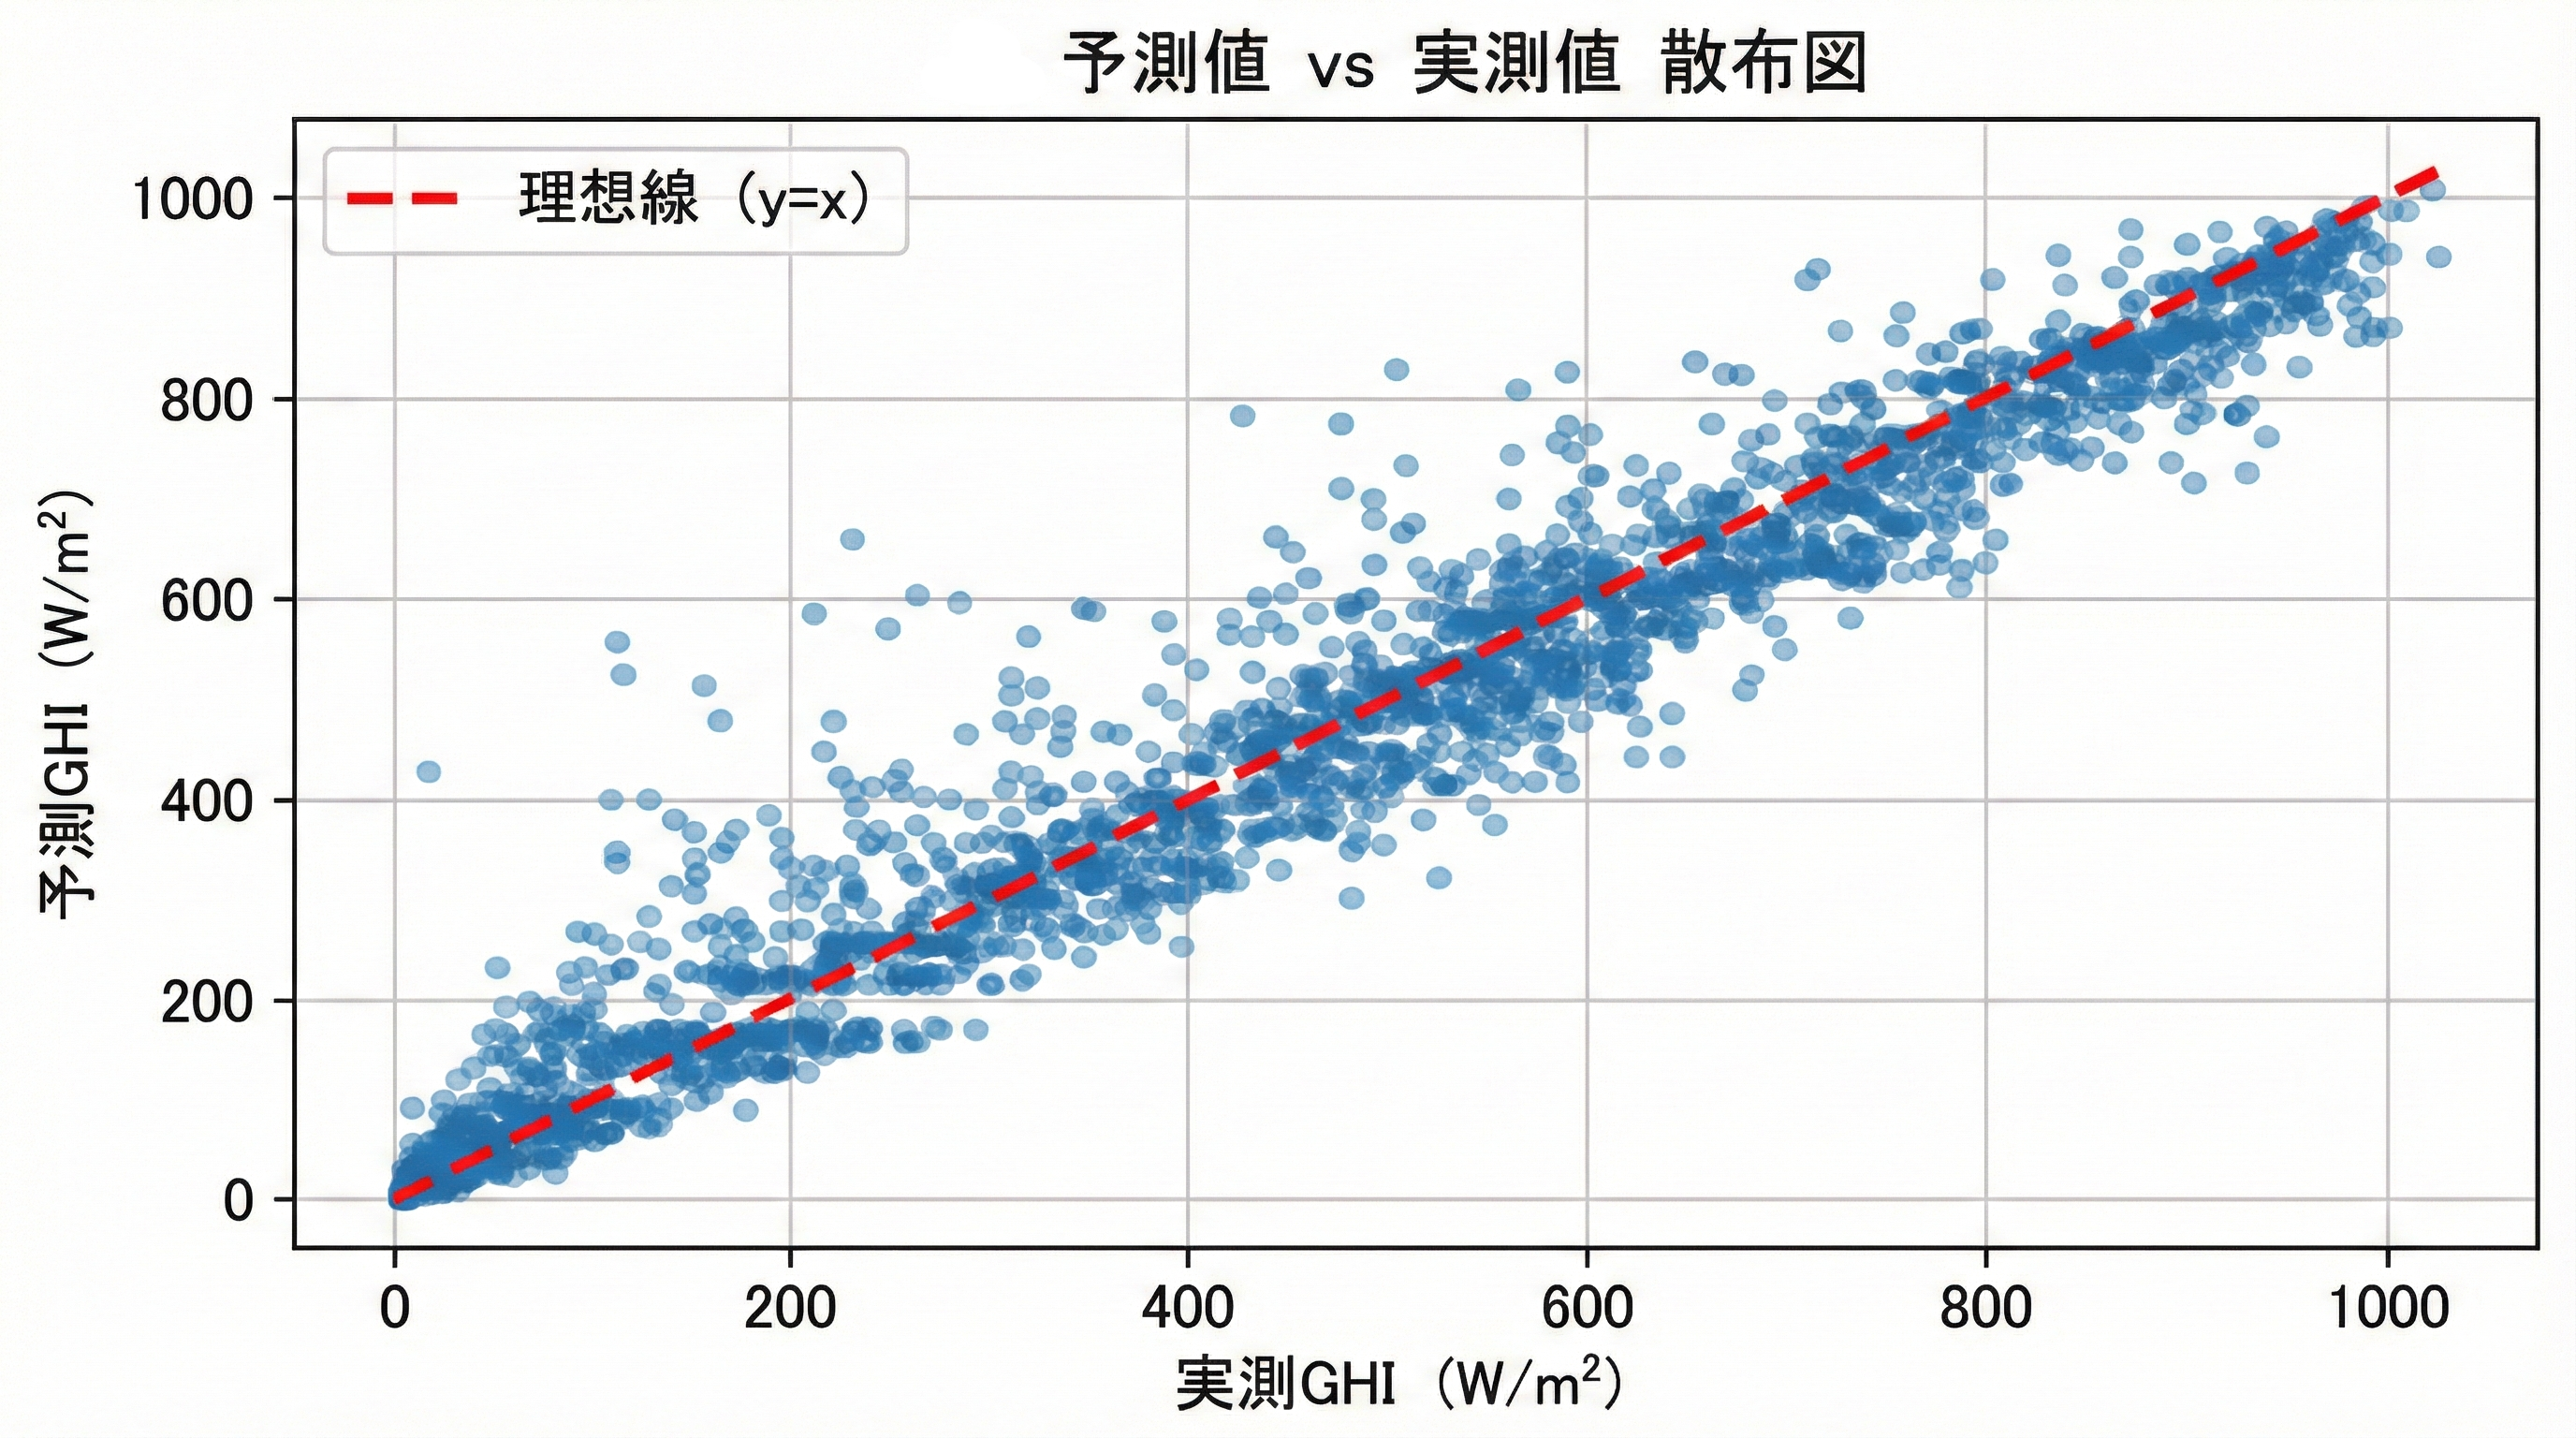
\includegraphics[width=0.9\textwidth]{foto/Hokuto/ScatterPlot.png}
    \caption{推定日射量と実測日射量の相関散布図 (2023年)}
    \label{fig:scatter_plot}
\end{figure}
\FloatBarrier

%------------------------------------------------------------------------
\subsection{誤差分布の統計的特性}
\label{subsec:誤差分布の統計的特性}
%------------------------------------------------------------------------

モデルの偏りを評価するため、推定誤差($Error = GHI_{est} - GHI_{meas}$)のヒストグラムを図\ref{fig:error_dist}に示す。

図中の緑色の破線で示される通り、全データの平均バイアス誤差(MBE)は \textbf{$-1.4 \mathrm{W/m^2}$} と極めて小さな値となった。これは、水平面日射量の最大値が 1000 $\mathrm{W/m^2}$ を超えることを考慮すると、実質的にバイアスフリーな推定が実現できていることを意味する。

また、分布形状はゼロを中心とした正規分布に近い形状を示しており、特定の条件下で一方向に誤差が偏る系統的な問題が排除され、残差がランダム成分主体となっていることが示唆される。

\begin{figure}[htbp]
    \centering
    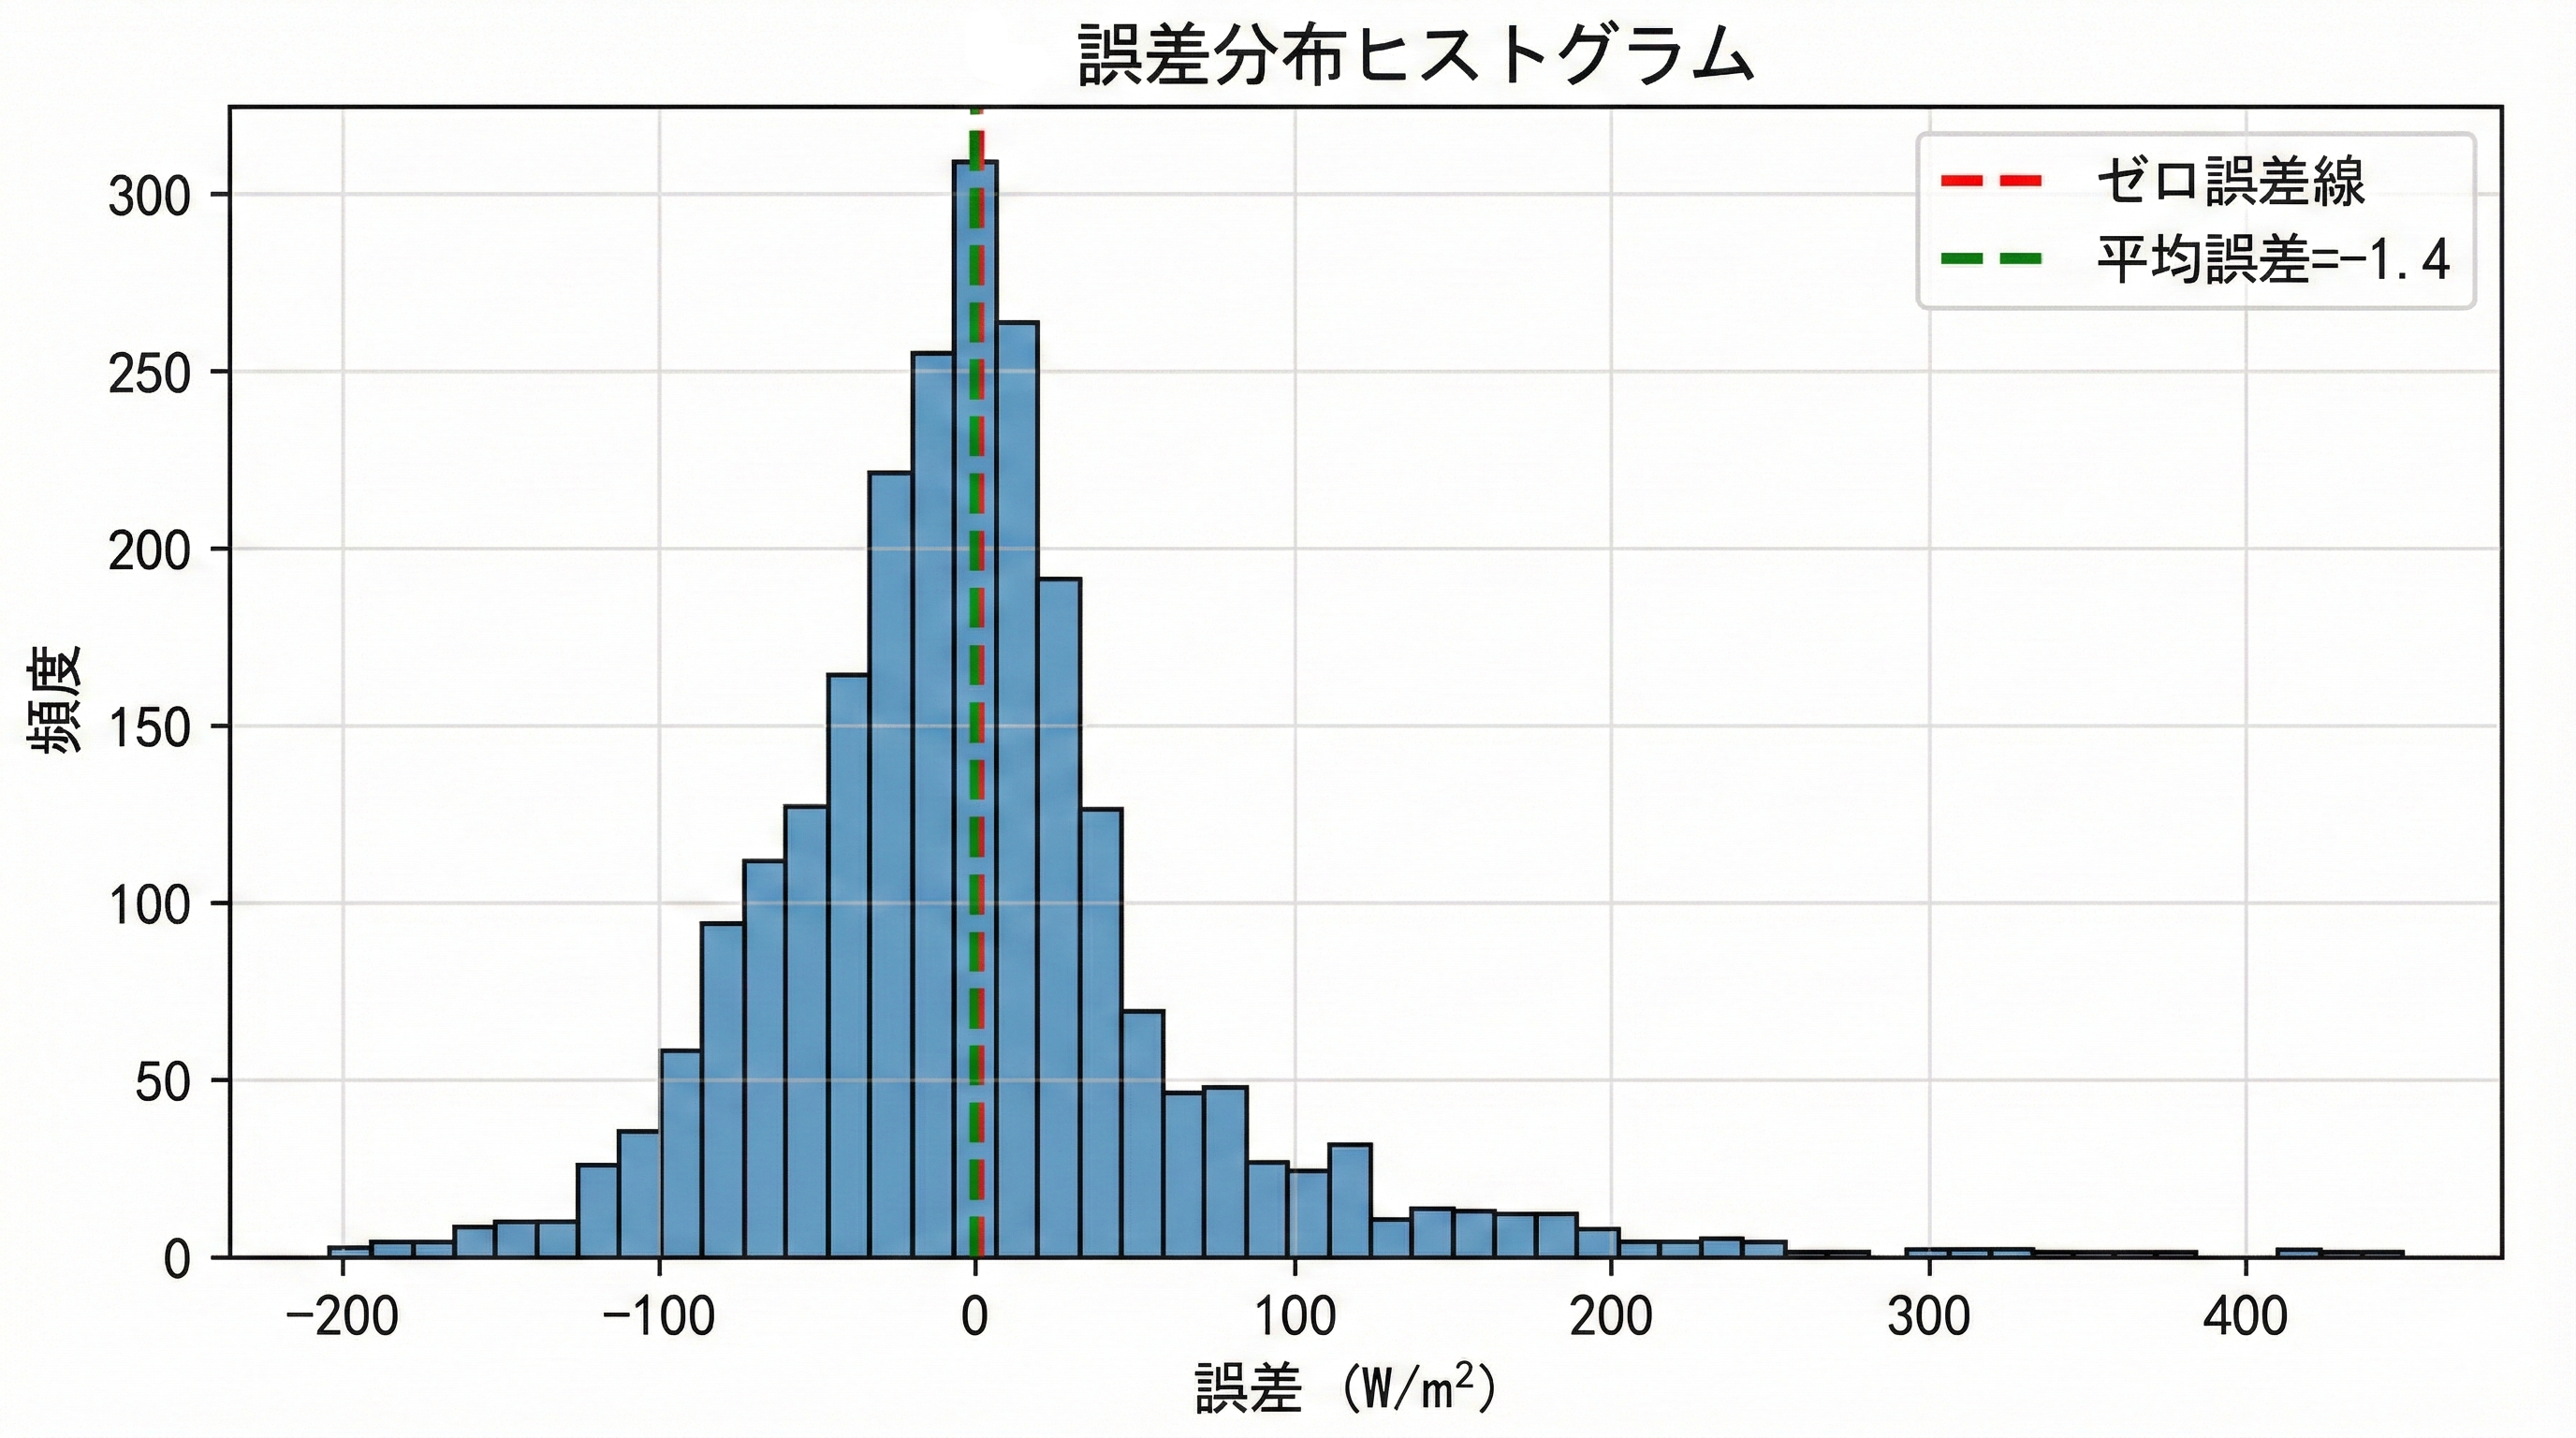
\includegraphics[width=0.9\textwidth]{foto/Hokuto/ErrorDistribution.png}
    \caption{推定誤差の頻度分布ヒストグラム(平均誤差 MBE = -1.4 $\mathrm{W/m^2}$)}
    \label{fig:error_dist}
\end{figure}
\FloatBarrier

%------------------------------------------------------------------------
\subsection{相対誤差による評価}
\label{subsec:相対誤差による評価}
%------------------------------------------------------------------------

図\ref{fig:rel_error_dist}に、相対誤差(Relative Error)の分布を示す。
ヒストグラムのピークは相対誤差 0.0(0\%)の地点に鋭く形成されており、大部分のデータが $\pm 20\%$ 以内の範囲に収まっている。一方で、相対誤差 $+1.0$(+100\%)付近に小さなピークが確認されるが、これは日出・日没直前などの実測値が極めてゼロに近い(数 $\mathrm{W/m^2}$)タイミングにおいて、わずかな推定値(例:10 $\mathrm{W/m^2}$)が存在することで計算上大きな比率となったものであり、エネルギー総量としての影響は軽微である。

\begin{figure}[htbp]
    \centering
    \includegraphics[width=0.9\textwidth]{foto/Hokuto/RelativeErrorDistribution.png}
    \caption{相対誤差の頻度分布}
    \label{fig:rel_error_dist}
\end{figure}
\FloatBarrier

以上の結果より、提案手法は水平面日射量の大小にかかわらず、通年で安定して高い推定精度を有していると結論付けられる。

%------------------------------------------------------------------------
\subsection{残差分布のトレンド分析}
\label{subsec:残差分布のトレンド分析}
%------------------------------------------------------------------------

前節では全体平均としてのバイアスが除去されていることを確認したが、水平面日射量のレンジごとの微視的な挙動を確認するため、実測 GHI に対する残差の分布特性を解析する。

図\ref{fig:error_bias_scatter}に、横軸を実測 GHI、縦軸を推定誤差とした残差プロットを示す。

全体として、誤差はゼロライン(赤破線)を中心に分布しているものの、水平面日射量の変化に伴って分布の中心が緩やかに変動する「逆S字型」に近いトレンドが確認された。具体的には、低~中照度域では過大評価に、高照度域では過小評価にデータが偏る傾向が見られる。

\begin{figure}[htbp]
    \centering
    \includegraphics[width=0.8\textwidth]{foto/Hokuto/ErrorBiosDetect.png}
    \caption{実測GHIに対する残差分布}
    \label{fig:error_bias_scatter}
\end{figure}
\FloatBarrier

%------------------------------------------------------------------------
\subsection{強度区分ごとの定量的評価と物理的考察}
\label{subsec:強度区分ごとの定量的評価と物理的考察}
%------------------------------------------------------------------------

この傾向を定量化するため、GHI を $100 \mathrm{W/m^2}$ 刻みで区分し、各区間の平均誤差を算出した結果を図\ref{fig:avg_error_ghi}に示す。この結果に基づき、各領域の物理的挙動を以下のように考察する。

\begin{figure}[htbp]
    \centering
    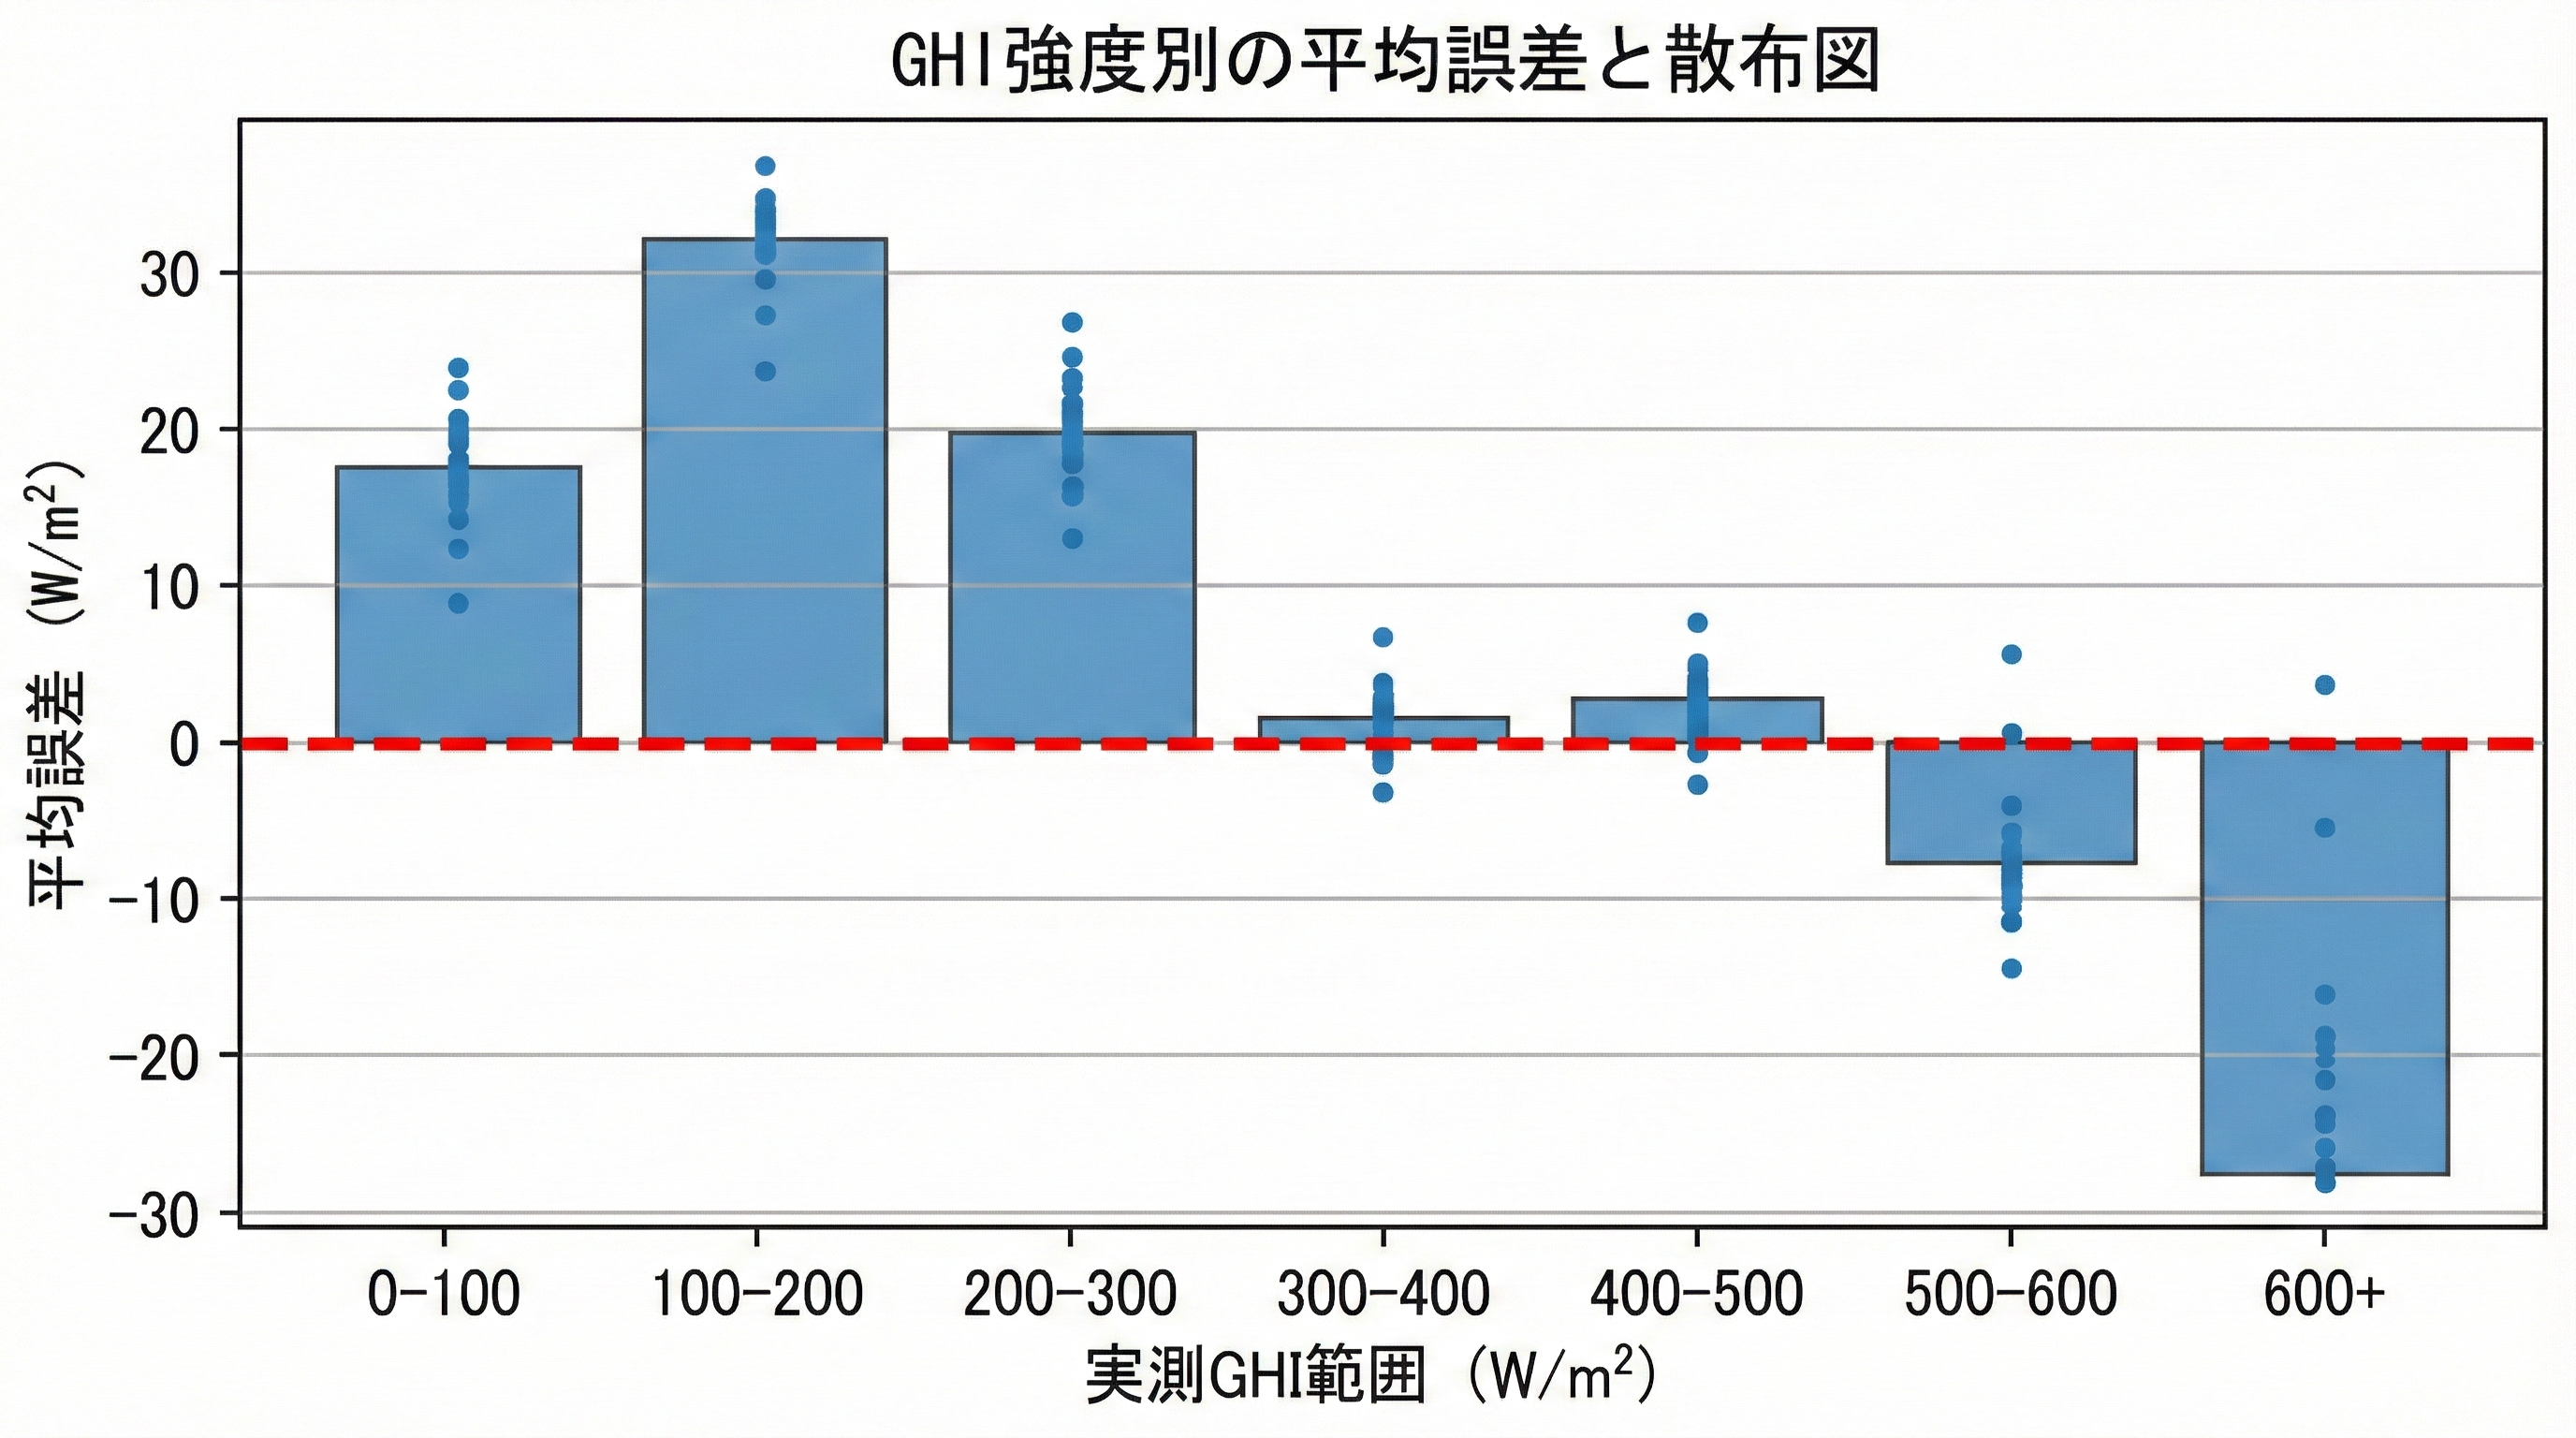
\includegraphics[width=0.8\textwidth]{foto/Hokuto/AverageErrorInDifferentGHI.png}
    \caption{GHI強度別の平均誤差と散布図}
    \label{fig:avg_error_ghi}
\end{figure}

\begin{enumerate}
    \item \textbf{中照度域($100 \sim 300$ $\mathrm{W/m^2}$)における正のバイアス}: \\
    図\ref{fig:avg_error_ghi}によると、特に $100 \sim 200 \mathrm{W/m^2}$ の区間において、平均 $+30 \mathrm{W/m^2}$ 前後の最も顕著な過大推定が確認された。
    この領域は、厚い雲に覆われた散乱日射主体の条件、あるいは雲の切れ間から強い反射光が入射する条件に相当する。散乱成分が多い環境下では、PVモジュールが特定の角度からの散乱光を効率よく受光し、理論モデル(直達成分主体で計算される $PoA$)が想定するよりも高い出力を生成する場合がある。これにより、逆推定モデルは実際の全天日射量よりも高い値を算出してしまったと考えられる。

    \item \textbf{中間遷移域($300 \sim 500$ $\mathrm{W/m^2}$)の安定性}: \\
    $300 \sim 500 \mathrm{W/m^2}$ の範囲では、平均誤差がほぼ $0 \mathrm{W/m^2}$ に収束しており、物理モデルとシステム挙動が最も良く整合している。この領域は、部分的な晴天時においてシステムがリニアな特性を維持しやすい「スイートスポット」であると言える。

    \item \textbf{高照度域(600 $\mathrm{W/m^2}$ 以上)における負のバイアス}: \\
    $600 \mathrm{W/m^2}$ を超える高照度域では、水平面日射量の増加に伴い負のバイアス(過小推定)が拡大し、最大で $-28 \mathrm{W/m^2}$ 程度の過小評価となっている。
    この要因としては、以下の2点が推察される。
    \begin{itemize}
        \item \textbf{温度補正の残留誤差}: 高日射時はモジュール温度が著しく上昇するため、物理モデルの温度係数 $\gamma$ による補正が追いつかず、熱損失による出力低下を「日射不足」と誤認している可能性。
        \item \textbf{PCSの変換限界}: 定格出力付近でのPCSの変換効率低下や、微細な出力抑制挙動により、入力される日射エネルギーに対して出力電力 $P_{DC}$ の伸びが鈍化し、結果として低い日射量が逆算された可能性が高い。
    \end{itemize}
\end{enumerate}

以上の分析より、提案モデルは全体として高精度であるものの、極端な気象条件下(散乱光主体または高熱負荷時)においては、物理的な制約に起因するわずかな非線形バイアスが残留していることが明らかとなった。

%------------------------------------------------------------------------
\subsection{時刻別の誤差分散特性}
\label{subsec:時刻別の誤差分散特性}
%------------------------------------------------------------------------

続いて、推定誤差の時間帯による変動(周特性)および季節による偏りについて詳細な分析を行う。

図\ref{fig:hourly_error}に、時刻ごとの誤差分布を示すボックスプロットを示す。

正午付近(11:00 ~ 13:00)において、箱ひげ図の四分位範囲および外れ値の範囲が最大となっている。一見すると精度が悪化しているように見えるが、これは当該時間帯の水平面日射量の絶対量が大きいため、相対的な誤差率としては許容範囲内である。実際、中央値(オレンジ色の線)は全時間帯を通じてゼロライン付近を推移しており、モデルが日中のピーク電力を正しく捉えていることが分かる。

一方で、15:00 ~ 16:00 の時間帯において、分布全体が負の方向へシフトする傾向が見られる。これは、西日による建物の影や、夕方の急激な気温低下に伴うパネル温度特性の変化が影響していると推察される。

\begin{figure}[htbp]
    \centering
    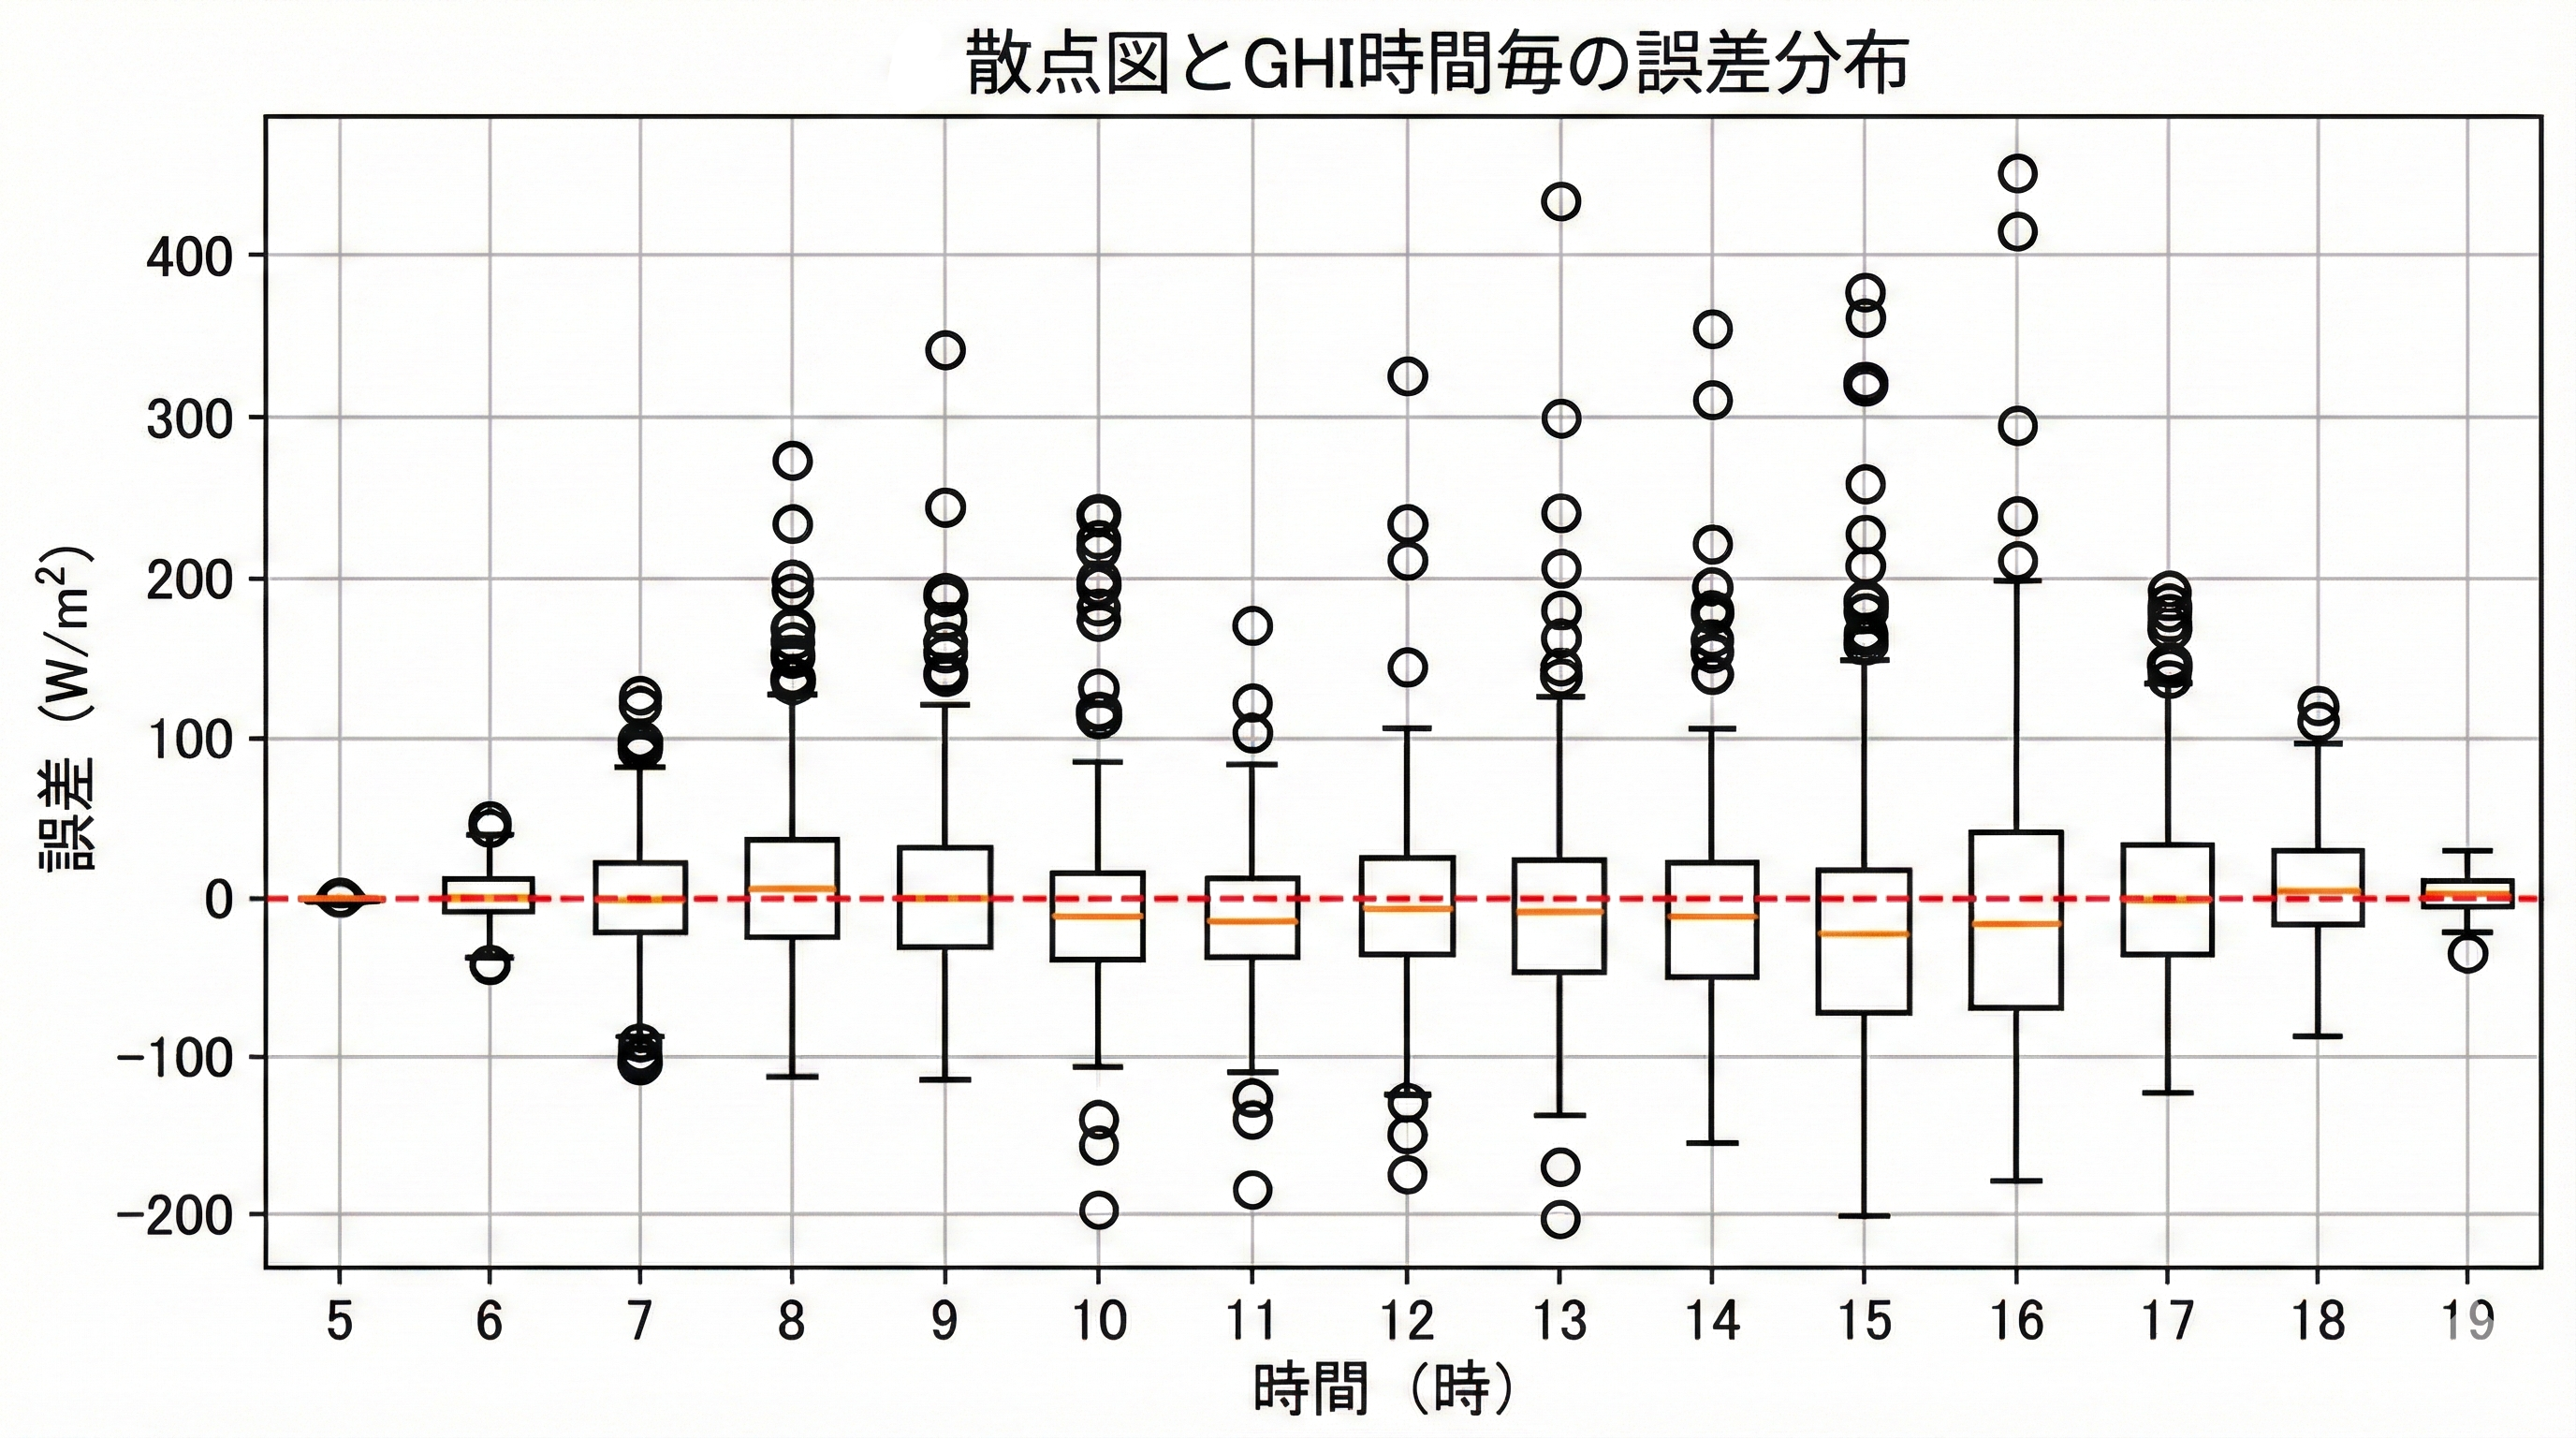
\includegraphics[width=0.8\textwidth]{foto/Hokuto/GHIErrorDistributionPerHour.png}
    \caption{時刻別GHI推定誤差の分布}
    \label{fig:hourly_error}
\end{figure}
\FloatBarrier

%------------------------------------------------------------------------
\subsection{月別平均誤差と季節特有のバイアス}
\label{subsec:月別平均誤差と季節特有のバイアス}
%------------------------------------------------------------------------

図\ref{fig:monthly_error}に、月ごとの平均誤差を示す。

多くの月で誤差は $\pm 10 \mathrm{W/m^2}$ 以内に収まっているが、9月および10月において、それぞれ $-22 \mathrm{W/m^2}$、$-32 \mathrm{W/m^2}$ という顕著な過小評価が確認された。

この要因としては、以下の2点が考えられる。

\begin{enumerate}
    \item \textbf{秋季特有の気象条件}: 秋雨前線や台風の影響により、雲の移動速度が速く日射変動が激しい日が多いため、1時間平均処理の過程で瞬時値ベースの物理モデルとの乖離が生じやすい。
    \item \textbf{太陽高度低下による影の影響}: 夏至を過ぎて太陽高度が低下し始める時期であり、特定の障害物による影がパネルにかかり始める初期段階である可能性が高い。この「影による出力低下」を、モデルが「日射不足」と判断して推定値を下げていることが、負のバイアスの主因と考えられる。この点については、第\ref{subsec:日陰検出結果と重要度分析}節の日陰検出結果にて詳細に検証する。
\end{enumerate}

\begin{figure}[htbp]
    \centering
    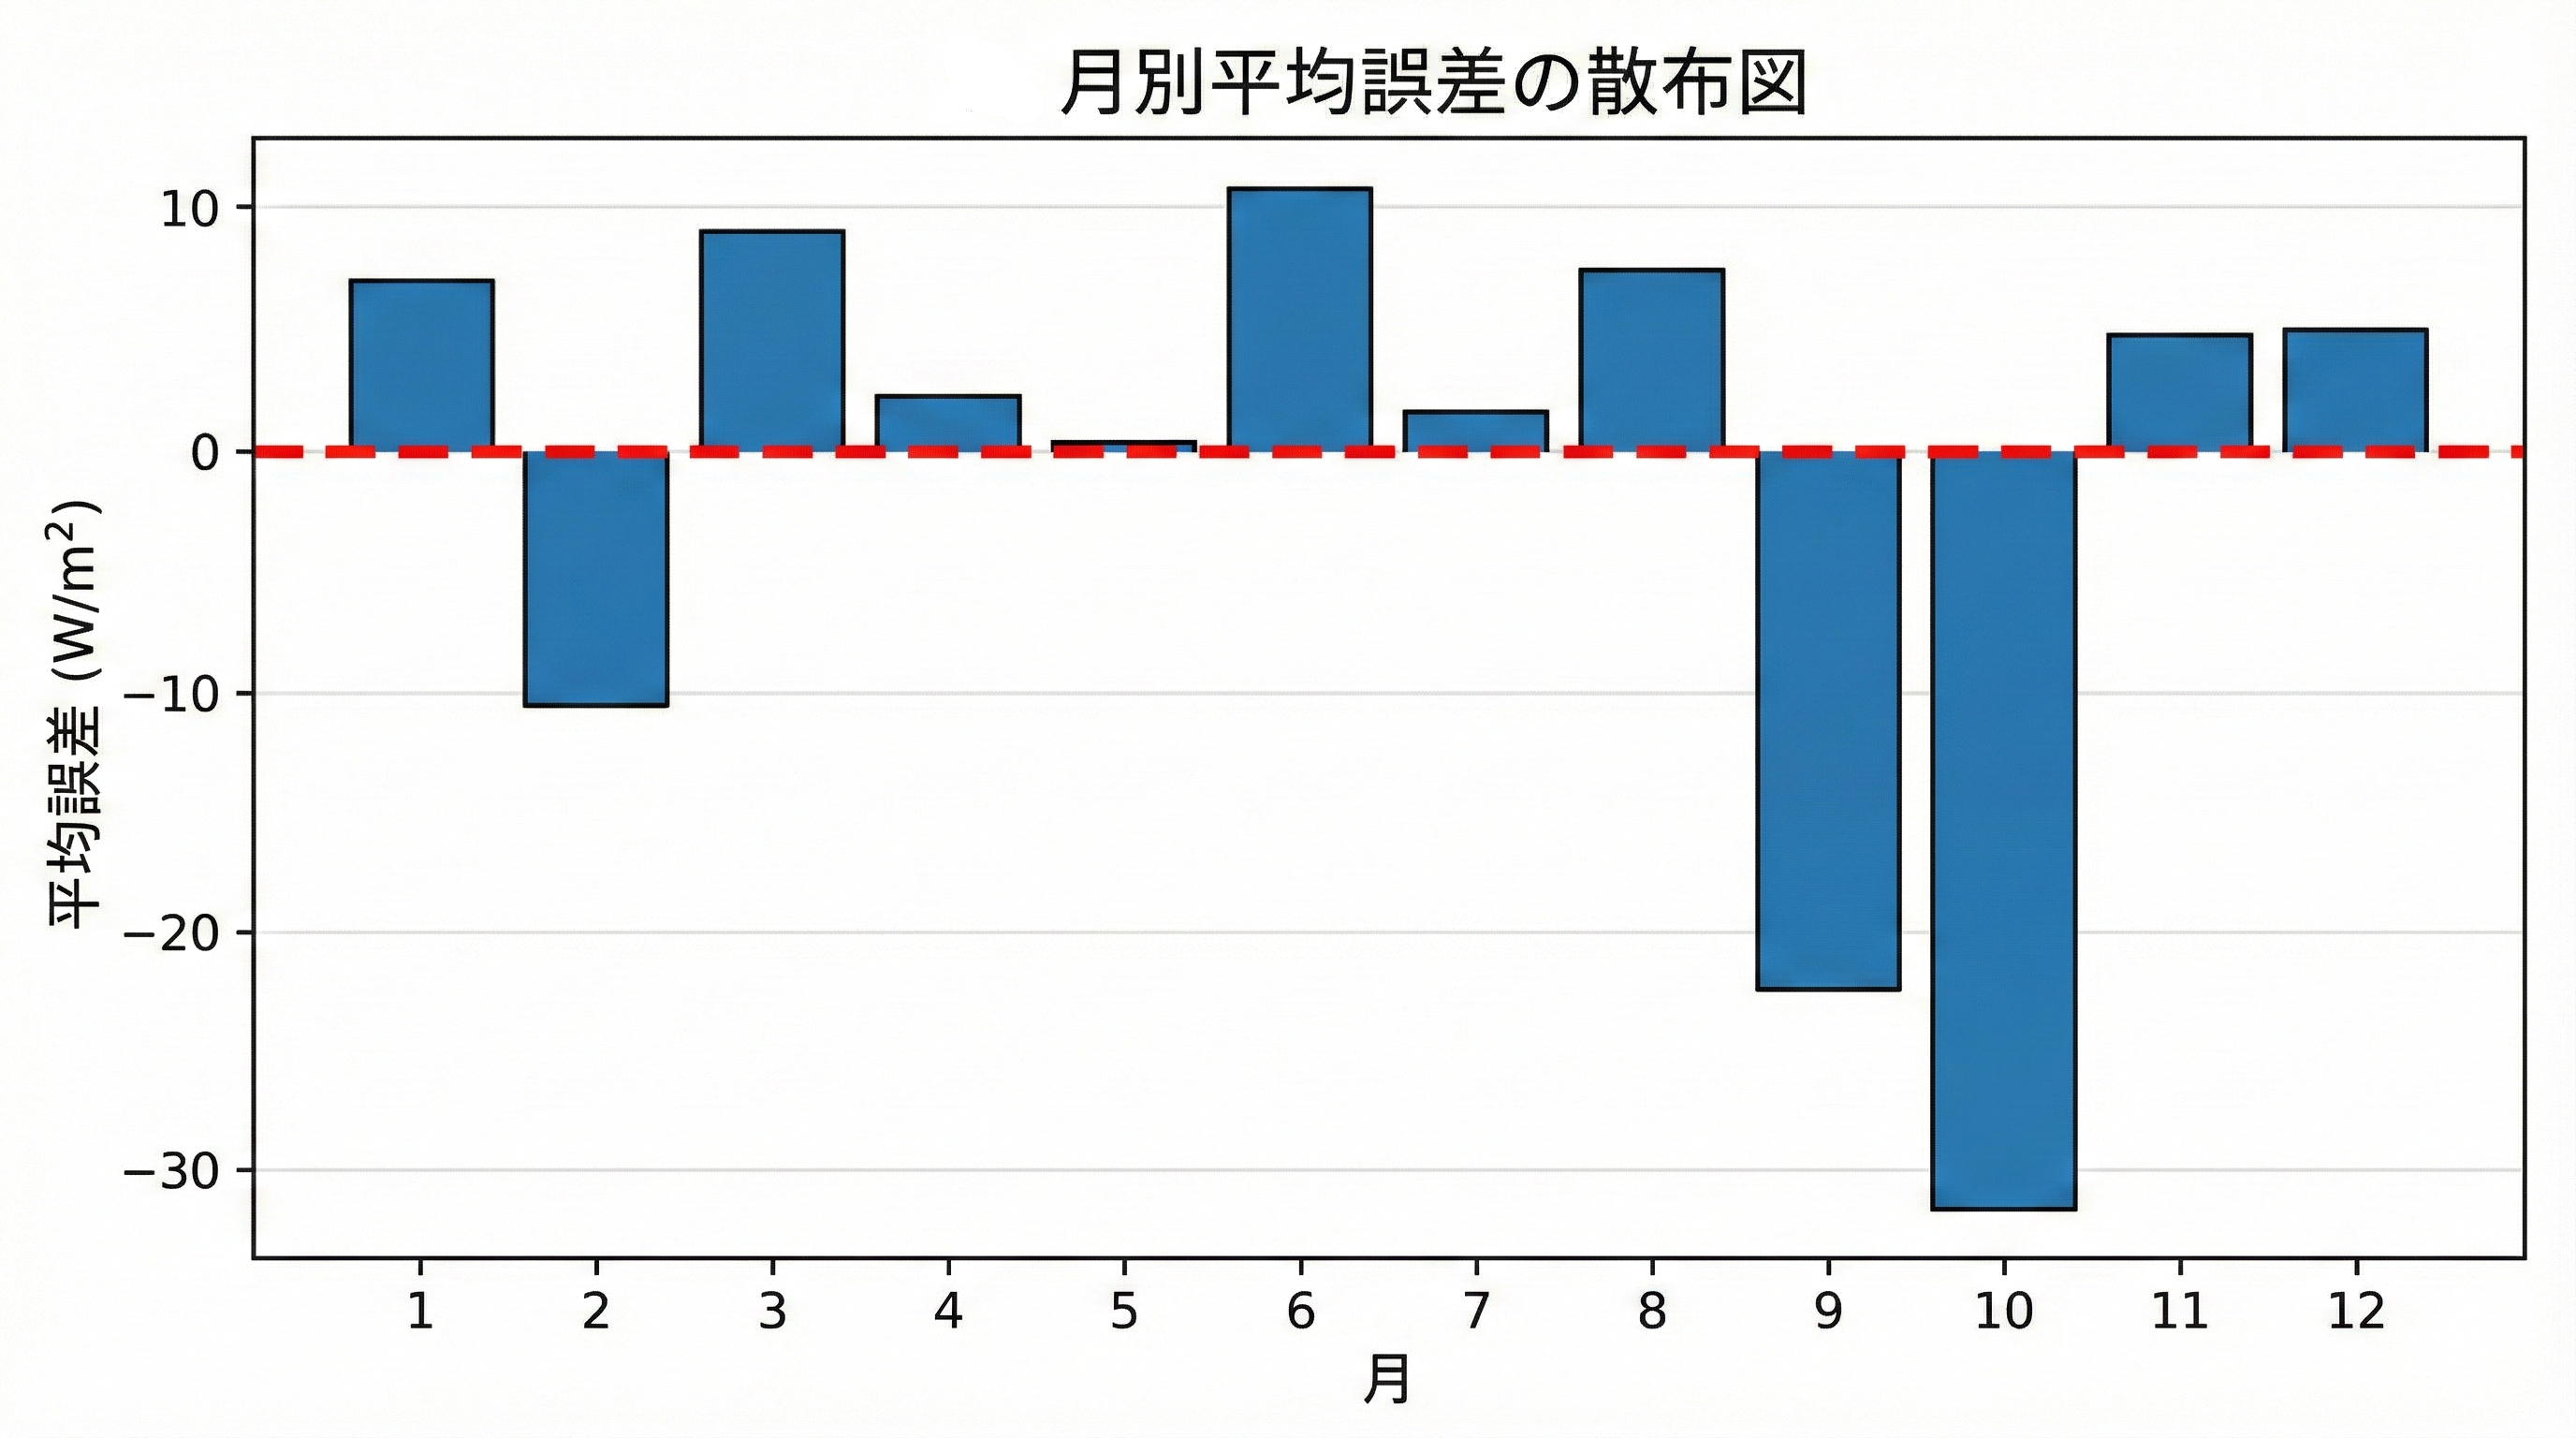
\includegraphics[width=0.9\textwidth]{foto/Hokuto/MonthErrorDistributionScatterPlot.png}
    \caption{月別平均誤差の推移}
    \label{fig:monthly_error}
\end{figure}
\FloatBarrier

%------------------------------------------------------------------------
\subsection{長期的トレンドと経年劣化補正の妥当性}
\label{subsec:長期的トレンドと経年劣化補正の妥当性}
%------------------------------------------------------------------------

図\ref{fig:weekly_trend}に、2023年の第1週から第52週までの週間平均誤差の時系列推移を示す。

緑色の破線で示される線形トレンドラインの傾きは$-0.090$であり、年間を通じて誤差のベースラインがほぼ水平(フラット)に保たれていることが確認できる。

第\ref{sec:月間平均トレンドによる影の影響評価}節においてシステム劣化率($-1.31\%$/年)に基づく $K_0$ の事前補正を行わなかった場合、このトレンドラインは右肩下がりの負の傾きを示すはずである。したがって、傾きがほぼゼロであるという結果は、提案した経年劣化補正アルゴリズムが適切に機能し、長期的なドリフト誤差を抑制できていることの強力な証左である。

\begin{figure}[htbp]
    \centering
    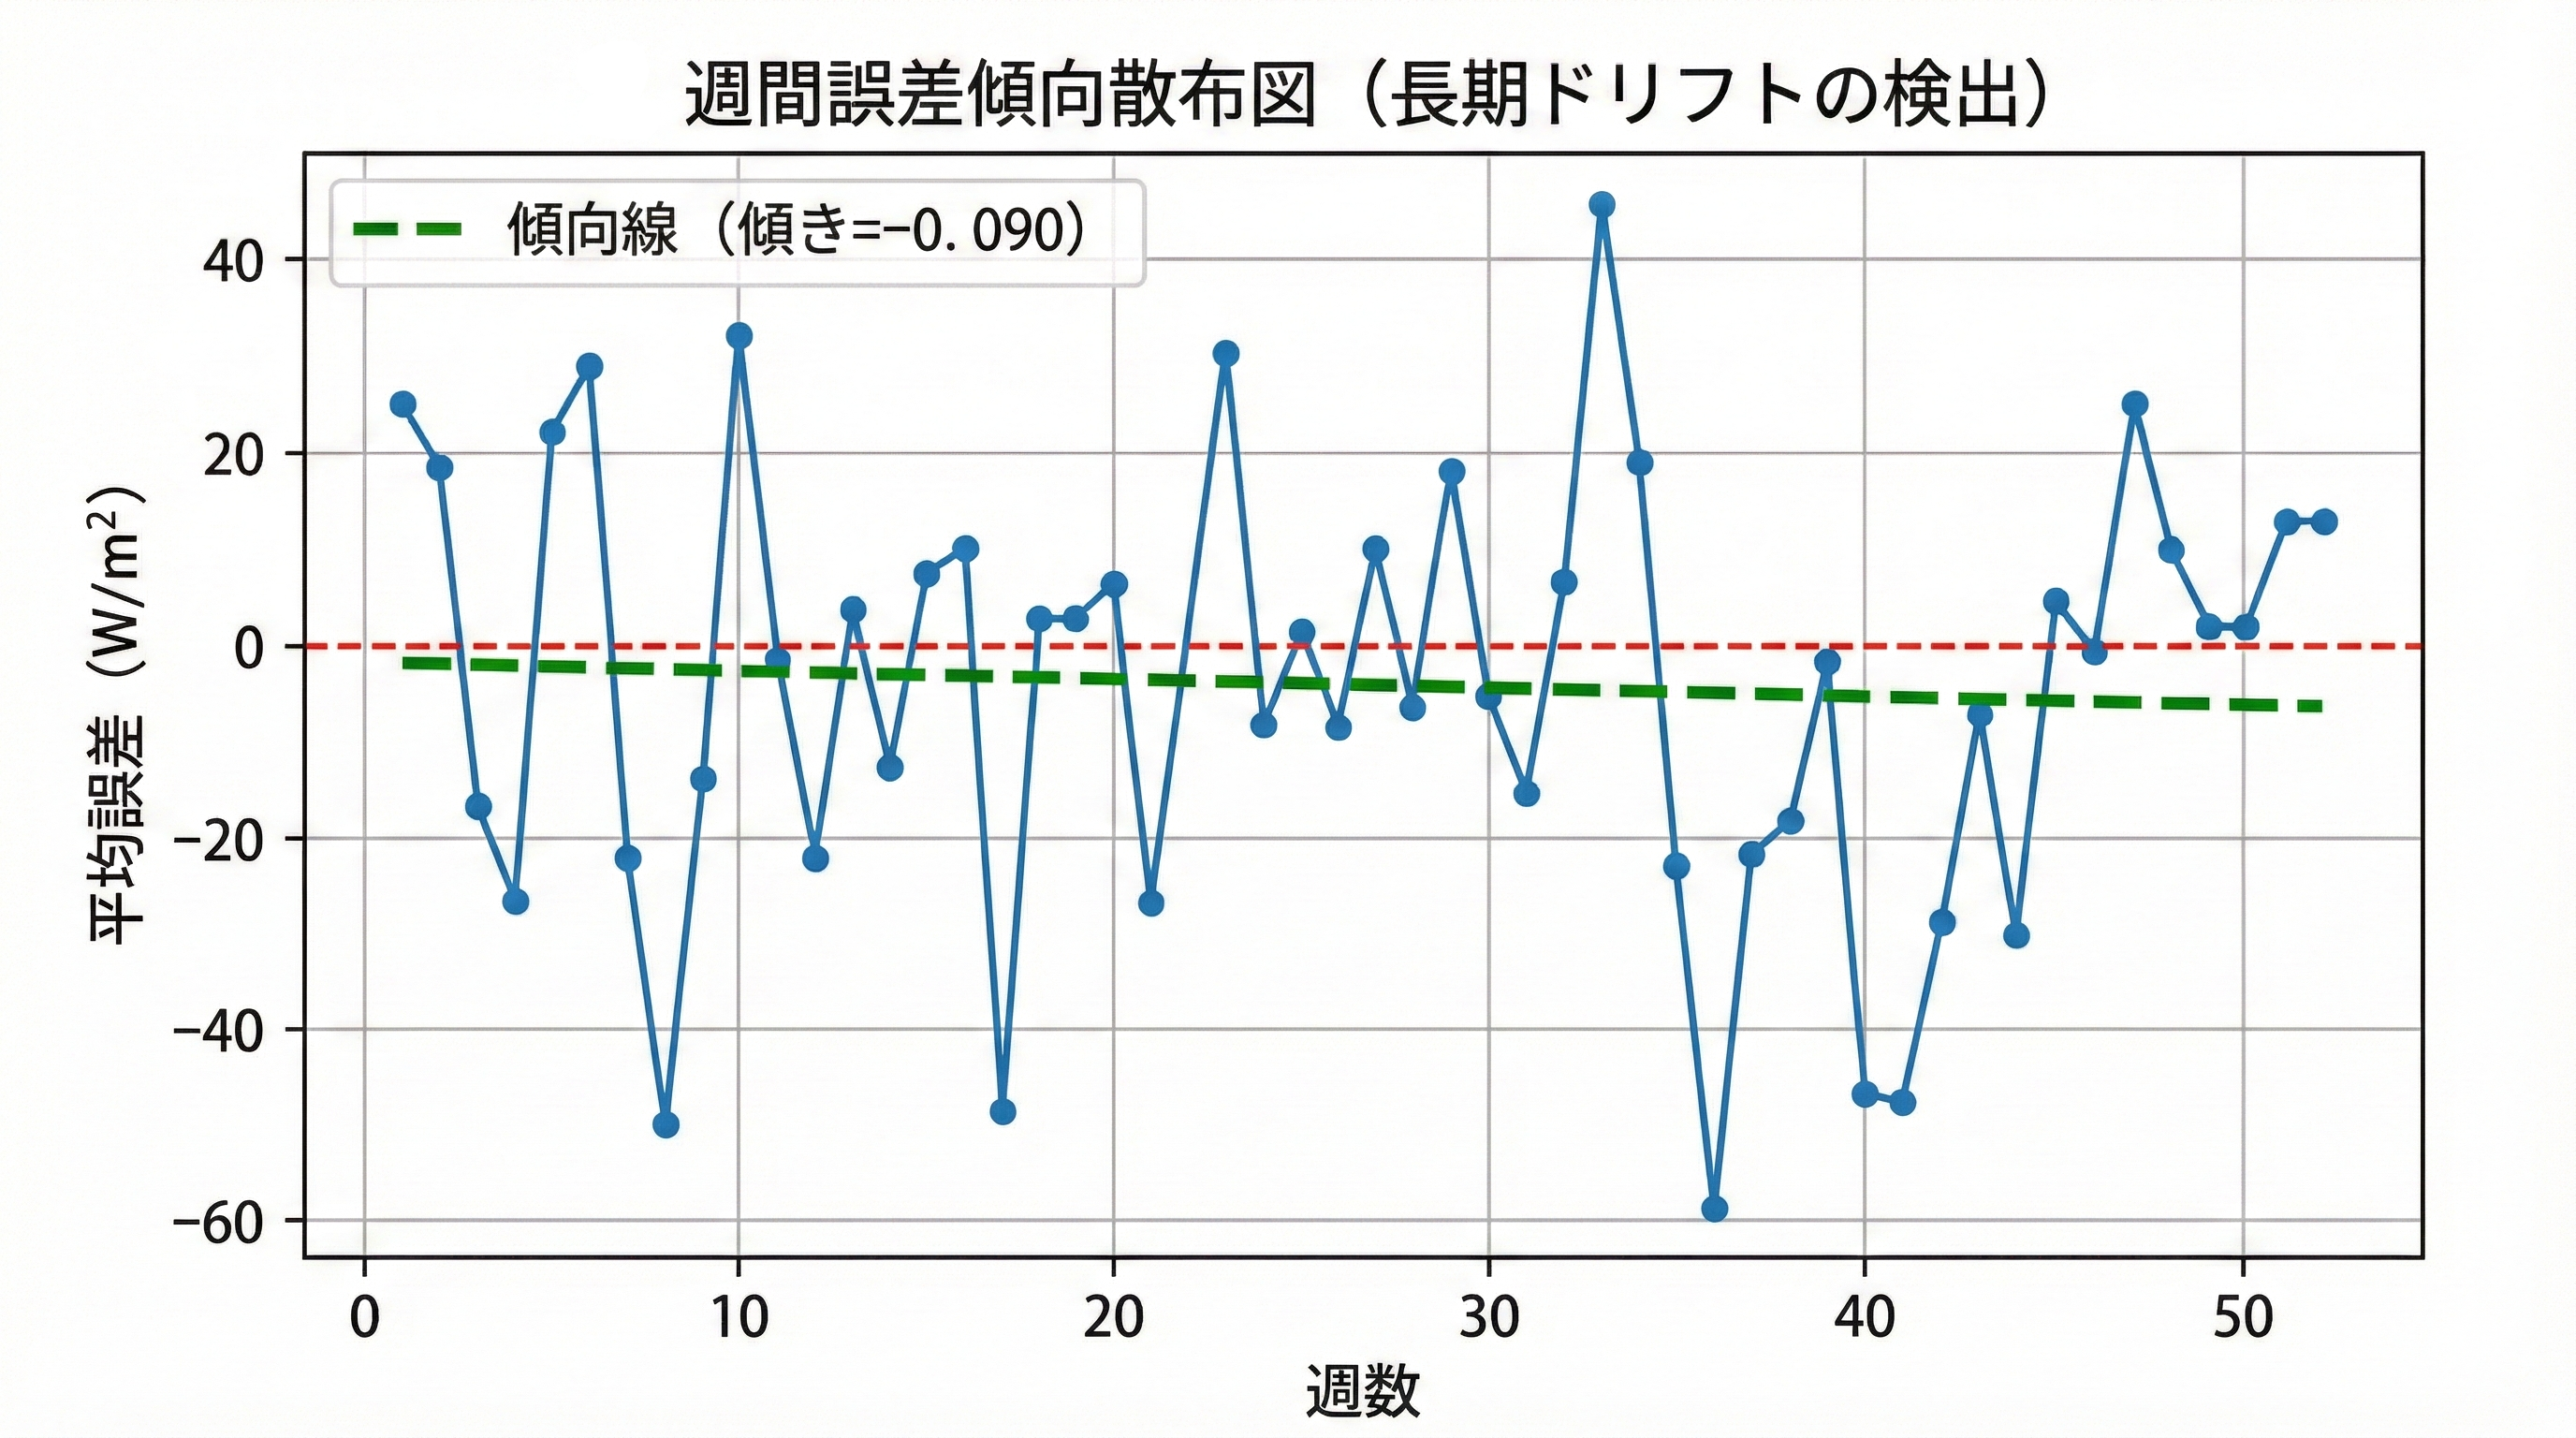
\includegraphics[width=0.8\textwidth]{foto/Hokuto/ErrorTrendInDifferentWeek.png}
    \caption{週間平均誤差の時系列トレンド(傾き -0.090)}
    \label{fig:weekly_trend}
\end{figure}
\FloatBarrier

%------------------------------------------------------------------------
\subsection{モデル別誤差分布の比較}
\label{subsec:モデル別誤差分布の比較}
%------------------------------------------------------------------------

図\ref{fig:ml_vs_ko}に、MLモデルによって推定されたデータ群(青色)と、物理モデルによって推定されたデータ群(橙色)の誤差分布ヒストグラムを重ねて示す。

\begin{figure}[htbp]
    \centering
    \includegraphics[width=0.8\textwidth]{foto/Hokuto/ErrorDistributionBetweenMLandKo.png}
    \caption{機械学習モデル(ML)と物理モデル($K_0$)の誤差分布比較}
    \label{fig:ml_vs_ko}
\end{figure}
\FloatBarrier

この図から、両モデルの特性には以下の明確な差異が確認できる。

\begin{enumerate}
    \item \textbf{MLモデルの高精度な収束(青色)}:
    MLモデルの分布は、ゼロ誤差ライン(赤破線)付近に極めて鋭いピーク(高い尖度)を形成しており、分布の裾野(外れ値)が非常に狭いことが分かる。
    通常、低照度域はPCSの起動電圧特性や内部損失の影響を受けやすく、物理モデル単体では誤差が発散しやすい「難所」である。しかし、図示された結果は、電圧情報を用いたMLモデルがこの非線形性を的確に学習し、物理モデル以上の精度で日射量を逆推定できていることを証明している。

    \item \textbf{物理モデルの分散特性(橙色)}:
    一方、物理モデル($K_0$)の分布は、正規分布に近い形状をしているものの、MLモデルと比較して分散の横幅が大きい。これは、物理モデルが担当する中・高照度域においては、日射エネルギーの絶対量が大きく、かつ温度やスペクトル変化といった物理的変動要因の影響を強く受けるためである。
\end{enumerate}

%************************************************************************
\section{K-means法による相互比較}
\label{subsec:K-means法による相互比較}
%************************************************************************

本項では、前節で構築したK-means法に基づく残差クラスタリングを、正常稼働システム(Sys21)および日陰の影響が疑われるシステム(Sys17)の双方に適用し、その統計的差異を明らかにする。

図\ref{fig:cluster_average_comparison}に、Sys21およびSys17において分類された各クラスタ($k=3$)の平均残差(Average Residual)を示す。

正常なシステムであるSys21(図\ref{fig:cluster_average_comparison}(a))においては、主要なクラスタ(Cluster 2, 3)の平均誤差がいずれも $0 \mathrm{kW}$ 付近に収束している。Cluster 1 において負の大きな値が見られるが、これは積雪や通信エラー等の突発的な外れ値(Outliers)が分離されたものであり、データ全体に占める割合は低い。

対照的に、異常システムであるSys17(図\ref{fig:cluster_average_comparison}(b))では、Cluster 3 が **$-4.7 \mathrm{kW}$** という極めて大きな負の平均値を示している。これはシステムの定格容量(約10kW)の半数近くに達する損失であり、単なる気象ノイズでは説明がつかない、構造的かつ継続的な出力低下要因の存在を示唆している。

\begin{figure}[htbp]
    \centering
    \begin{minipage}[b]{0.48\textwidth}
        \centering
        \includegraphics[width=\textwidth]{foto/Hokuto/Sys21EachClusteringAverageError.png}
        \caption*{(a) Sys21(正常系)}
    \end{minipage}
    \hfill
    \begin{minipage}[b]{0.48\textwidth}
        \centering
        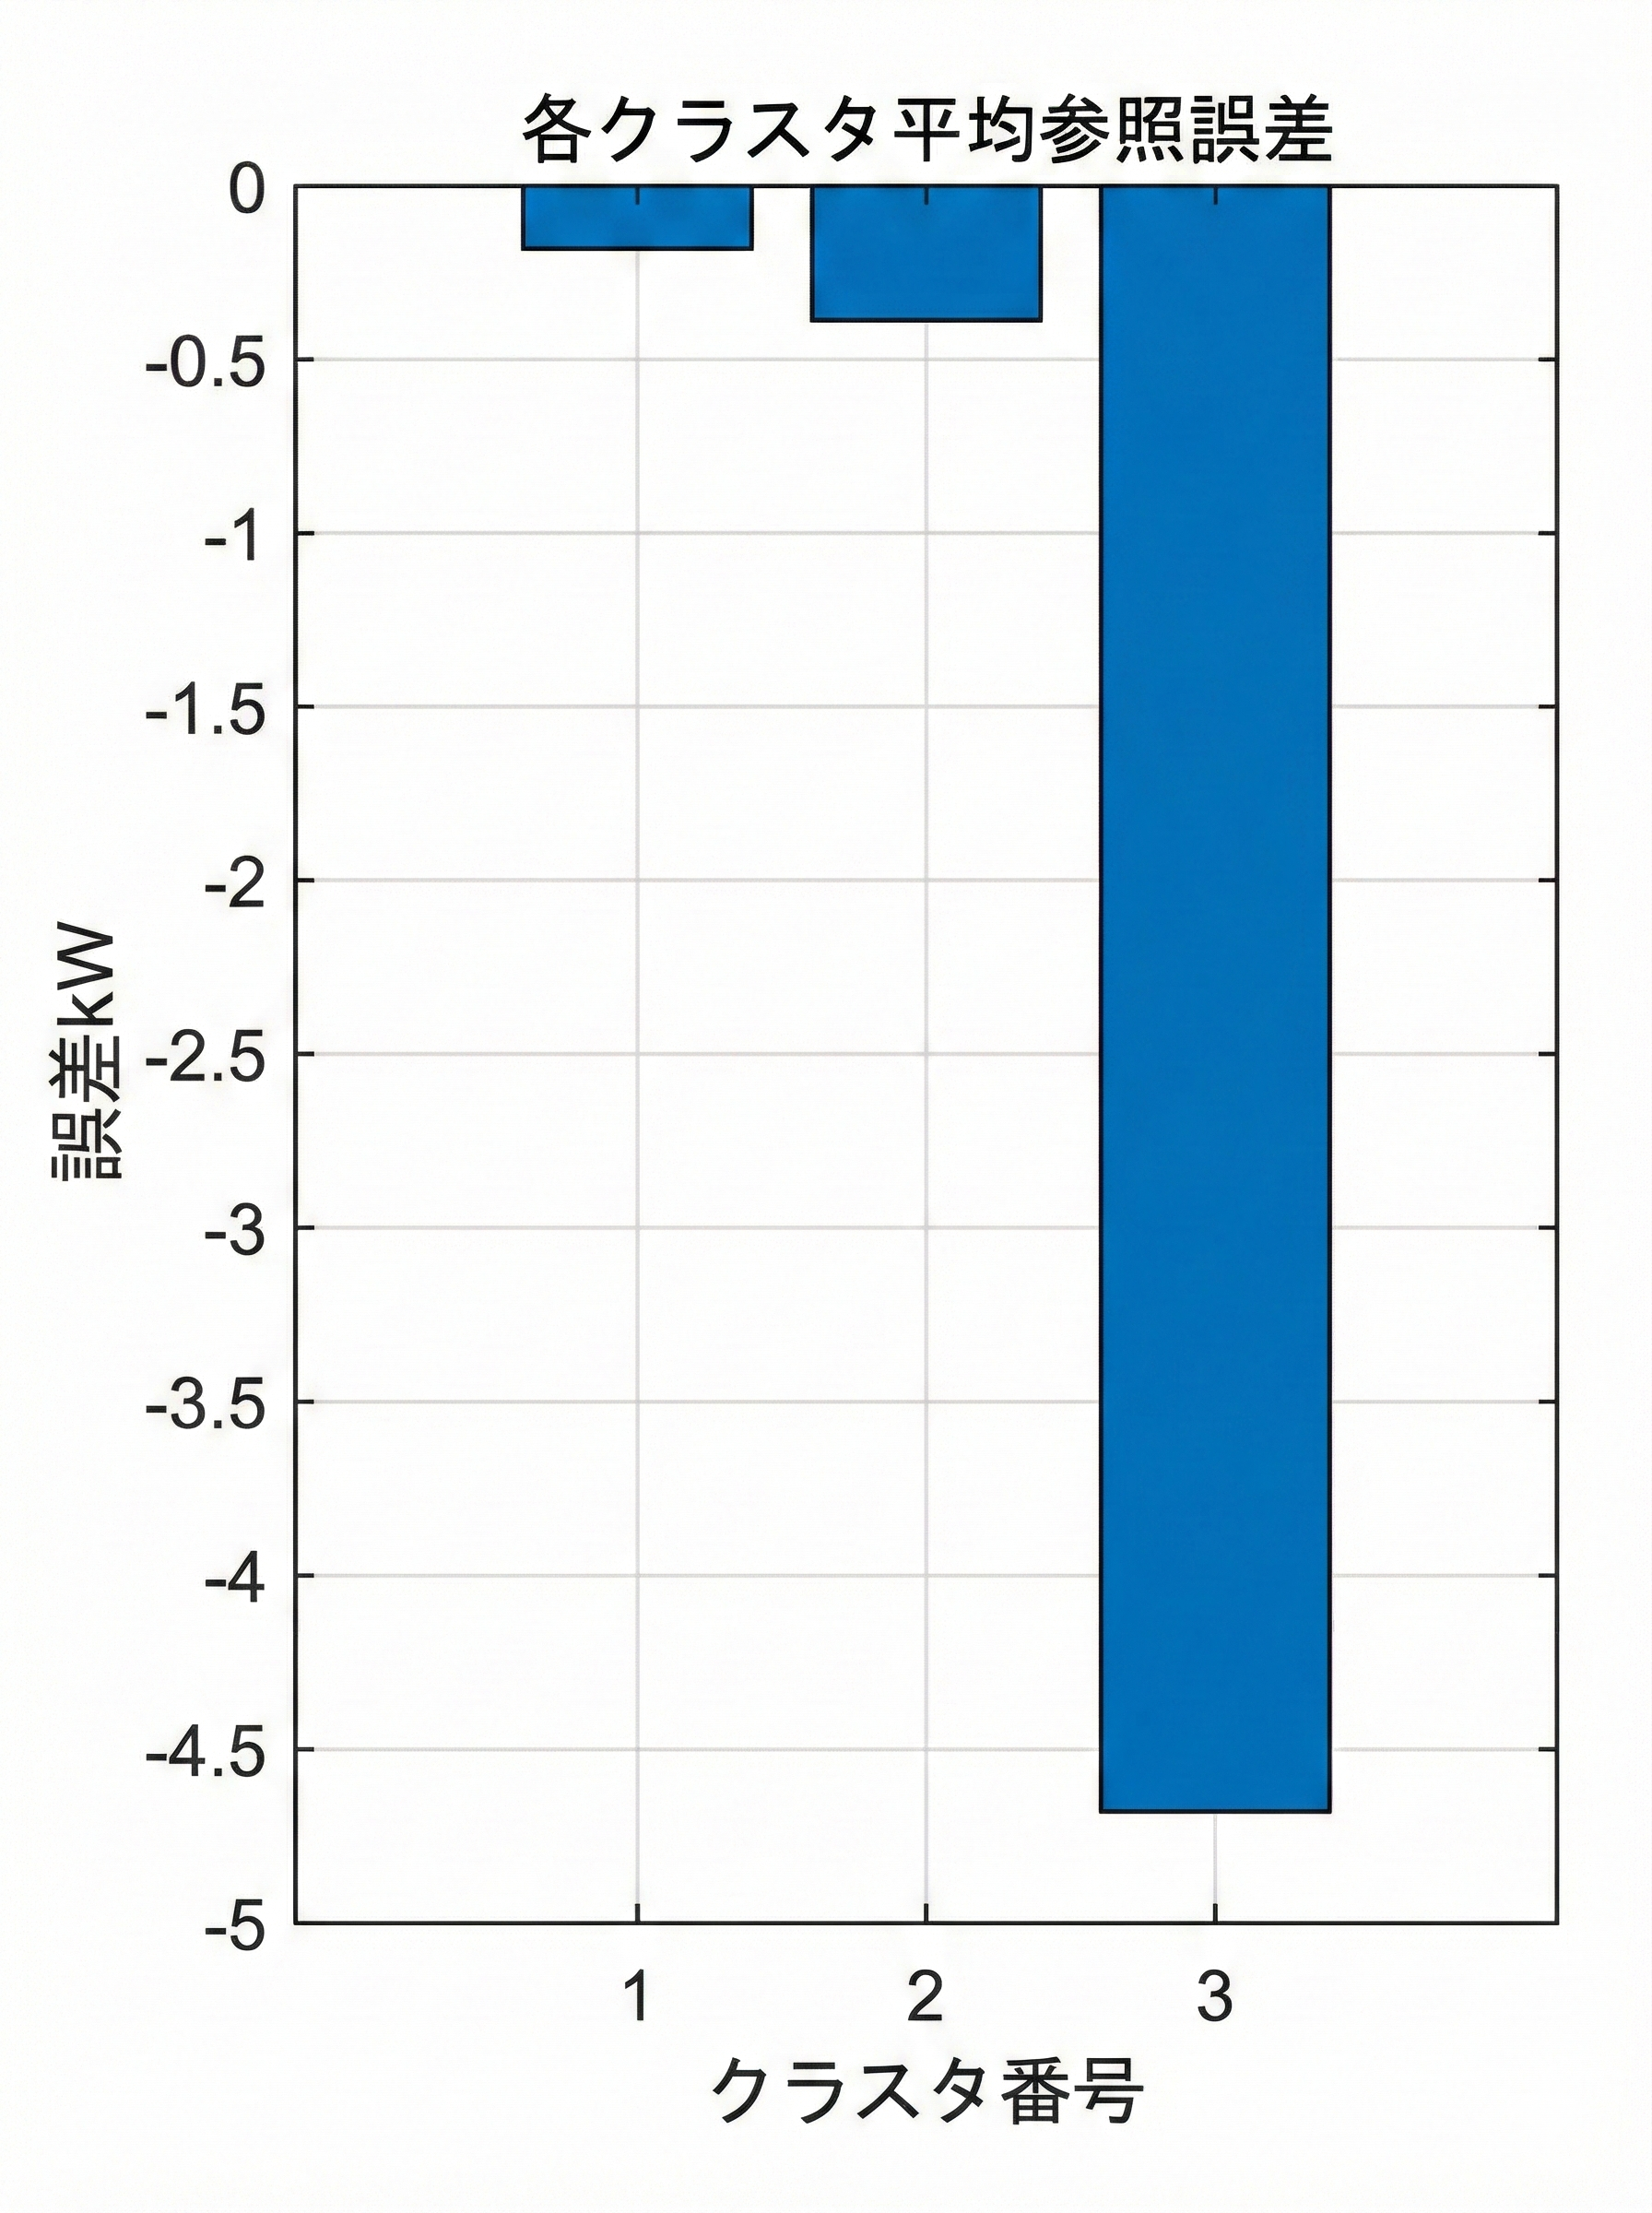
\includegraphics[width=\textwidth]{foto/Hokuto/Sys17EachClusteringAverageError.png}
        \caption*{(b) Sys17(異常系)}
    \end{minipage}
    \caption{K-means法により分類された各クラスタの平均誤差比較}
    \label{fig:cluster_average_comparison}
\end{figure}
\FloatBarrier

%------------------------------------------------------------------------
\subsection{太陽高度角に対する残差分布の構造解析}
\label{subsec:太陽高度角に対する残差分布の構造解析}
%------------------------------------------------------------------------

上記の統計的差異がどのような物理的条件下で発生しているかを確認するため、横軸に太陽高度角(Solar Altitude)、縦軸に推定誤差をとった散布図を図\ref{fig:cluster_scatter_comparison}に示す。図中の色は、K-means法によって割り当てられたクラスタラベル(黄色、青色、紫色)に対応している。

\begin{enumerate}
    \item \textbf{正常システム(Sys21)の挙動}: \\
    図\ref{fig:cluster_scatter_comparison}(a)に示す通り、Sys21のデータ点(特に主要な黄色クラスタ)は、太陽高度角の全域にわたって誤差ゼロライン付近に水平に分布している。紫色の点は散発的な外れ値であり、特定の角度に依存するような幾何学的なパターンは確認されない。これは、当該システムが物理的な遮蔽物の影響を受けていない「健全な状態」であることを示している。

    \item \textbf{異常システム(Sys17)の挙動}: \\
    一方、図\ref{fig:cluster_scatter_comparison}(b)に示すSys17の結果では、黄色で示されるCluster 3のデータ群が特異な分布を形成している。具体的には、太陽高度角が $20^\circ \sim 40^\circ$ の範囲において、残差が急激に負の方向へ低下する\textbf{「くの字型(V-shape)」の構造的パターン}が明瞭に現れている。
    このパターンは、ランダムな雲の通過(気象要因)では形成され得ないものであり、太陽がある特定の高さに来た時にのみ発生する「定常的な日陰(Static Shadow)」の影響を、K-means法が「日陰クラスタ(Shadow Cluster)」として自動的に分離・検出したことを意味する。
\end{enumerate}

\begin{figure}[htbp]
    \centering
    \begin{minipage}[b]{0.46\textwidth}
        \centering
        \includegraphics[width=\textwidth]{foto/Hokuto/Sys21ClustrtingResultsSolarAltitudeAngleAndError.png}
        \caption*{(a) Sys21(正常系): 高度角依存性なし}
    \end{minipage}
    \hfill
    \begin{minipage}[b]{0.46\textwidth}
        \centering
        \includegraphics[width=\textwidth]{foto/Hokuto/Sys17ClustrtingResultsSolarAltitudeAngleAndError.png}
        \caption*{(b) Sys17(異常系): V字型低下パターン}
    \end{minipage}
    \caption{クラスタリング結果の太陽高度角に対する散布図比較}
    \label{fig:cluster_scatter_comparison}
\end{figure}
\FloatBarrier

以上の比較分析より、提案手法は単に出力が低いデータを抽出するだけでなく、その発生要因が「偶発的(ノイズ)」か「構造的(影)」かを、残差の分布形状に基づいて識別可能であることが実証された。

%------------------------------------------------------------------------
\subsection{SHAP分析による物理的要因の特定と対比}
\label{subsec:SHAP分析による物理的要因の特定と対比}
%------------------------------------------------------------------------

前項のクラスタリングにより、Sys17に残差の構造的な偏りが存在することが示された。本項では、機械学習モデル(Random Forest)がその残差を予測する際に、どの特徴量を重視したかを可視化するSHAP分析(Shapley Additive Explanations)を用い、出力低下の物理的要因を特定する。

図\ref{fig:shap_comparison}に、正常システム(Sys21)および異常システム(Sys17)における各特徴量の重要度(Feature Importance)を示す。

\begin{figure}[htbp]
    \centering
    \begin{minipage}[b]{0.48\textwidth}
        \centering
        \includegraphics[width=\textwidth]{foto/Hokuto/Sys21SHAPImportanceAnalysis.png}
        \caption*{(a) Sys21(正常系)}
    \end{minipage}
    \hfill
    \begin{minipage}[b]{0.48\textwidth}
        \centering
        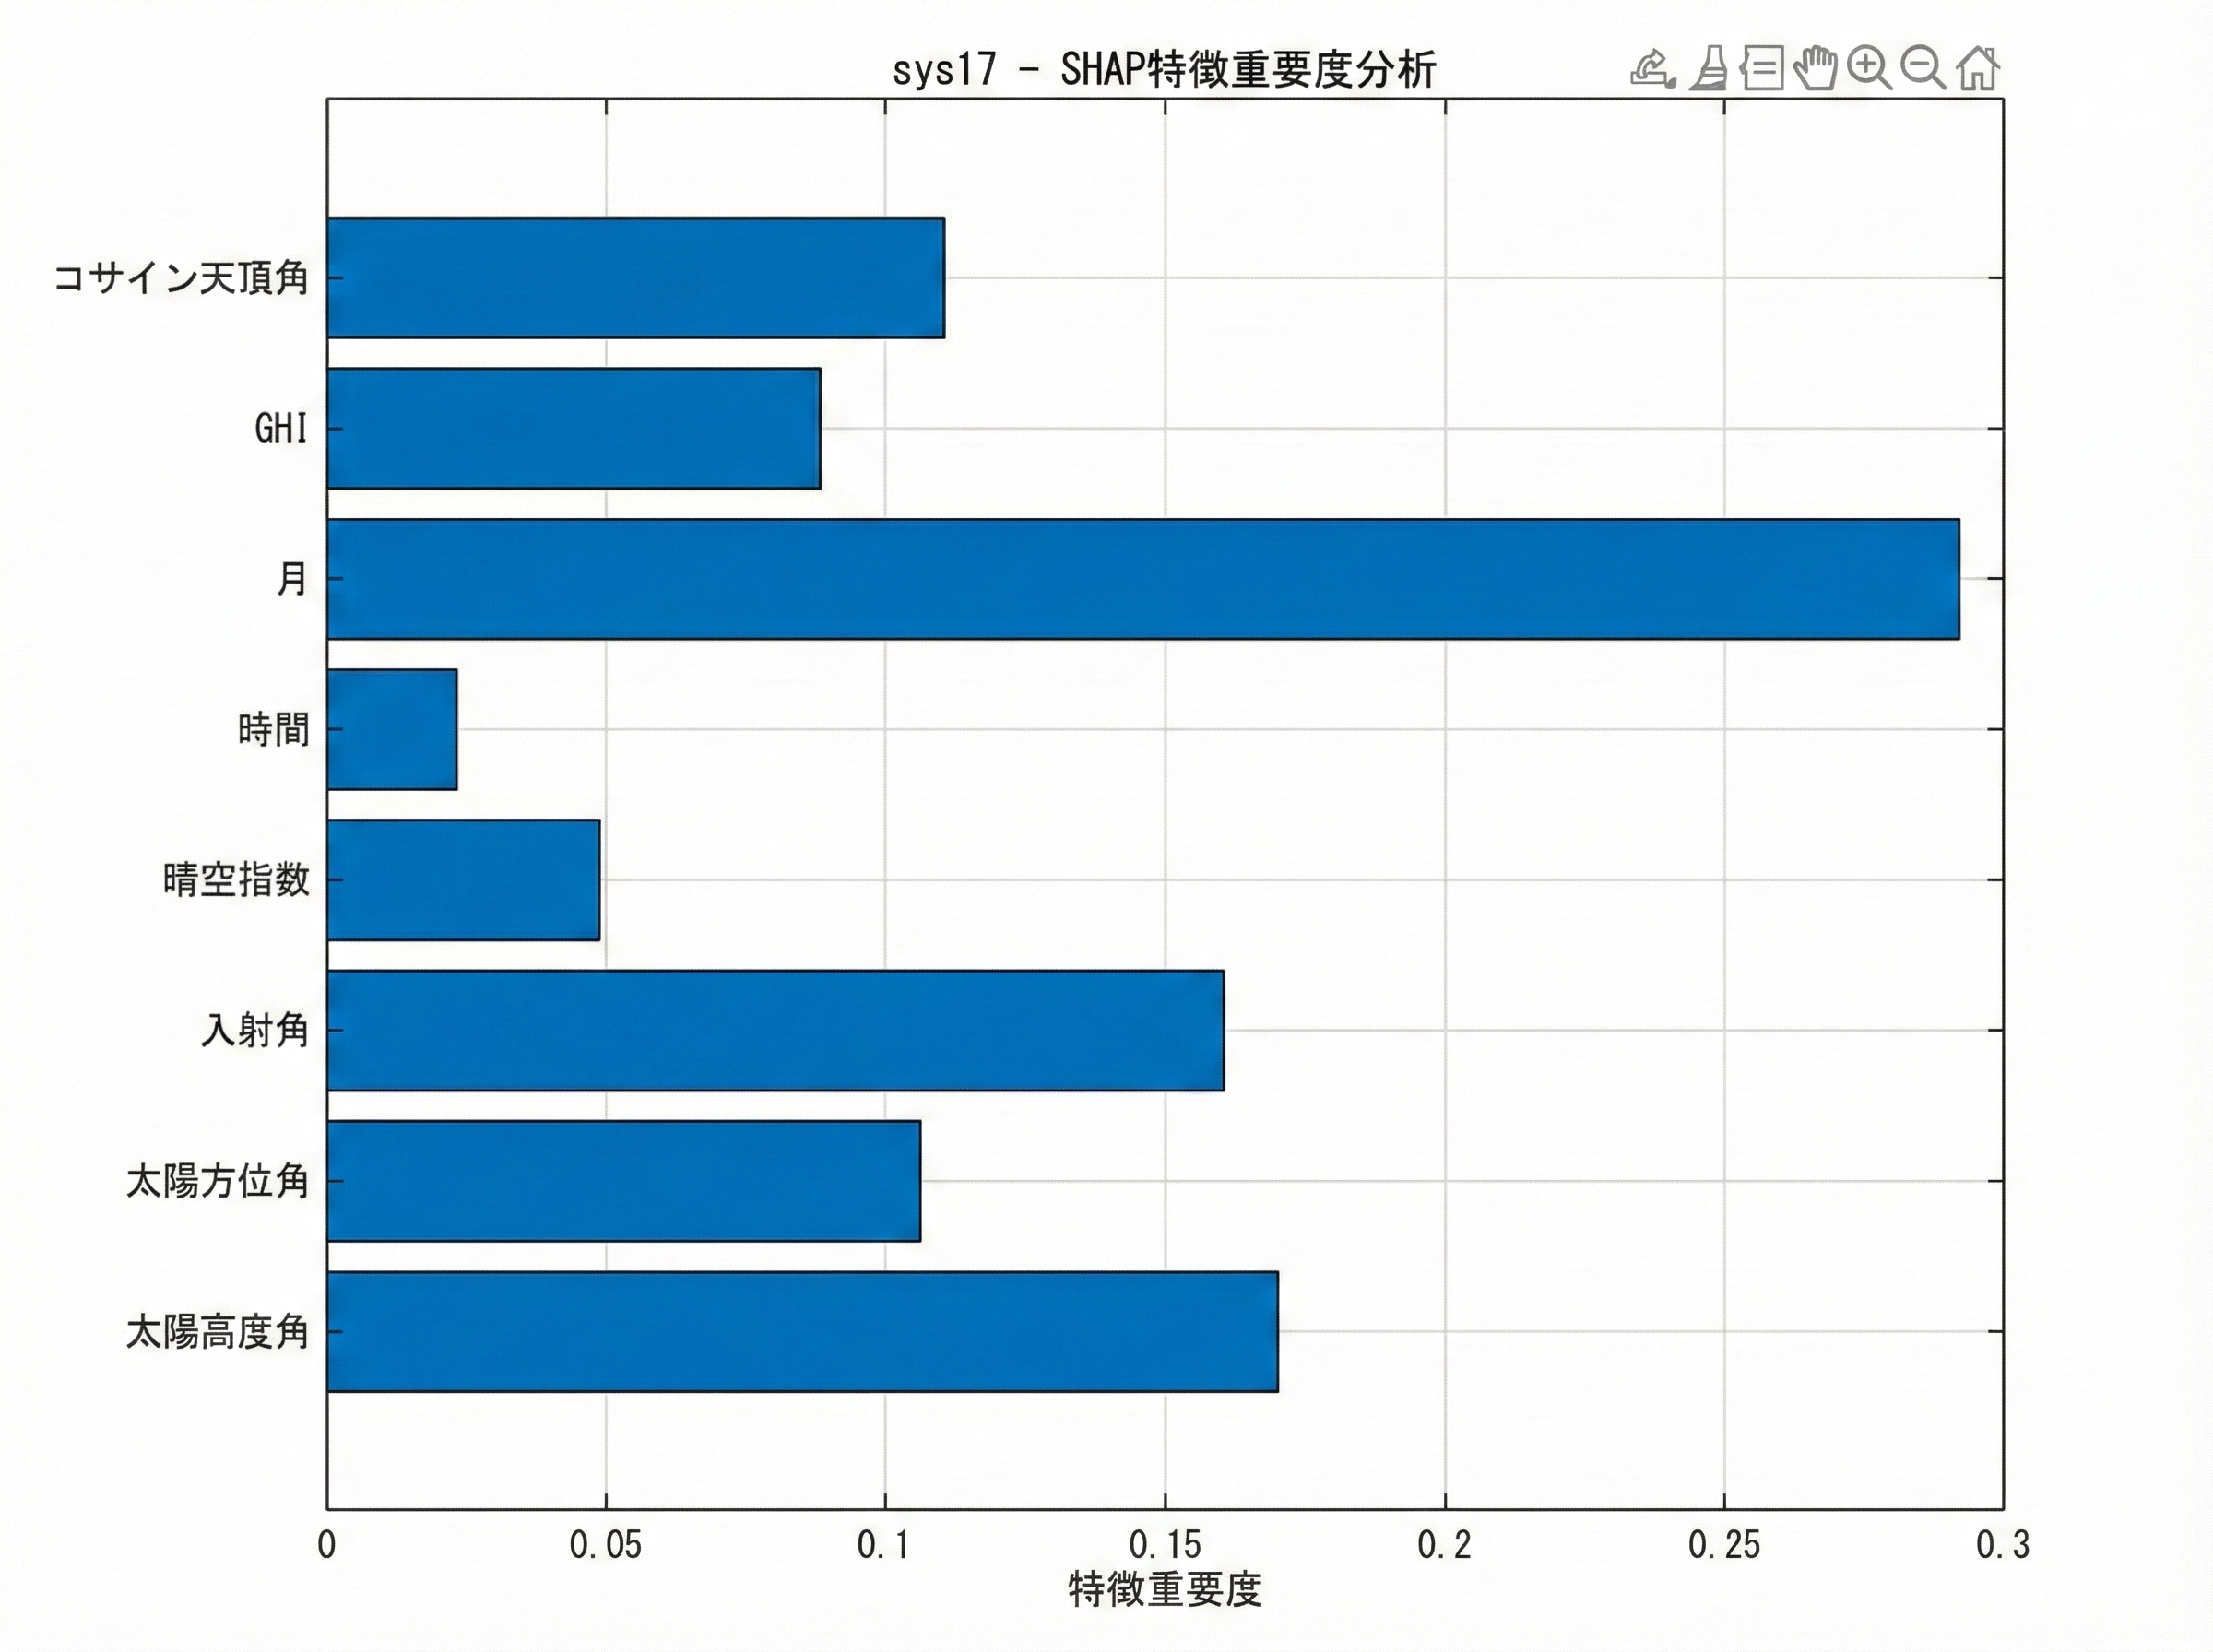
\includegraphics[width=\textwidth]{foto/Hokuto/Sys17SHAPImportanceAnalysis.png}
        \caption*{(b) Sys17(異常系)}
    \end{minipage}
    \caption{SHAP値に基づく特徴量重要度の比較}
    \label{fig:shap_comparison}
\end{figure}
\FloatBarrier

%------------------------------------------------------------------------
\subsection{正常システム(Sys21)の特徴量分布}
\label{subsec:正常システム(Sys21)の特徴量分布}
%------------------------------------------------------------------------

図\ref{fig:shap_comparison}(a)に示すSys21の結果を確認すると、特徴量の重要度が比較的均等に分散していることが分かる。
特に、「月(Month)」、「晴空指数(Clearness Index)」、「GHI(水平面日射量)」、「太陽高度角」がいずれも 0.14 前後の高い値を示している。これは、正常なPVシステムにおいて、発電誤差(残差)の主な要因が、季節による気温変化(月)や、雲の通過によるスペクトル変化(晴空指数・GHI)といった\textbf{「気象的・光学的要因」}によって支配されていることを意味する。特定の幾何学的条件だけに依存しない、自然な物理挙動を示していると言える。

\subsection{異常システム(Sys17)における幾何学的依存性}
一方、図\ref{fig:shap_comparison}(b)に示すSys17の結果は、Sys21とは明確に異なる傾向を示している。

\begin{enumerate}
    \item \textbf{「月」および「幾n何学パラメータ」の突出}: \\
    最も顕著な特徴として、「月(Moth)」の重要度が 0.29 近くまで突出している。次いで「太陽高度角(Solar Altitude)」、「入射角(Incidence Angle)」、「太陽方位角(Solar Azimuth)」といった幾何学的パラメータが高い重要度を示している。
    これは、Sys17の出力低下が、特定の季節(冬期など)および特定の太陽位置においてのみ発生する現象であることをモデルが学習した結果である。

    \item \textbf{水平面日射量(GHI)の重要度低下}: \\
    対照的に、発電量に最も寄与するはずの「GHI」の重要度は 0.1 未満まで低下している。もし出力低下の原因が「局所的な雲」であれば、GHIや晴空指数の重要度が高くなるはずである。しかし、本結果ではGHIよりも太陽の位置情報(高度・方位・入射角)が重視されている。
\end{enumerate}

%------------------------------------------------------------------------
\subsection{時空間マッピングによる遮蔽物の定位}
\label{subsec:時空間マッピングによる遮蔽物の定位}
%------------------------------------------------------------------------

最後に、特定された日陰要因が、物理空間上の「どこ」に存在し、「いつ」影響を及ぼしているかを特定するため、検出された遮蔽パターンの方位角依存性および時間依存性をマッピングする。

図\ref{fig:azimuth_pattern_comparison}に、Sys21およびSys17における太陽方位角ごとの遮蔽率(Shadow Ratio)および残差分布を示す。

正常システムであるSys21(図\ref{fig:azimuth_pattern_comparison}(a), (c))においては、全方位にわたり遮蔽率は低く、残差分布もフラットである。散発的なノイズが見られるものの、特定の方角にピークを持つような構造的特徴は皆無である。

対して、異常システムであるSys17(図\ref{fig:azimuth_pattern_comparison}(b), (d))では、明確な指向性が確認された。

\begin{enumerate}
    \item \textbf{遮蔽率の鋭いピーク}: 方位角 $0^\circ$(真南)から $+20^\circ$(南西)の範囲において、遮蔽率が最大 0.7(70\%)に達する鋭いピークが形成されている。
    \item \textbf{残差のV字急落}: 散布図(d)においても、同方位角範囲にて残差が急激に負の方向へ落ち込むV字型のパターンが明瞭に現れている。
\end{enumerate}

このデータは、Sys17から見て「南〜南西」の方向に、発電を著しく阻害する物理的な遮蔽物が存在することを示している。

\begin{figure}[htbp]
    \centering
    \begin{minipage}[b]{0.48\textwidth}
        \centering
        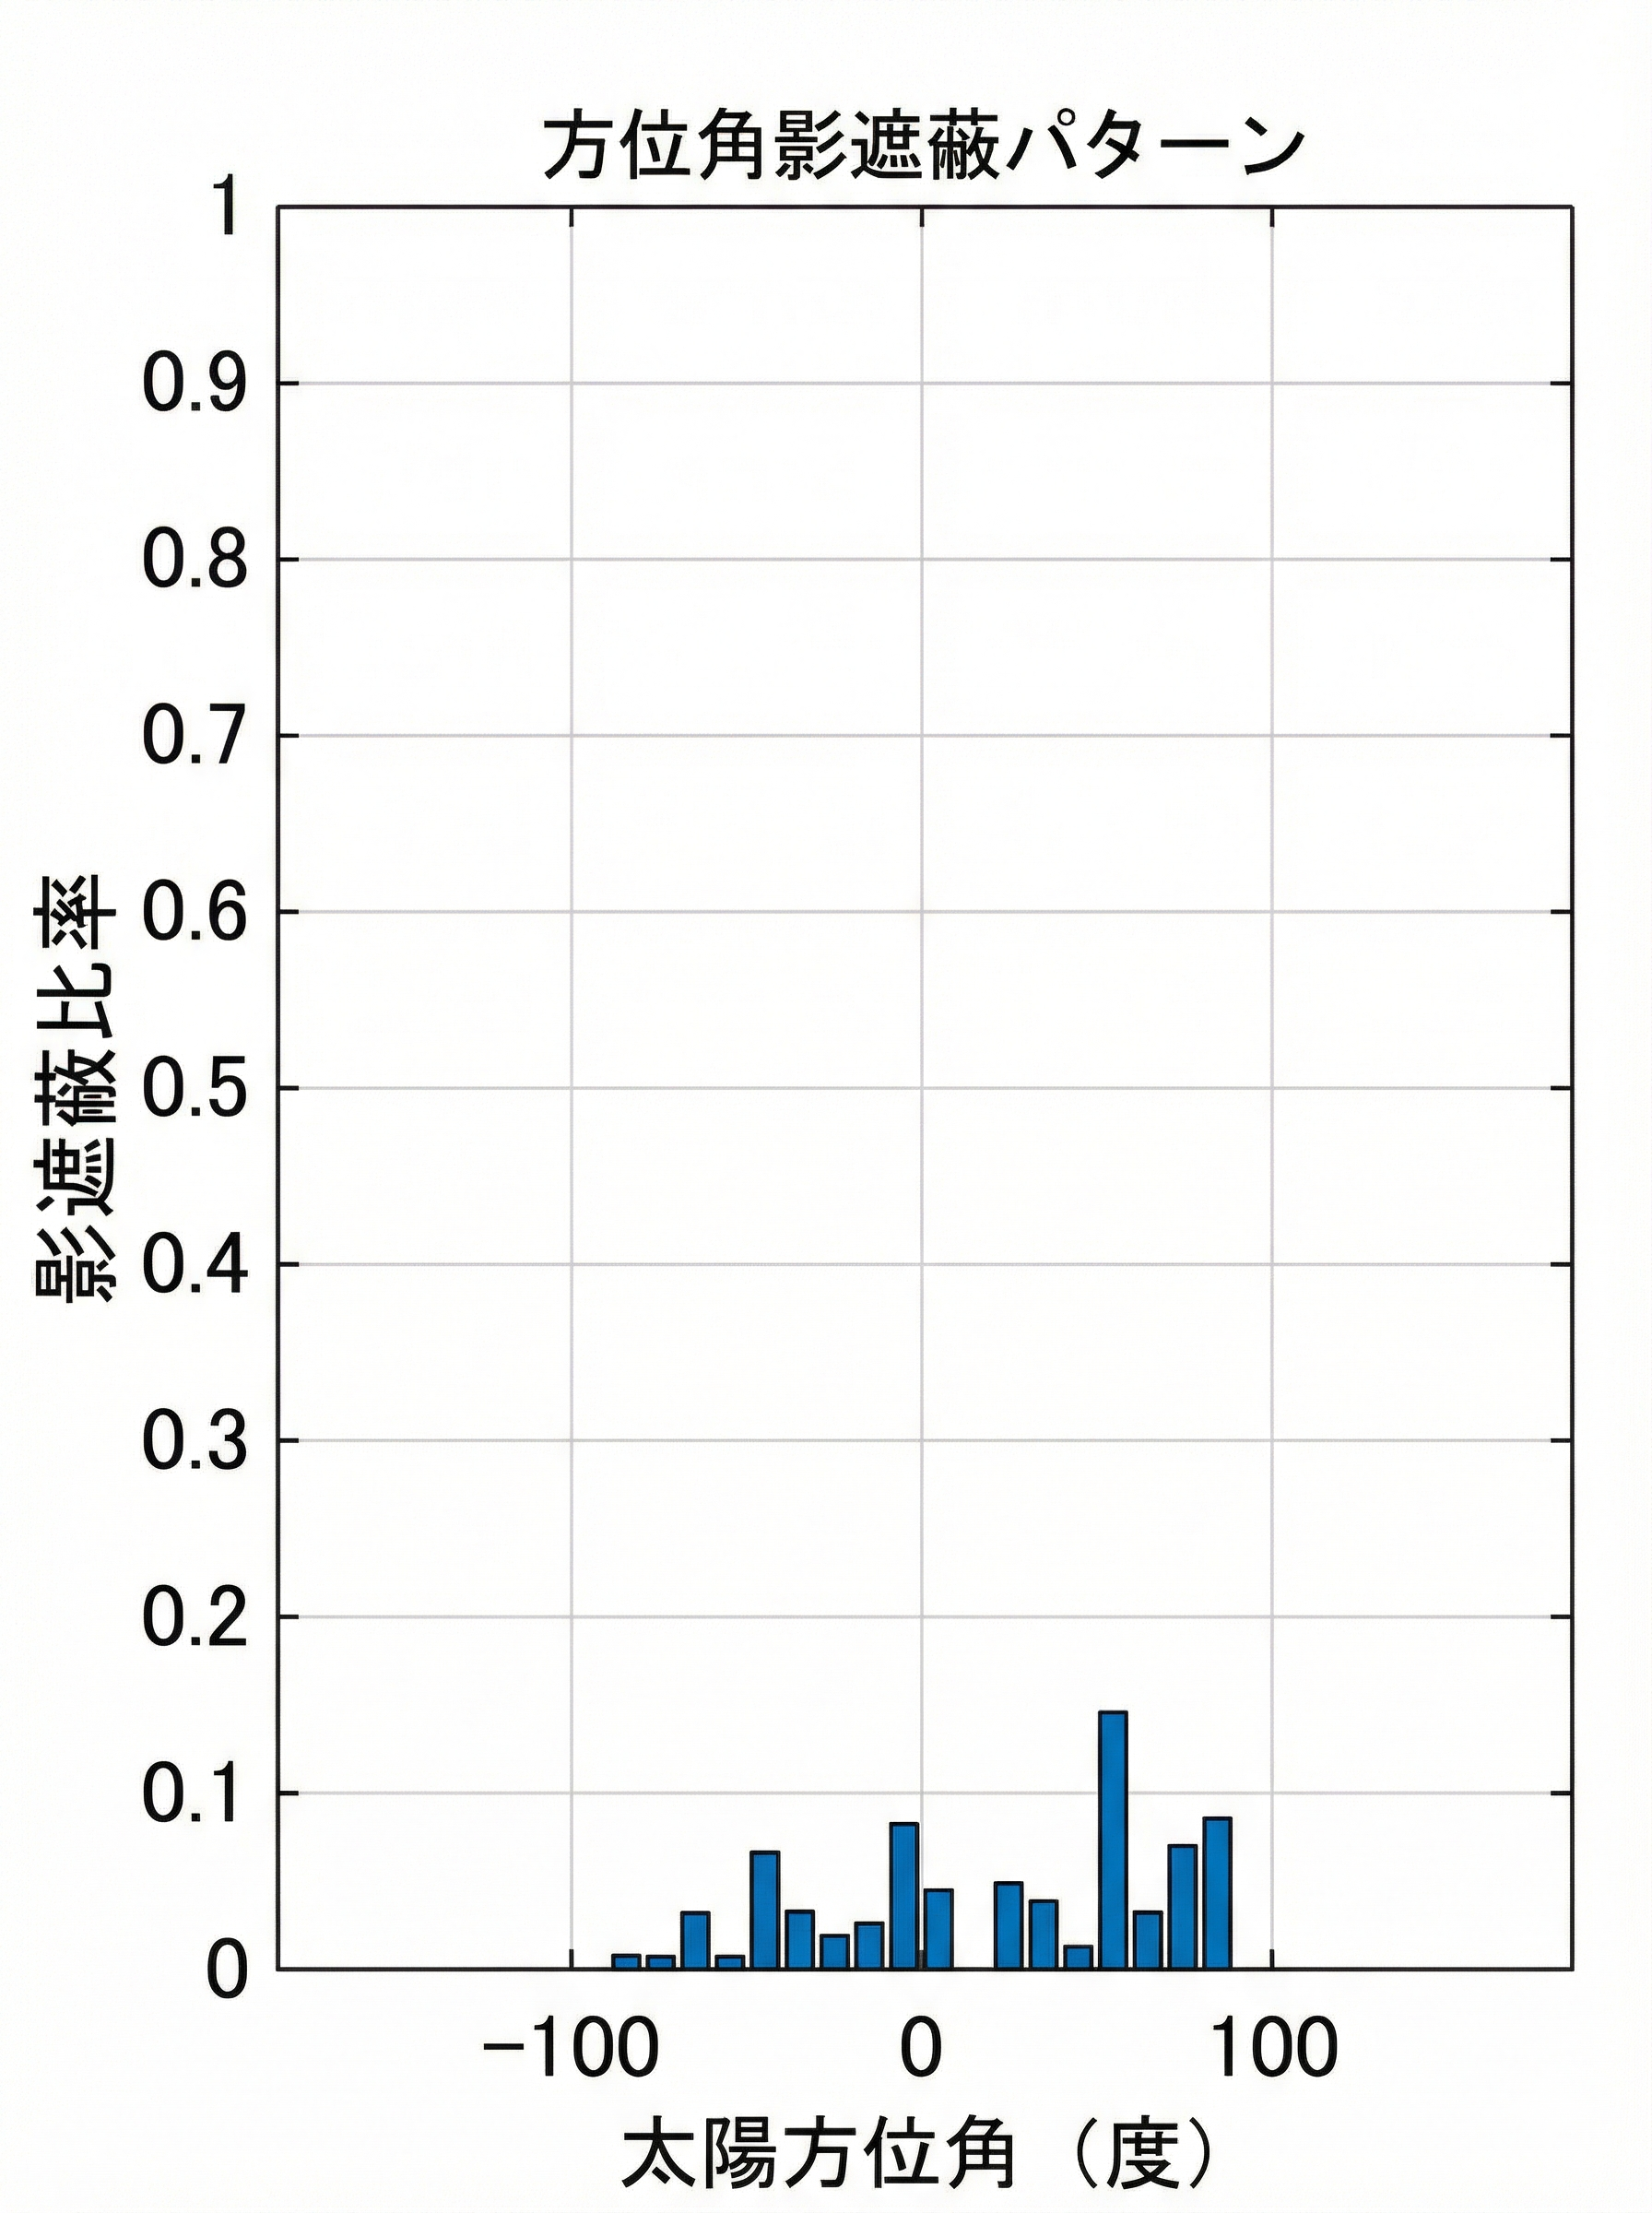
\includegraphics[width=\textwidth]{foto/Hokuto/Sys21AzimuthShadowOcclusionPattern.png}
        \caption*{(a) Sys21: 方位角遮蔽率(正常)}
    \end{minipage}
    \hfill
    \begin{minipage}[b]{0.48\textwidth}
        \centering
        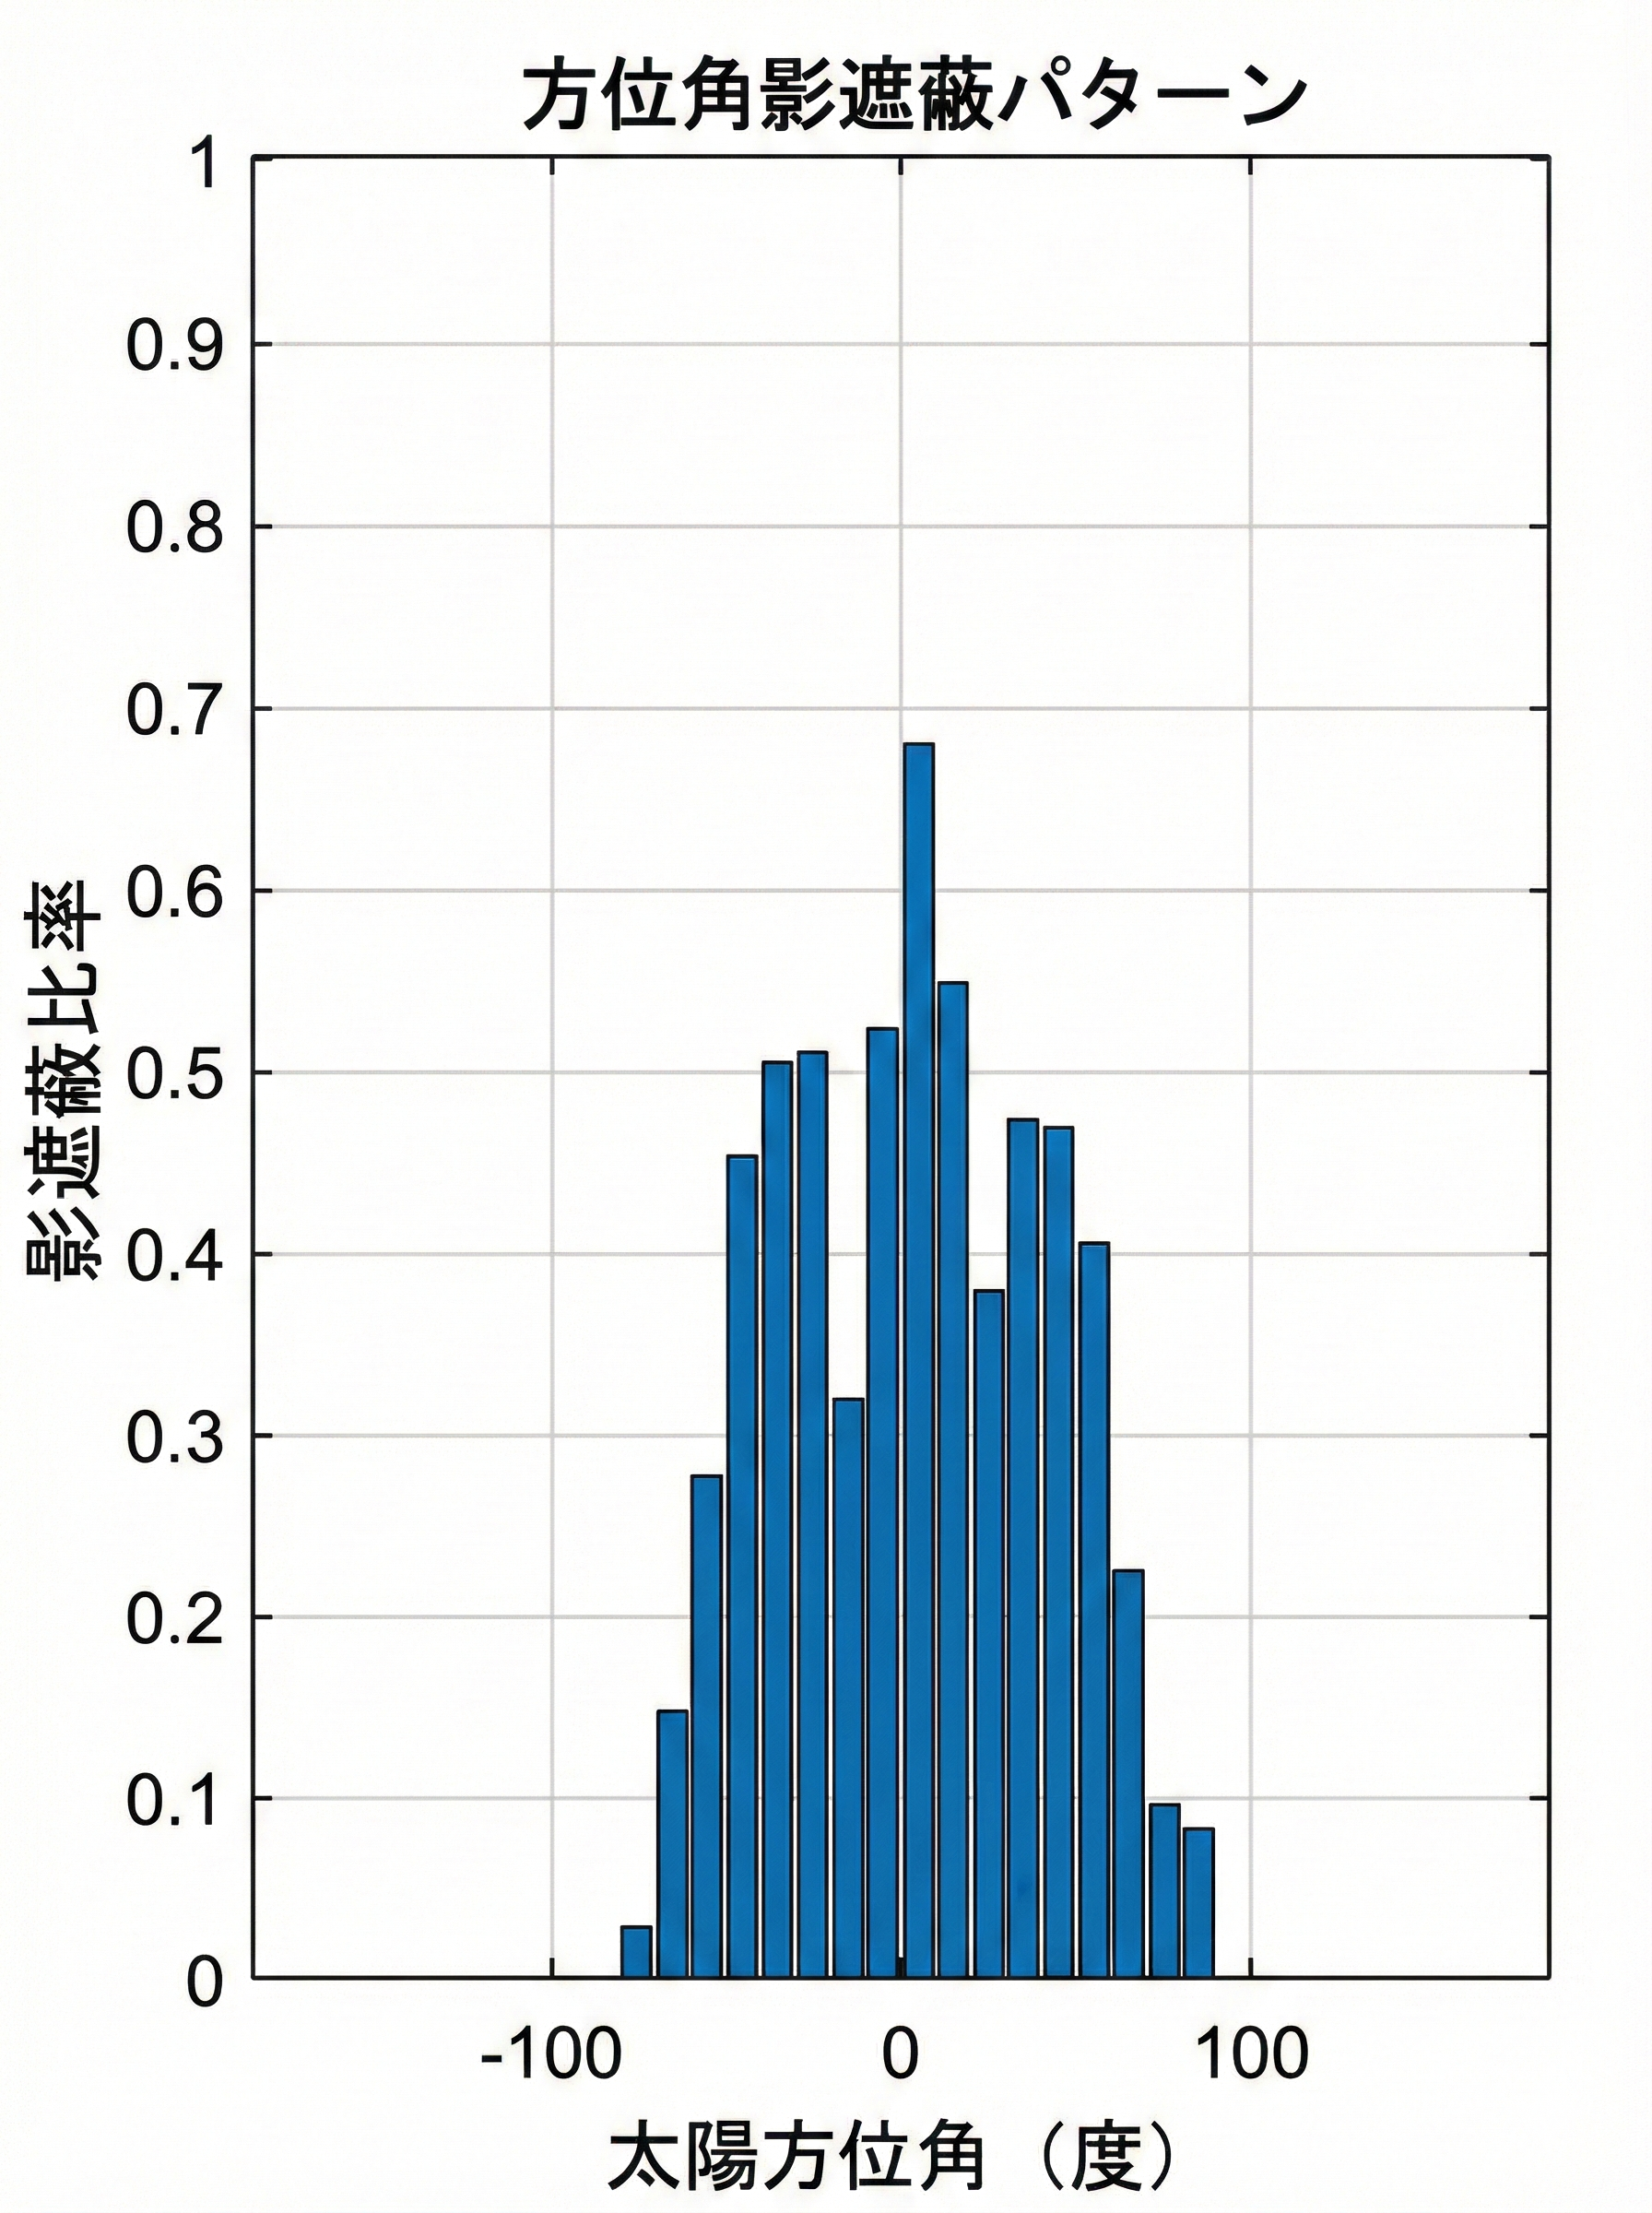
\includegraphics[width=\textwidth]{foto/Hokuto/Sys17AzimuthShadowOcclusionPattern.png}
        \caption*{(b) Sys17: 方位角遮蔽率(異常)}
    \end{minipage}
    \vspace{0.5cm}
    \begin{minipage}[b]{0.48\textwidth}
        \centering
        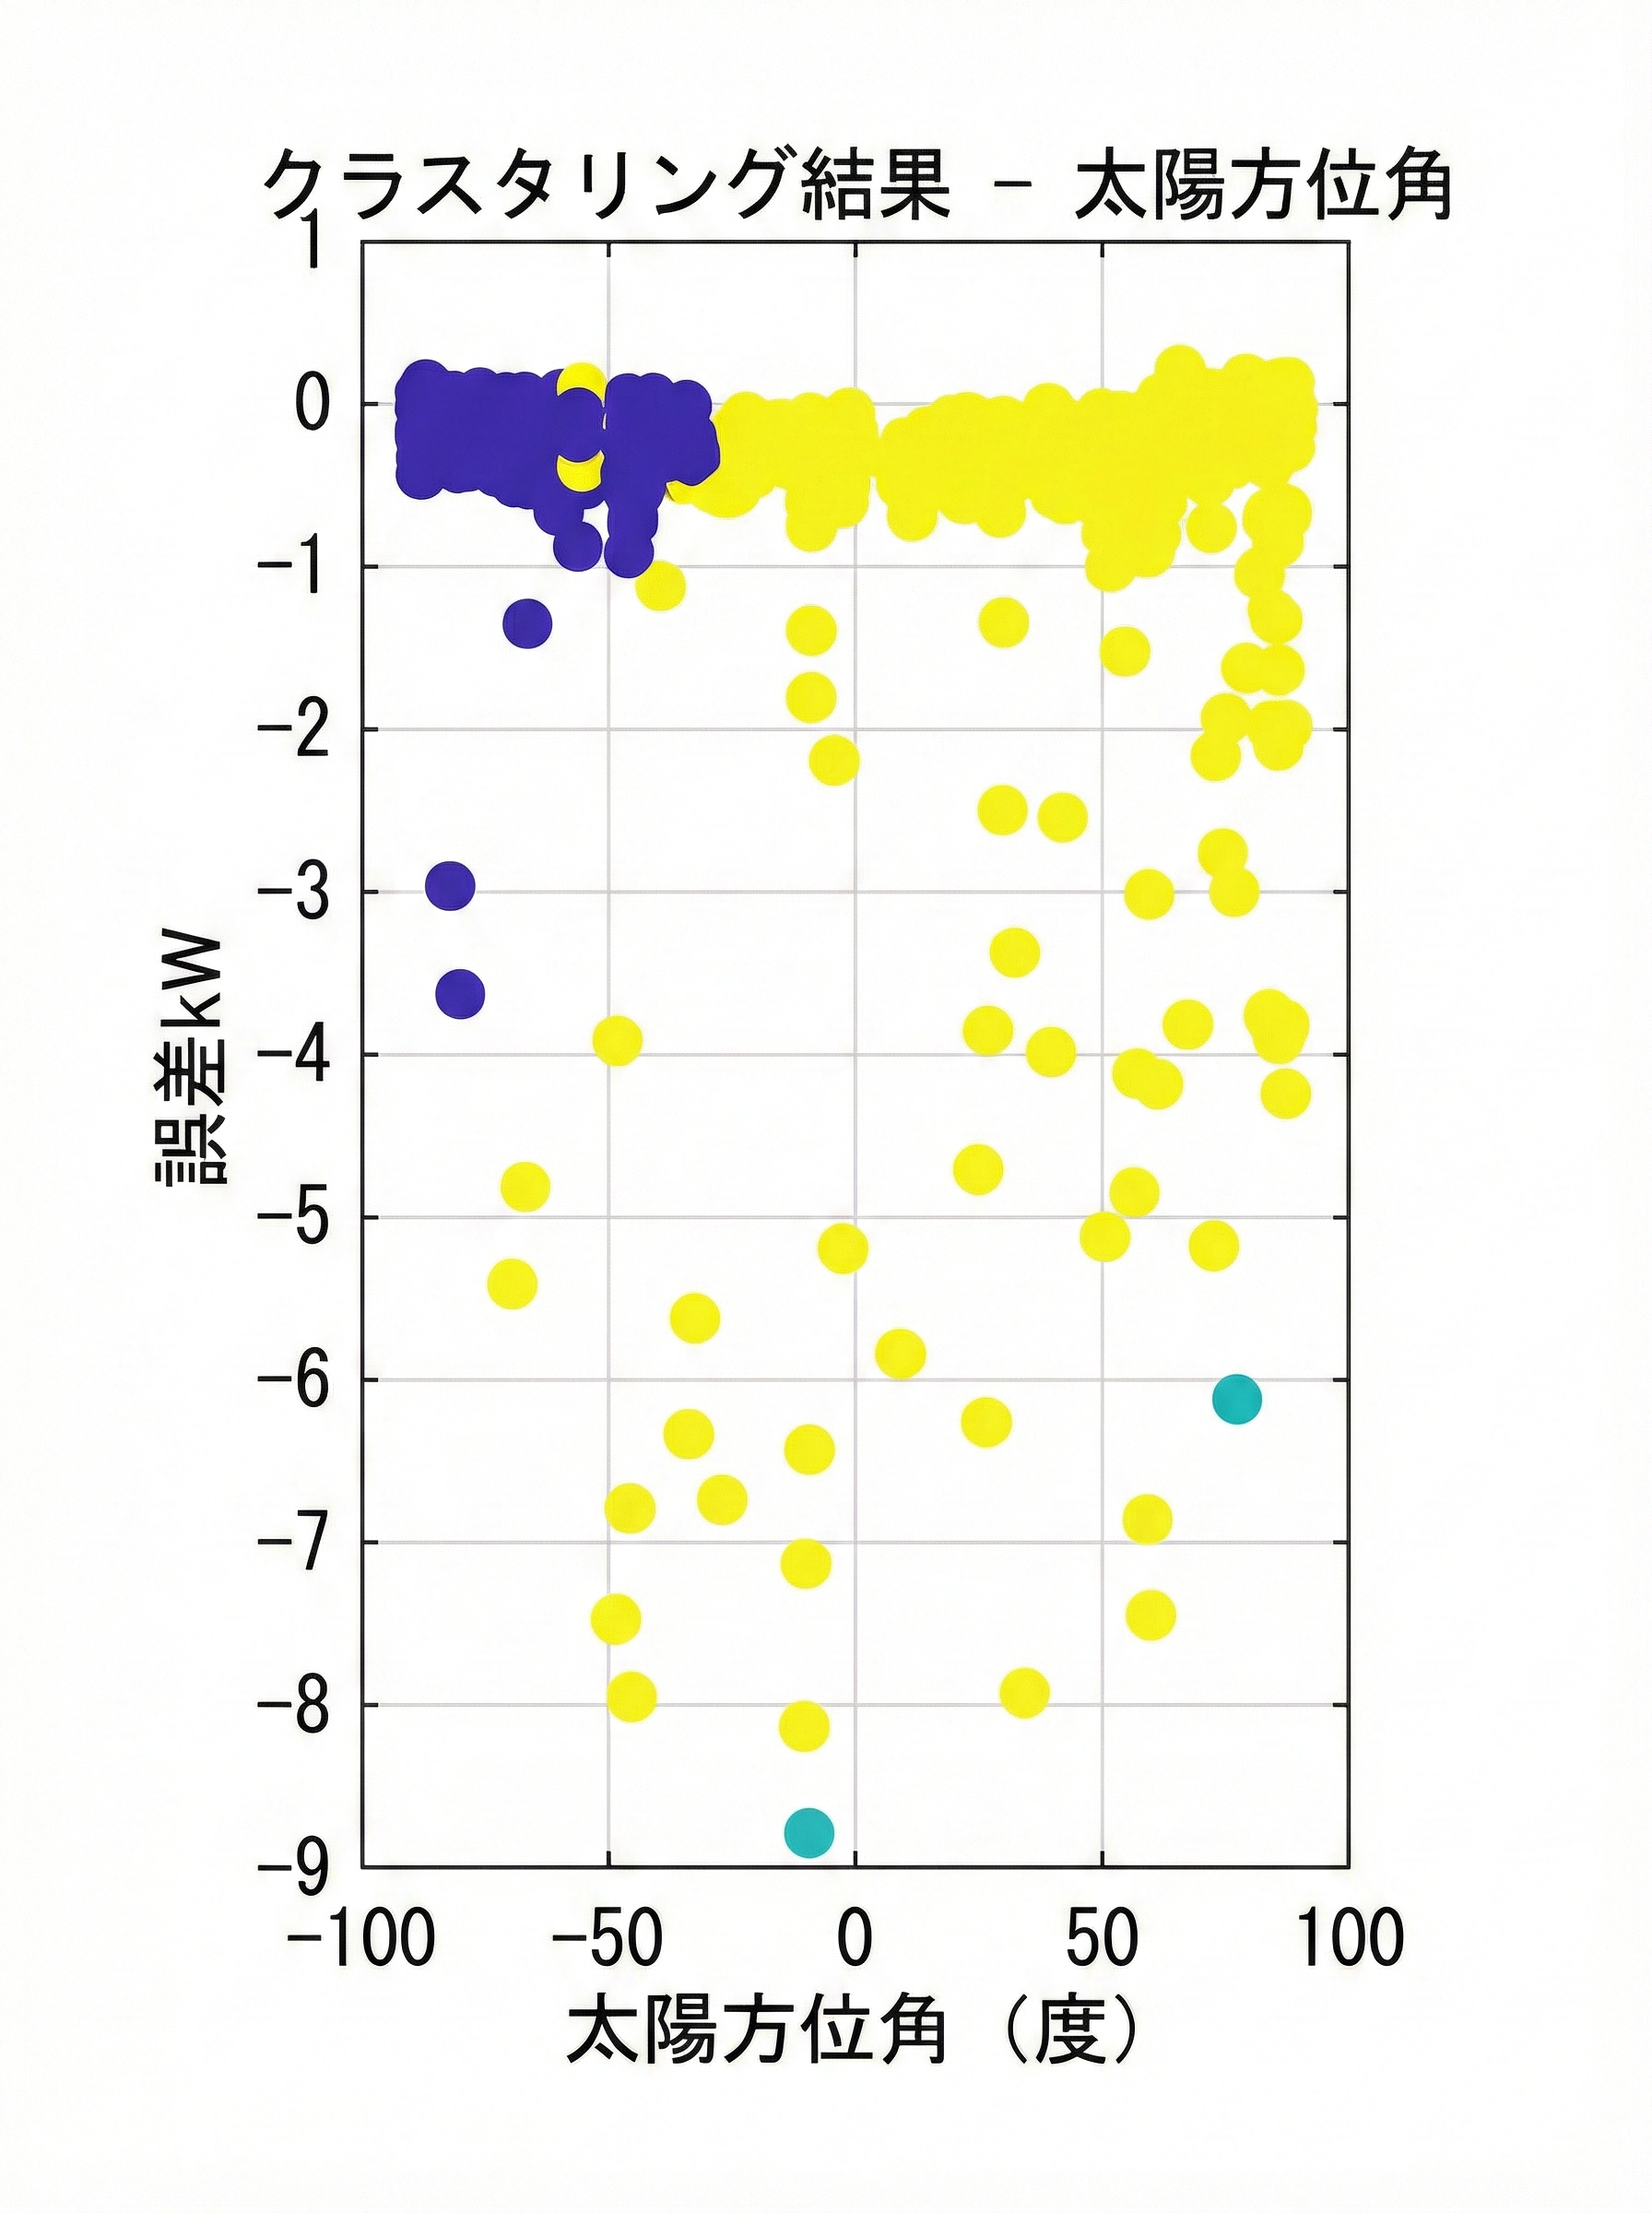
\includegraphics[width=\textwidth]{foto/Hokuto/Sys21ClusteringResultsSolarAzimuthAngleAndError.png}
        \caption*{(c) Sys21: 方位角残差散布}
    \end{minipage}
    \hfill
    \begin{minipage}[b]{0.48\textwidth}
        \centering
        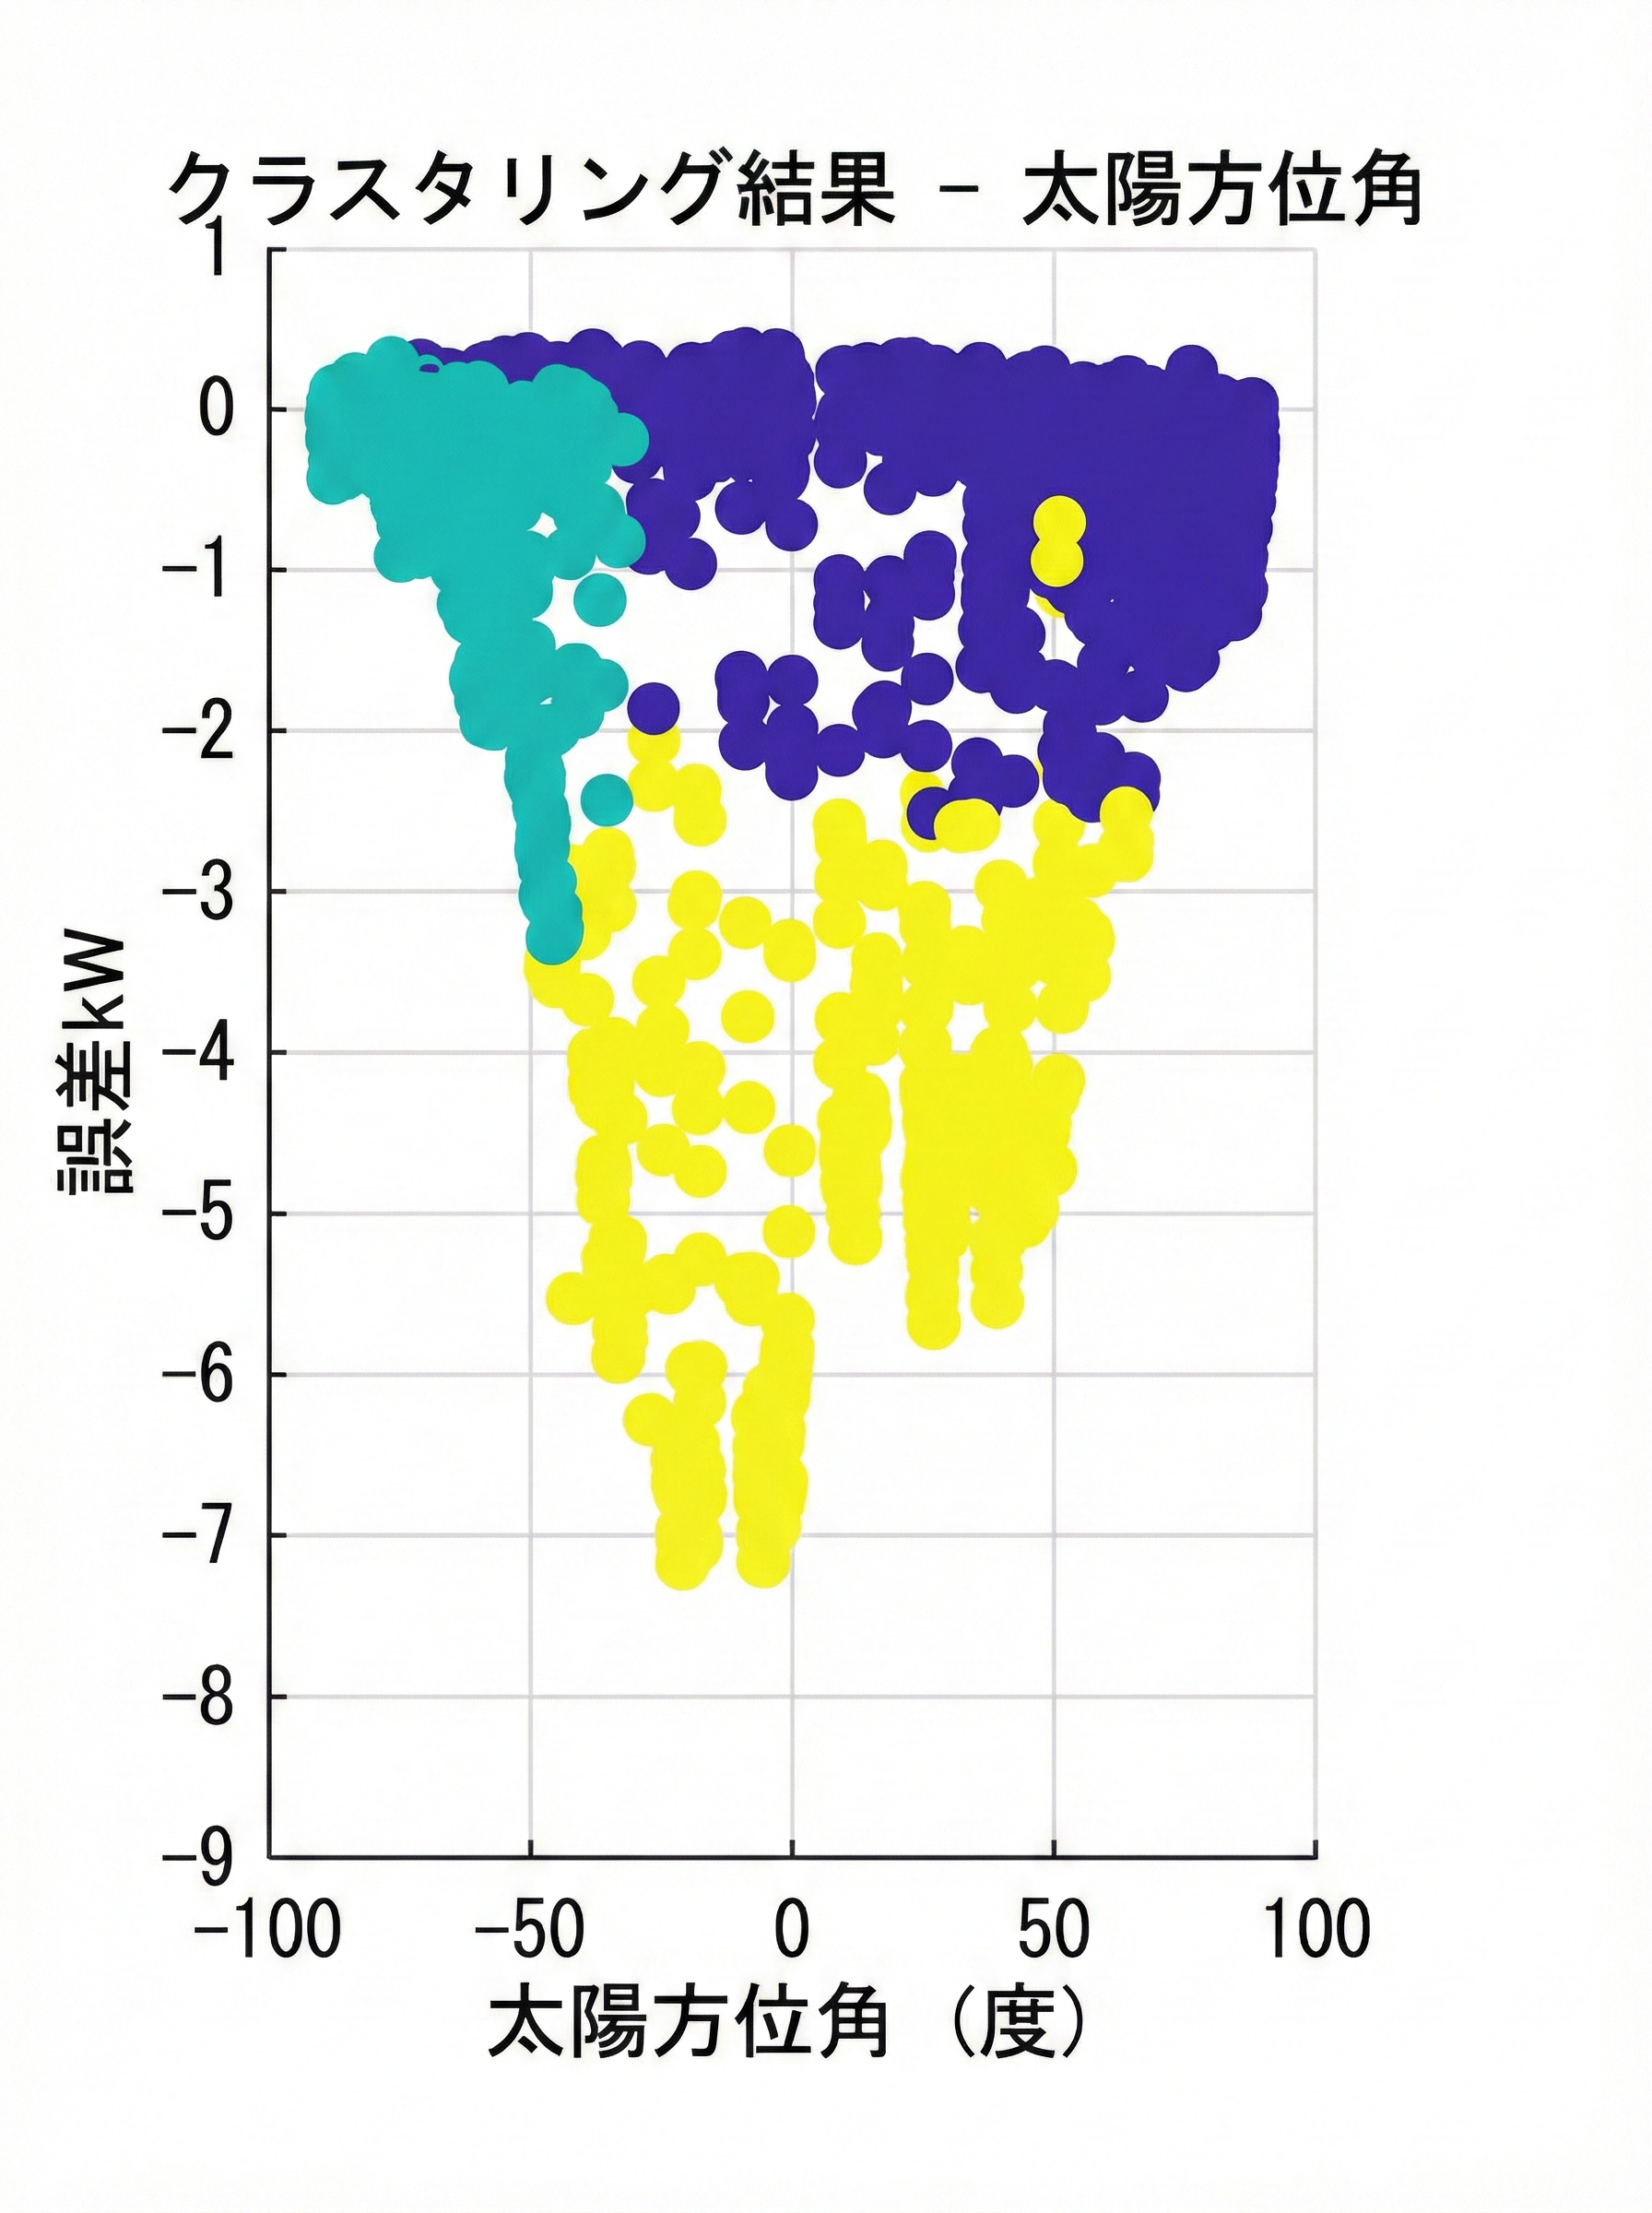
\includegraphics[width=\textwidth]{foto/Hokuto/Sys17ClusteringResultsSolarAzimuthAngleAndError.png}
        \caption*{(d) Sys17: 方位角残差散布}
    \end{minipage}
    \caption{太陽方位角に基づく遮蔽パターンの比較(南西方向の異常検出)}
    \label{fig:azimuth_pattern_comparison}
\end{figure}
\FloatBarrier

図\ref{fig:time_pattern_comparison}に、時刻別の遮蔽率推移を示す。

Sys21(a)の遮蔽率は一日を通じて 0.1 未満で推移しており、突発的な雲の影響を除けば安定している。

一方、Sys17(b)では、日中の広範囲で高い遮蔽率を示しているが、特筆すべきは \textbf{14:00(午後2時)} に見られる顕著なピークである。この時刻は、太陽が南中を過ぎて西に傾き始めるタイミングであり、前述した南西方向の遮蔽物と幾何学的に整合する。

\begin{figure}[htbp]
    \centering
    \begin{minipage}[b]{0.48\textwidth}
        \centering
        \includegraphics[width=\textwidth]{foto/Hokuto/Sys21ShadowOcculusionPatternByTime.png}
        \caption*{(a) Sys21: 時間別遮蔽率}
    \end{minipage}
    \hfill
    \begin{minipage}[b]{0.48\textwidth}
        \centering
        \includegraphics[width=\textwidth]{foto/Hokuto/Sys17ShadowOcculusionPatternByTime.png}
        \caption*{(b) Sys17: 時間別遮蔽率}
    \end{minipage}
    \caption{時刻別遮蔽パターンの比較}
    \label{fig:time_pattern_comparison}
\end{figure}
\FloatBarrier

以上の解析により、Sys17の出力低下要因は「南〜南西方向に位置する遮蔽物」により「午後(特に14時前後)」に発生する定常日陰であると特定された。

この解析結果を、第\ref{sec:解析対象地点の概要}項で示した現地の航空写真と照合すると、発電パネルの南西方向に隣接する森林の位置と完全に一致することが確認できる。

本結果は、提案手法が設備図面や現地調査といった事前情報を一切使用せず、発電データと一般的な気象データのみから、障害物の有無・方向・影響時間を高い精度で逆推定可能であることを証明するものである。

%************************************************************************
\section{手法の汎用性検討}
\label{subsec:手法の汎用性検討}
%************************************************************************

本節では、第3章で定義したデータセットB(茨城県)を用い、提案手法の汎用性とロバスト性を検証する。データセットA(北杜市)が理想的な計測環境であったのに対し、データセットBは以下のような実用上の厳しい制約条件を有している。

\begin{enumerate}
    \item \textbf{計測データの欠落}: 
    発電電力($P_{meas}$)のみが提供されており、直流電圧($V_{DC}$)およびモジュール温度($T_{mod}$)の計測データが存在しない。このため、第\ref{chapter:モデルの構築 (Methodology)} 章で提案した電圧依存の機械学習モデルや、温度補正項 $\gamma(T_c - 25)$ を物理モデルに直接適用することが不可能である。

    \item \textbf{地理的分散と参照データの物理的乖離}: 
    解析対象となる各PVシステムは互いに地理的に離れた場所に分散しており、気象条件が均一ではない。また、参照データとして用いる静止気象衛星(ひまわり8号)のデータは、トップオブアトモスフェア(TOA)付近の\textbf{短波放射量(Shortwave Radiation: SWR)}に基づき推定されたものであり、地上で日射計により観測される全天日射量(GHI)とは物理的な定義やスペクトル特性が異なる。加えて、衛星データは一定のグリッド解像度(5km平方)における\textbf{空間平均値}であるため、地上の一点における局所的な水平面日射量とは本質的に異なる特性を持つ。

    \item \textbf{設置環境の多様性と外乱要因}: 
    統一された規格を持つデータセットAとは異なり、各システムの設備容量には大きな開き(11kW $\sim$ 44kW)があり、設置方位・傾斜角も多岐にわたる。さらに、住宅地域や市街地に設置されているため、近隣の高層建築物や塔屋に由来する遠方からの不規則な影(ランダムな遮蔽)の影響を受けやすい。また、長期間にわたりパネル洗浄等のメンテナンスが行われていないことに起因する汚れの蓄積など、制御不能な環境外乱が含まれている。
\end{enumerate}

これらの制約下において、提案モデルがいかにして物理的な整合性を保ち、日射量を逆推定できるかを評価する。

%------------------------------------------------------------------------
\subsection{制限付きデータ環境におけるモデルの適応と損失係数の挙動}
\label{sec:制限付きデータ環境におけるモデルの適応と損失係数の挙動}
%------------------------------------------------------------------------

温度および電圧データが欠落している場合、物理モデルにおける温度損失や回路損失を個別の項として算出することはできない。そこで本研究では、これらの変動要因をすべて包括的なシステム性能係数 $L_{sys}$(Dataset Aにおける $K_O$ に相当)に吸収させるアプローチをとった。

太陽光発電の場合、温度損失の影響が大きいことを知り、以下、温度の影響の受け方が異なる2つのシステムについて、損失係数の分析結果を述べる。

\textbf{熱損失の影響が軽微な事例(Sys54)}

図\ref{fig:sys54_lsys}に、比較的安定した挙動を示すシステム(Sys54)における $L_{sys}$ の時空間マップおよび経年トレンドを示す。

損失係数ヒートマップ(左図)を確認すると、春季から秋季にかけて高い値(赤色:0.85程度)で安定しており、特定の季節による落ち込みが見られない。また、経年トレンド(右図)においても、2015年から2020年まで月ごとの変動幅が小さく、ほぼフラットな特性を維持している。

これは、当該システムの設置環境(通気性など)が良好と考え、夏季の温度上昇による効率低下が限定的であるため、パラメータ $L_{sys}$ が純粋なシステム効率として一定値を保っていることを示唆している。

\begin{figure}[htbp]
    \centering
    \begin{minipage}[b]{0.48\textwidth}
        \centering
         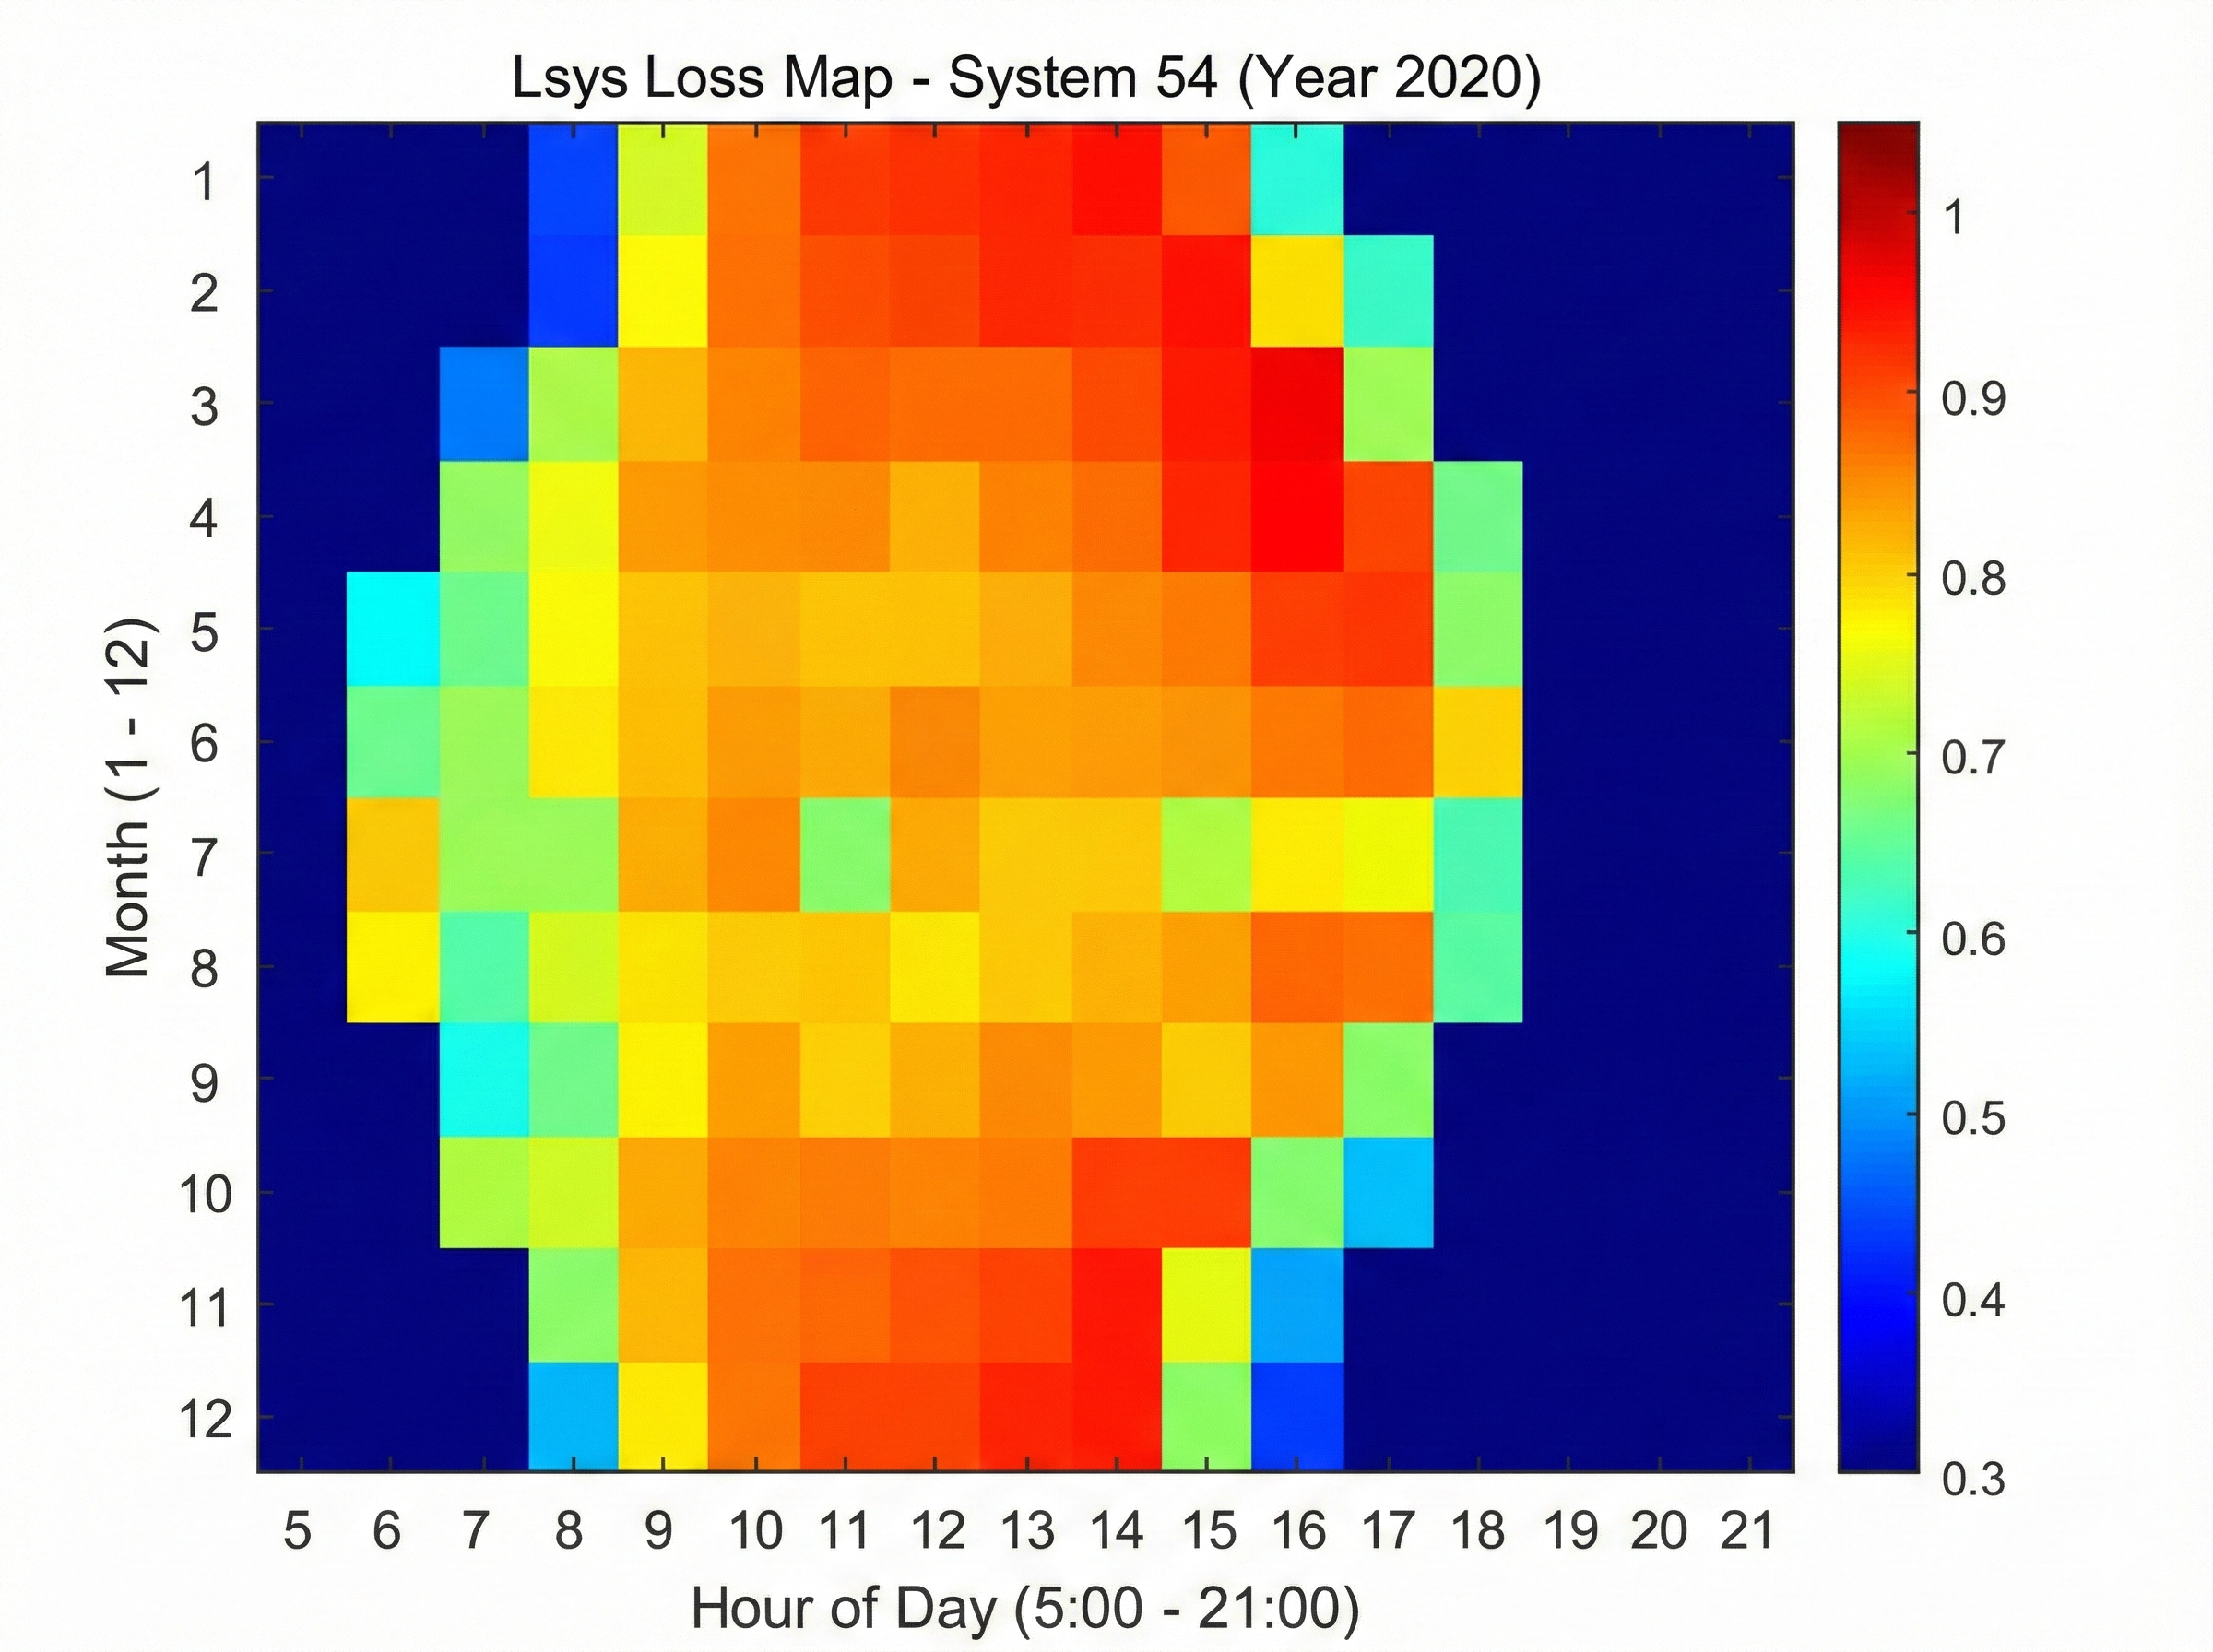
\includegraphics[width=\textwidth]{foto/Ibaraki/Sys54LsysMapRelativelyStable.png}
        \caption*{ (a) 損失係数ヒートマップ }
    \end{minipage}
    \hfill
    \begin{minipage}[b]{0.48\textwidth}
         \centering
        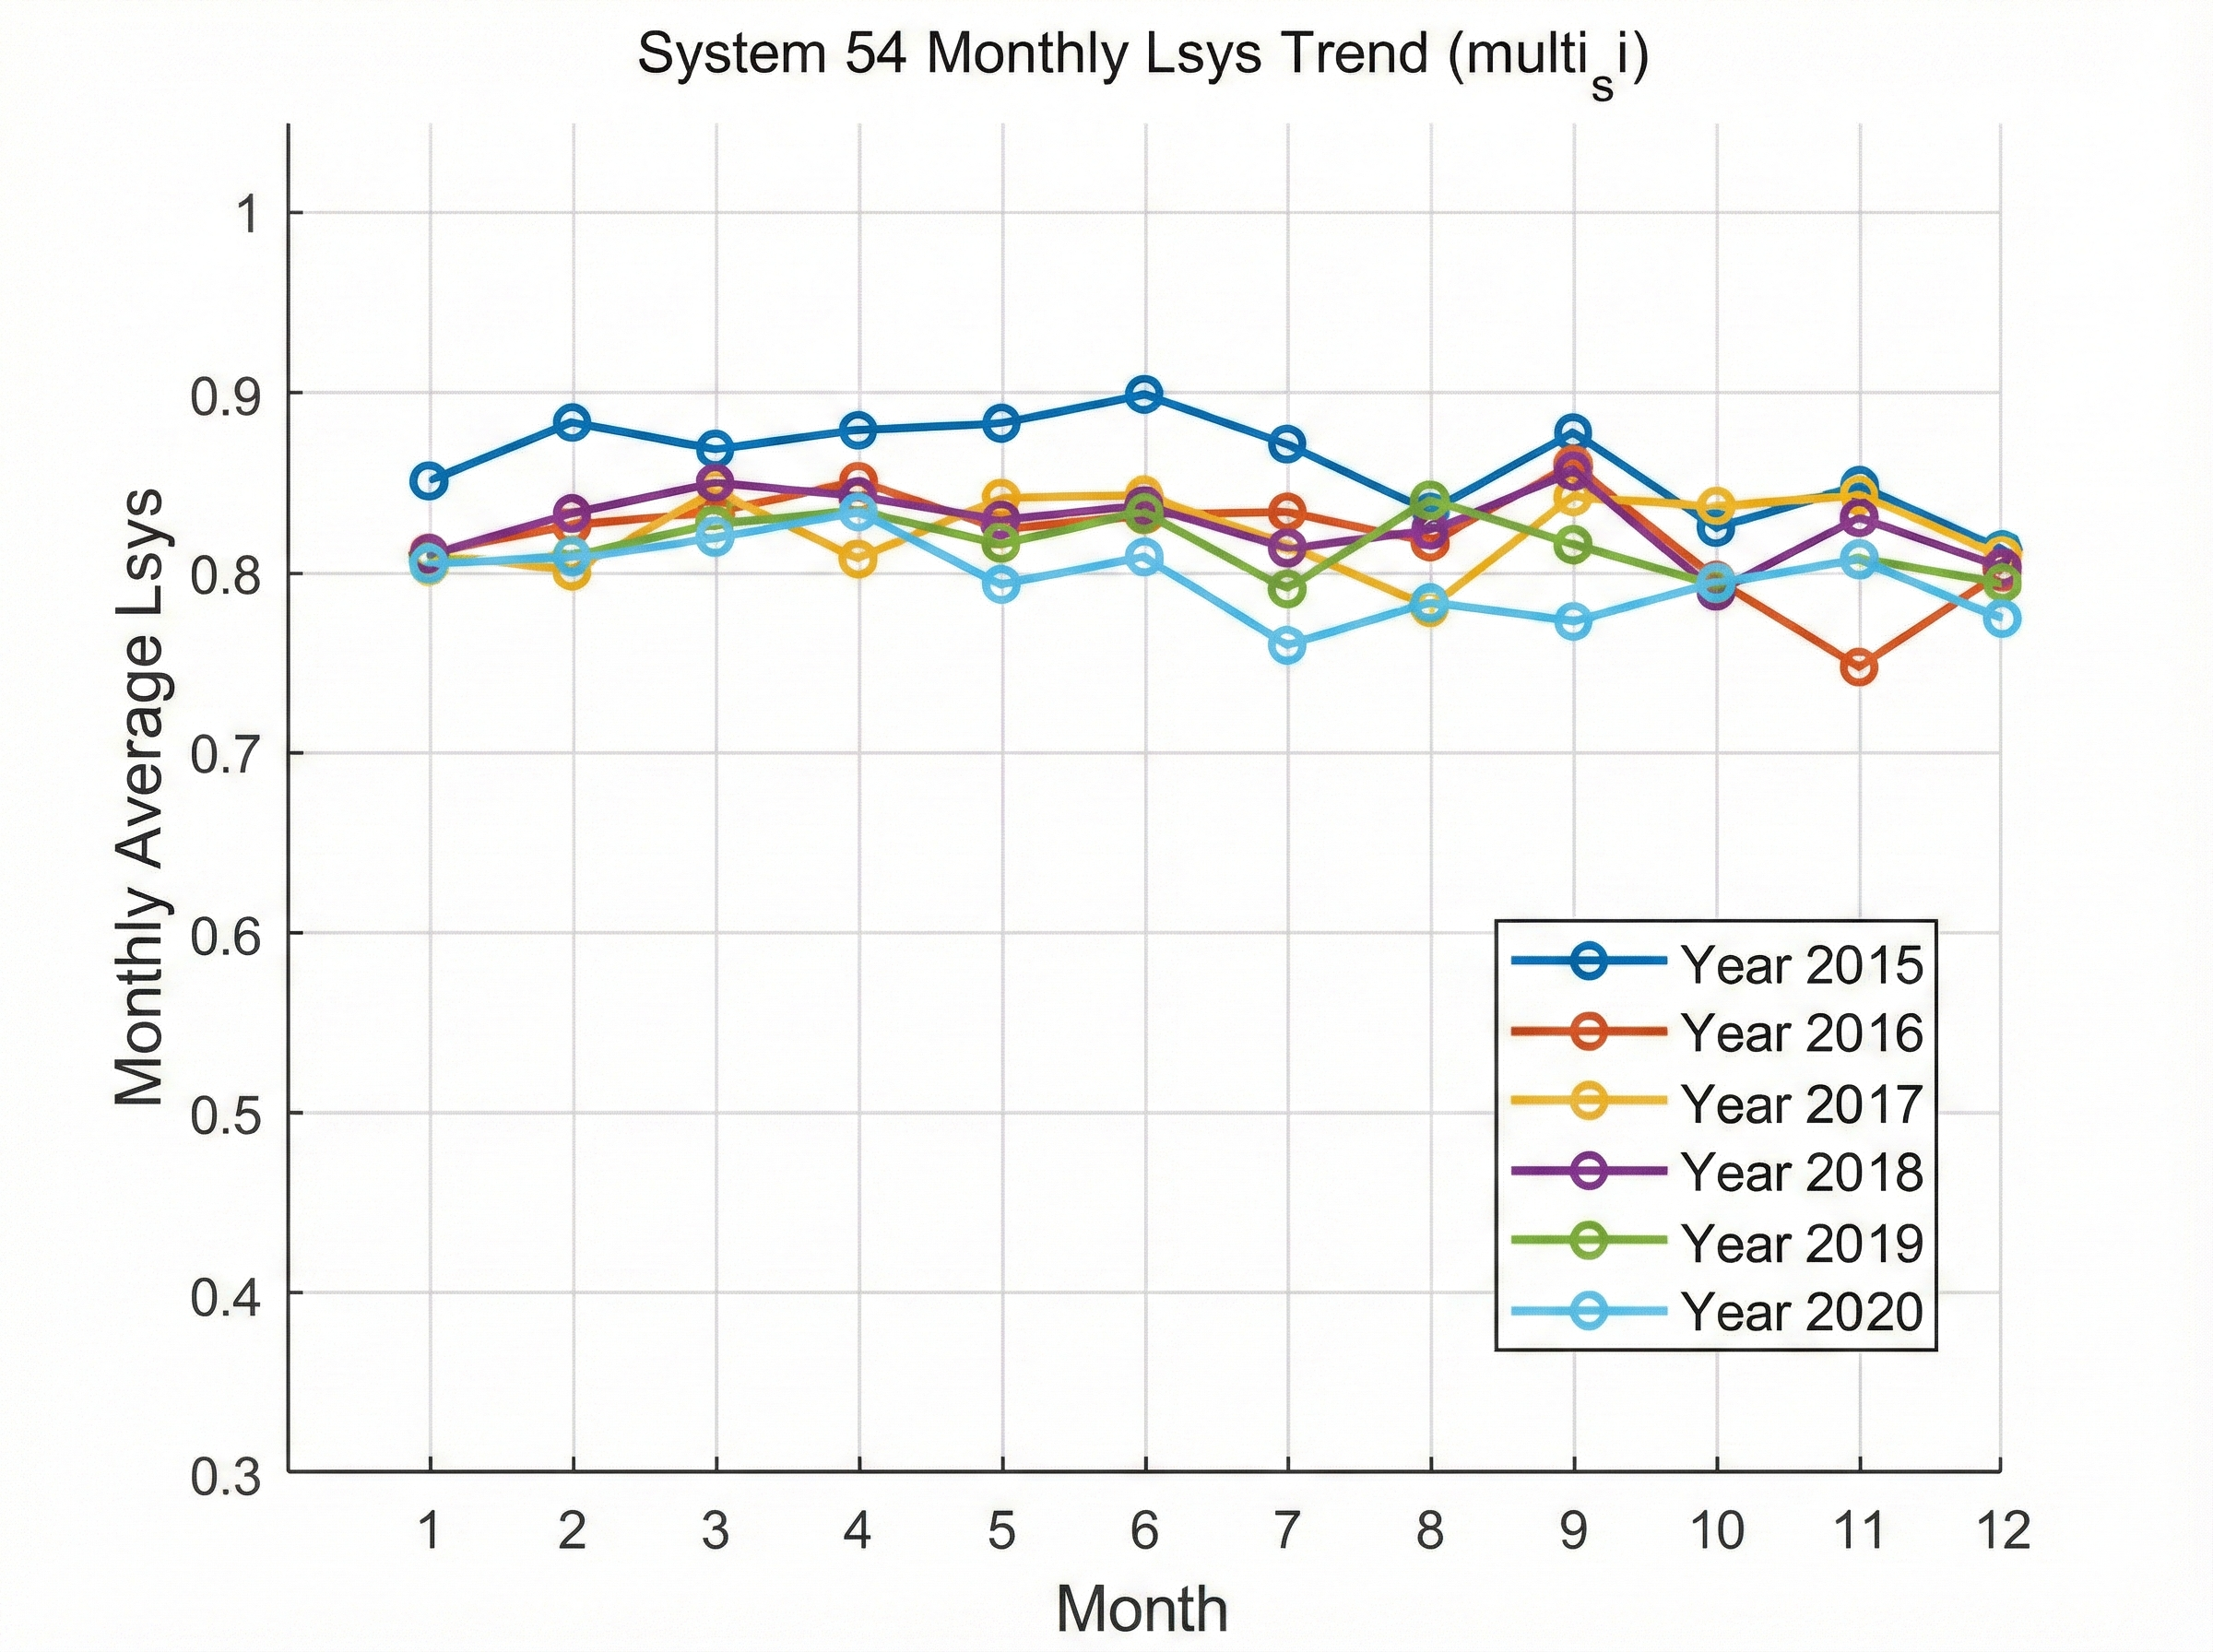
\includegraphics[width=\textwidth]{foto/Ibaraki/Sys54LsysTrendRelativelyStable.png}
        \caption*{ (b) 月別経年トレンド }
    \end{minipage}
    \caption{Sys54における損失係数 $L_{sys}$ の安定した挙動(熱影響小)}
    \label{fig:sys54_lsys}
\end{figure}
\FloatBarrier

\textbf{熱損失をパラメータが吸収した事例(Sys81)}

対照的に、図\ref{fig:sys81_lsys}に、夏季に特徴的な挙動を示すシステム(Sys81)の解析結果を示す。

損失係数ヒートマップ(左図)では、6月から8月の日中時間帯において、係数値が顕著に低下(黄色〜緑色:0.7程度)している領域が確認できる。

さらに経年トレンド(右図)を見ると、多くの年(特に2018年、紫色線)において、夏場(6月〜8月)にグラフが大きく凹む「U字型」の推移を示している。本来、物理モデルに温度項が含まれていれば、この効率低下は温度補正によって相殺されるはずである。

この結果は、提案手法がセンサー不足という悪条件を、統計パラメータの動的な調整によって補い、物理現象(熱損失)を数学的に吸収・表現できていることを証明するものである。

\begin{figure}[htbp]
    \centering
    \begin{minipage}[b]{0.48\textwidth}
        \centering
        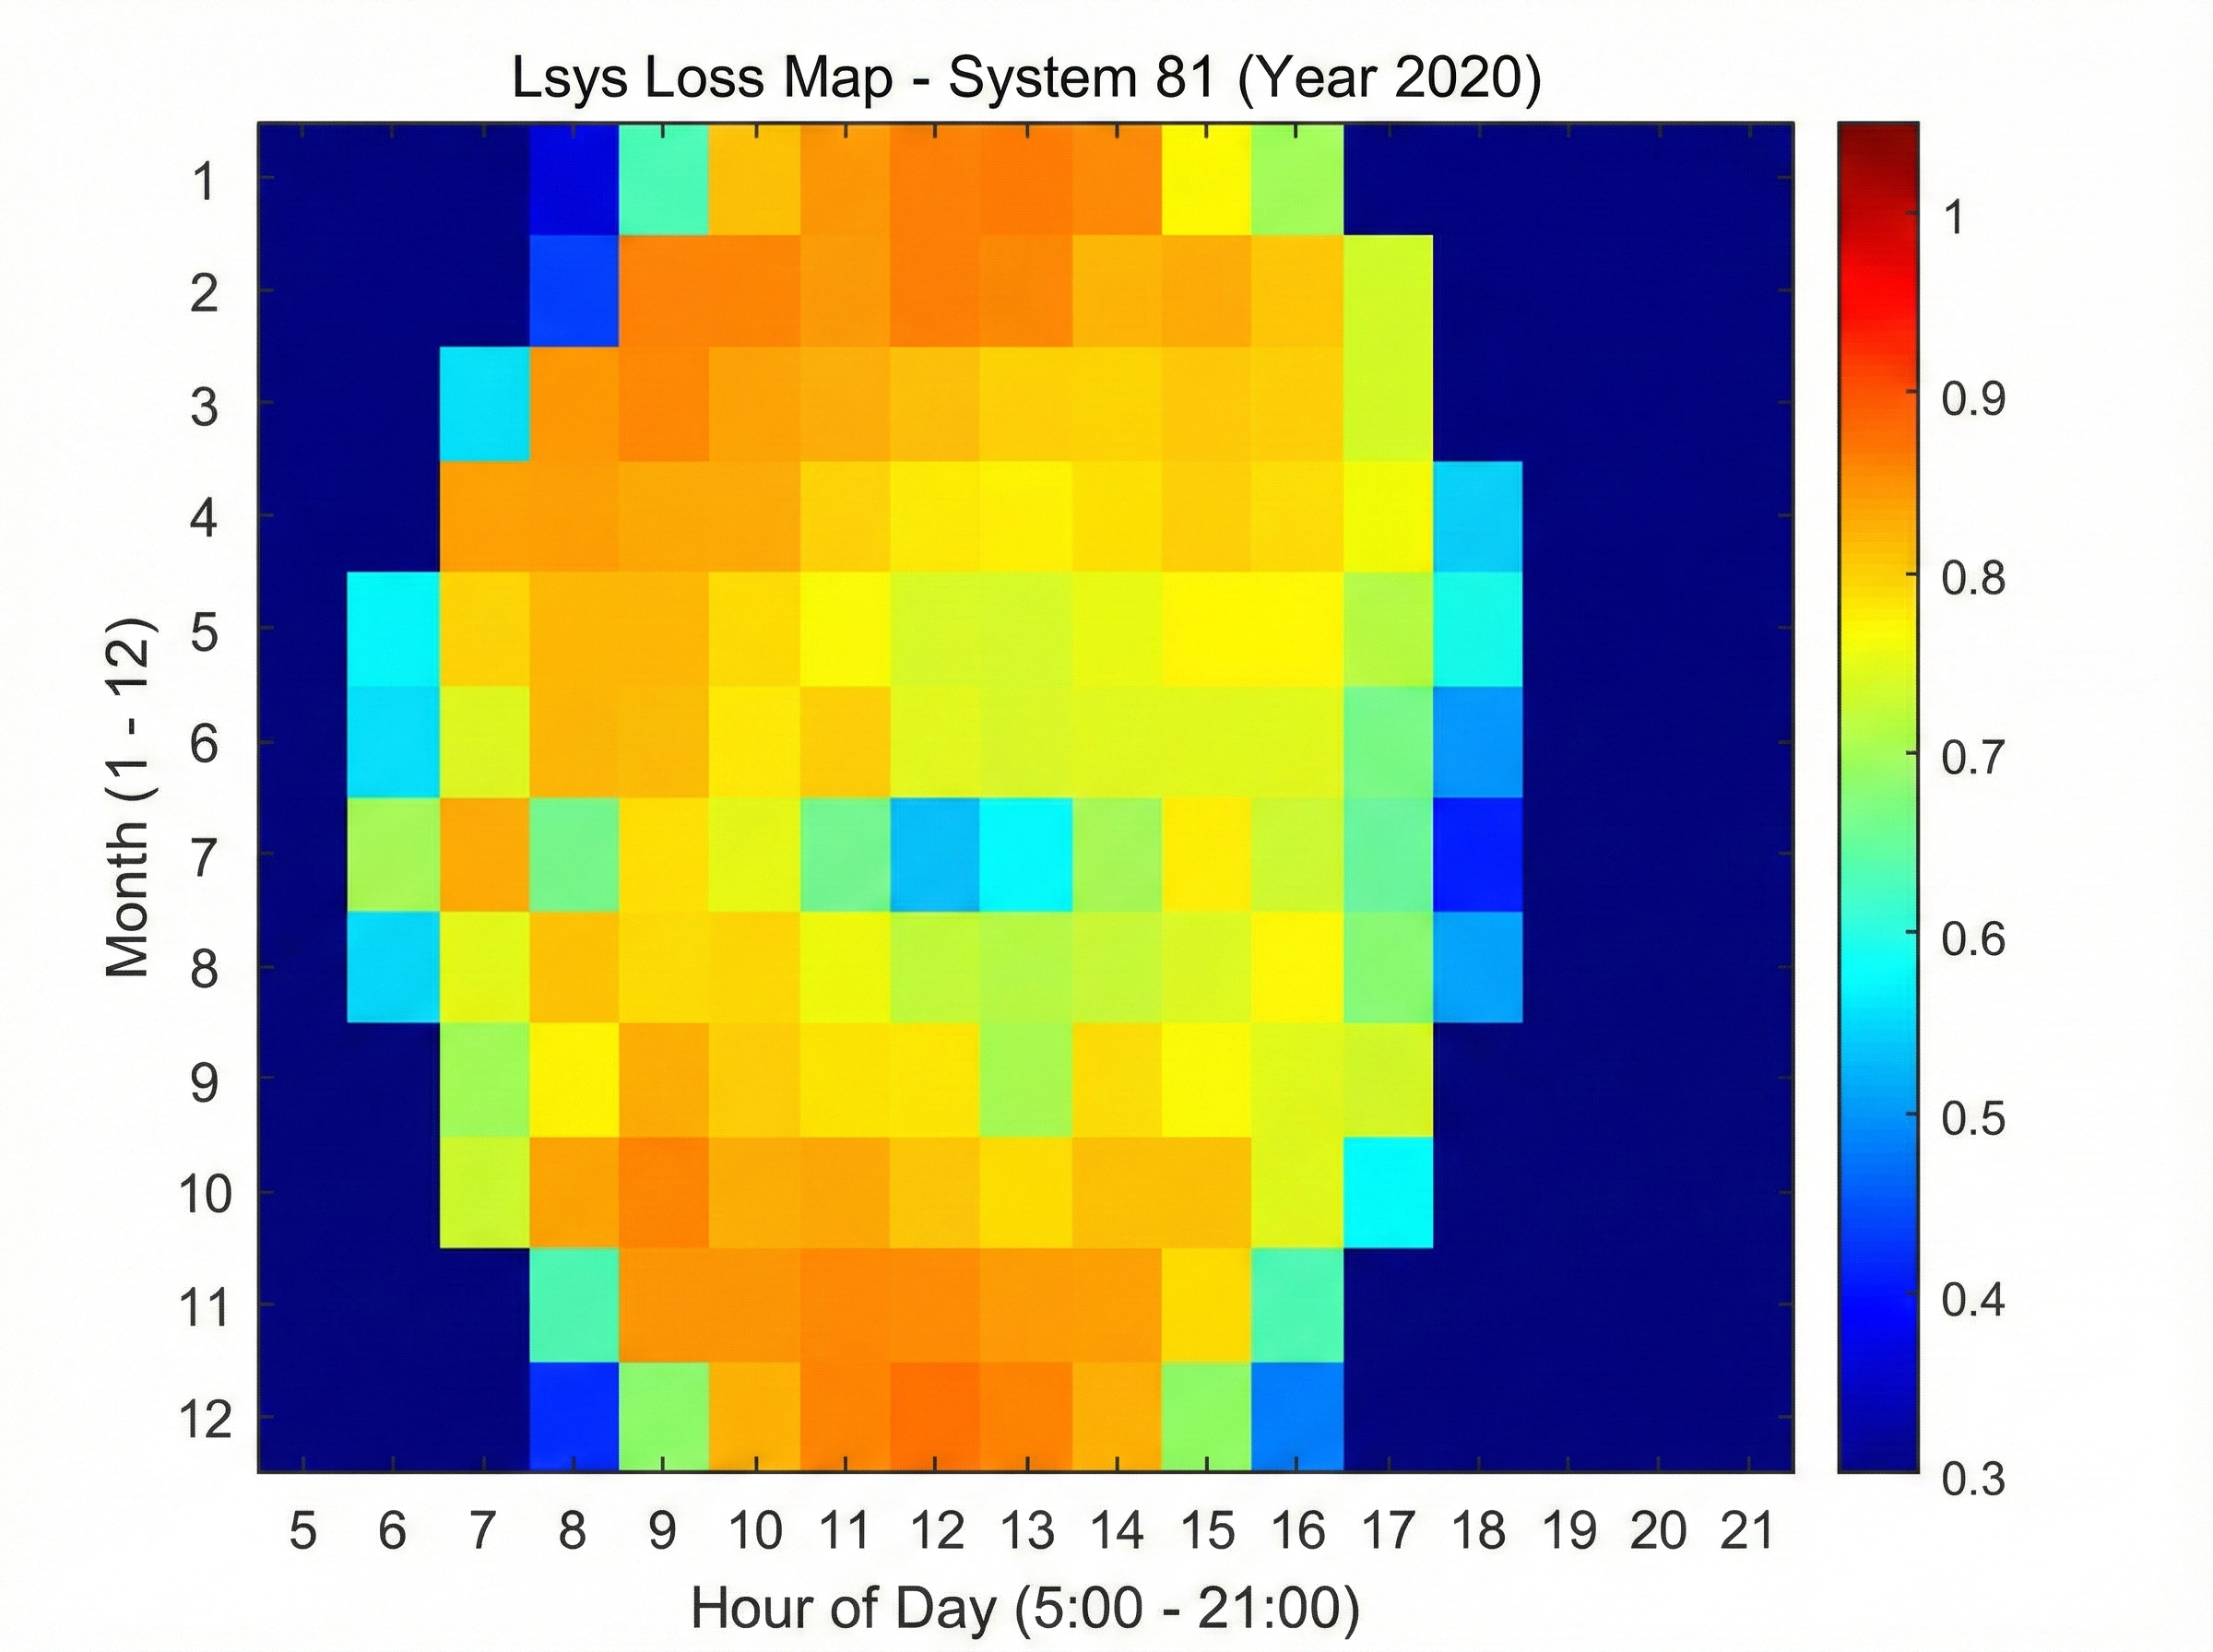
\includegraphics[width=\textwidth]{foto/Ibaraki/Sys81LsysMapWithHighTemperatureLoss.png}
        \caption*{ (a) 損失係数ヒートマップ(夏季の低下) }
    \end{minipage}
    \hfill
    \begin{minipage}[b]{0.48\textwidth}
        \centering
        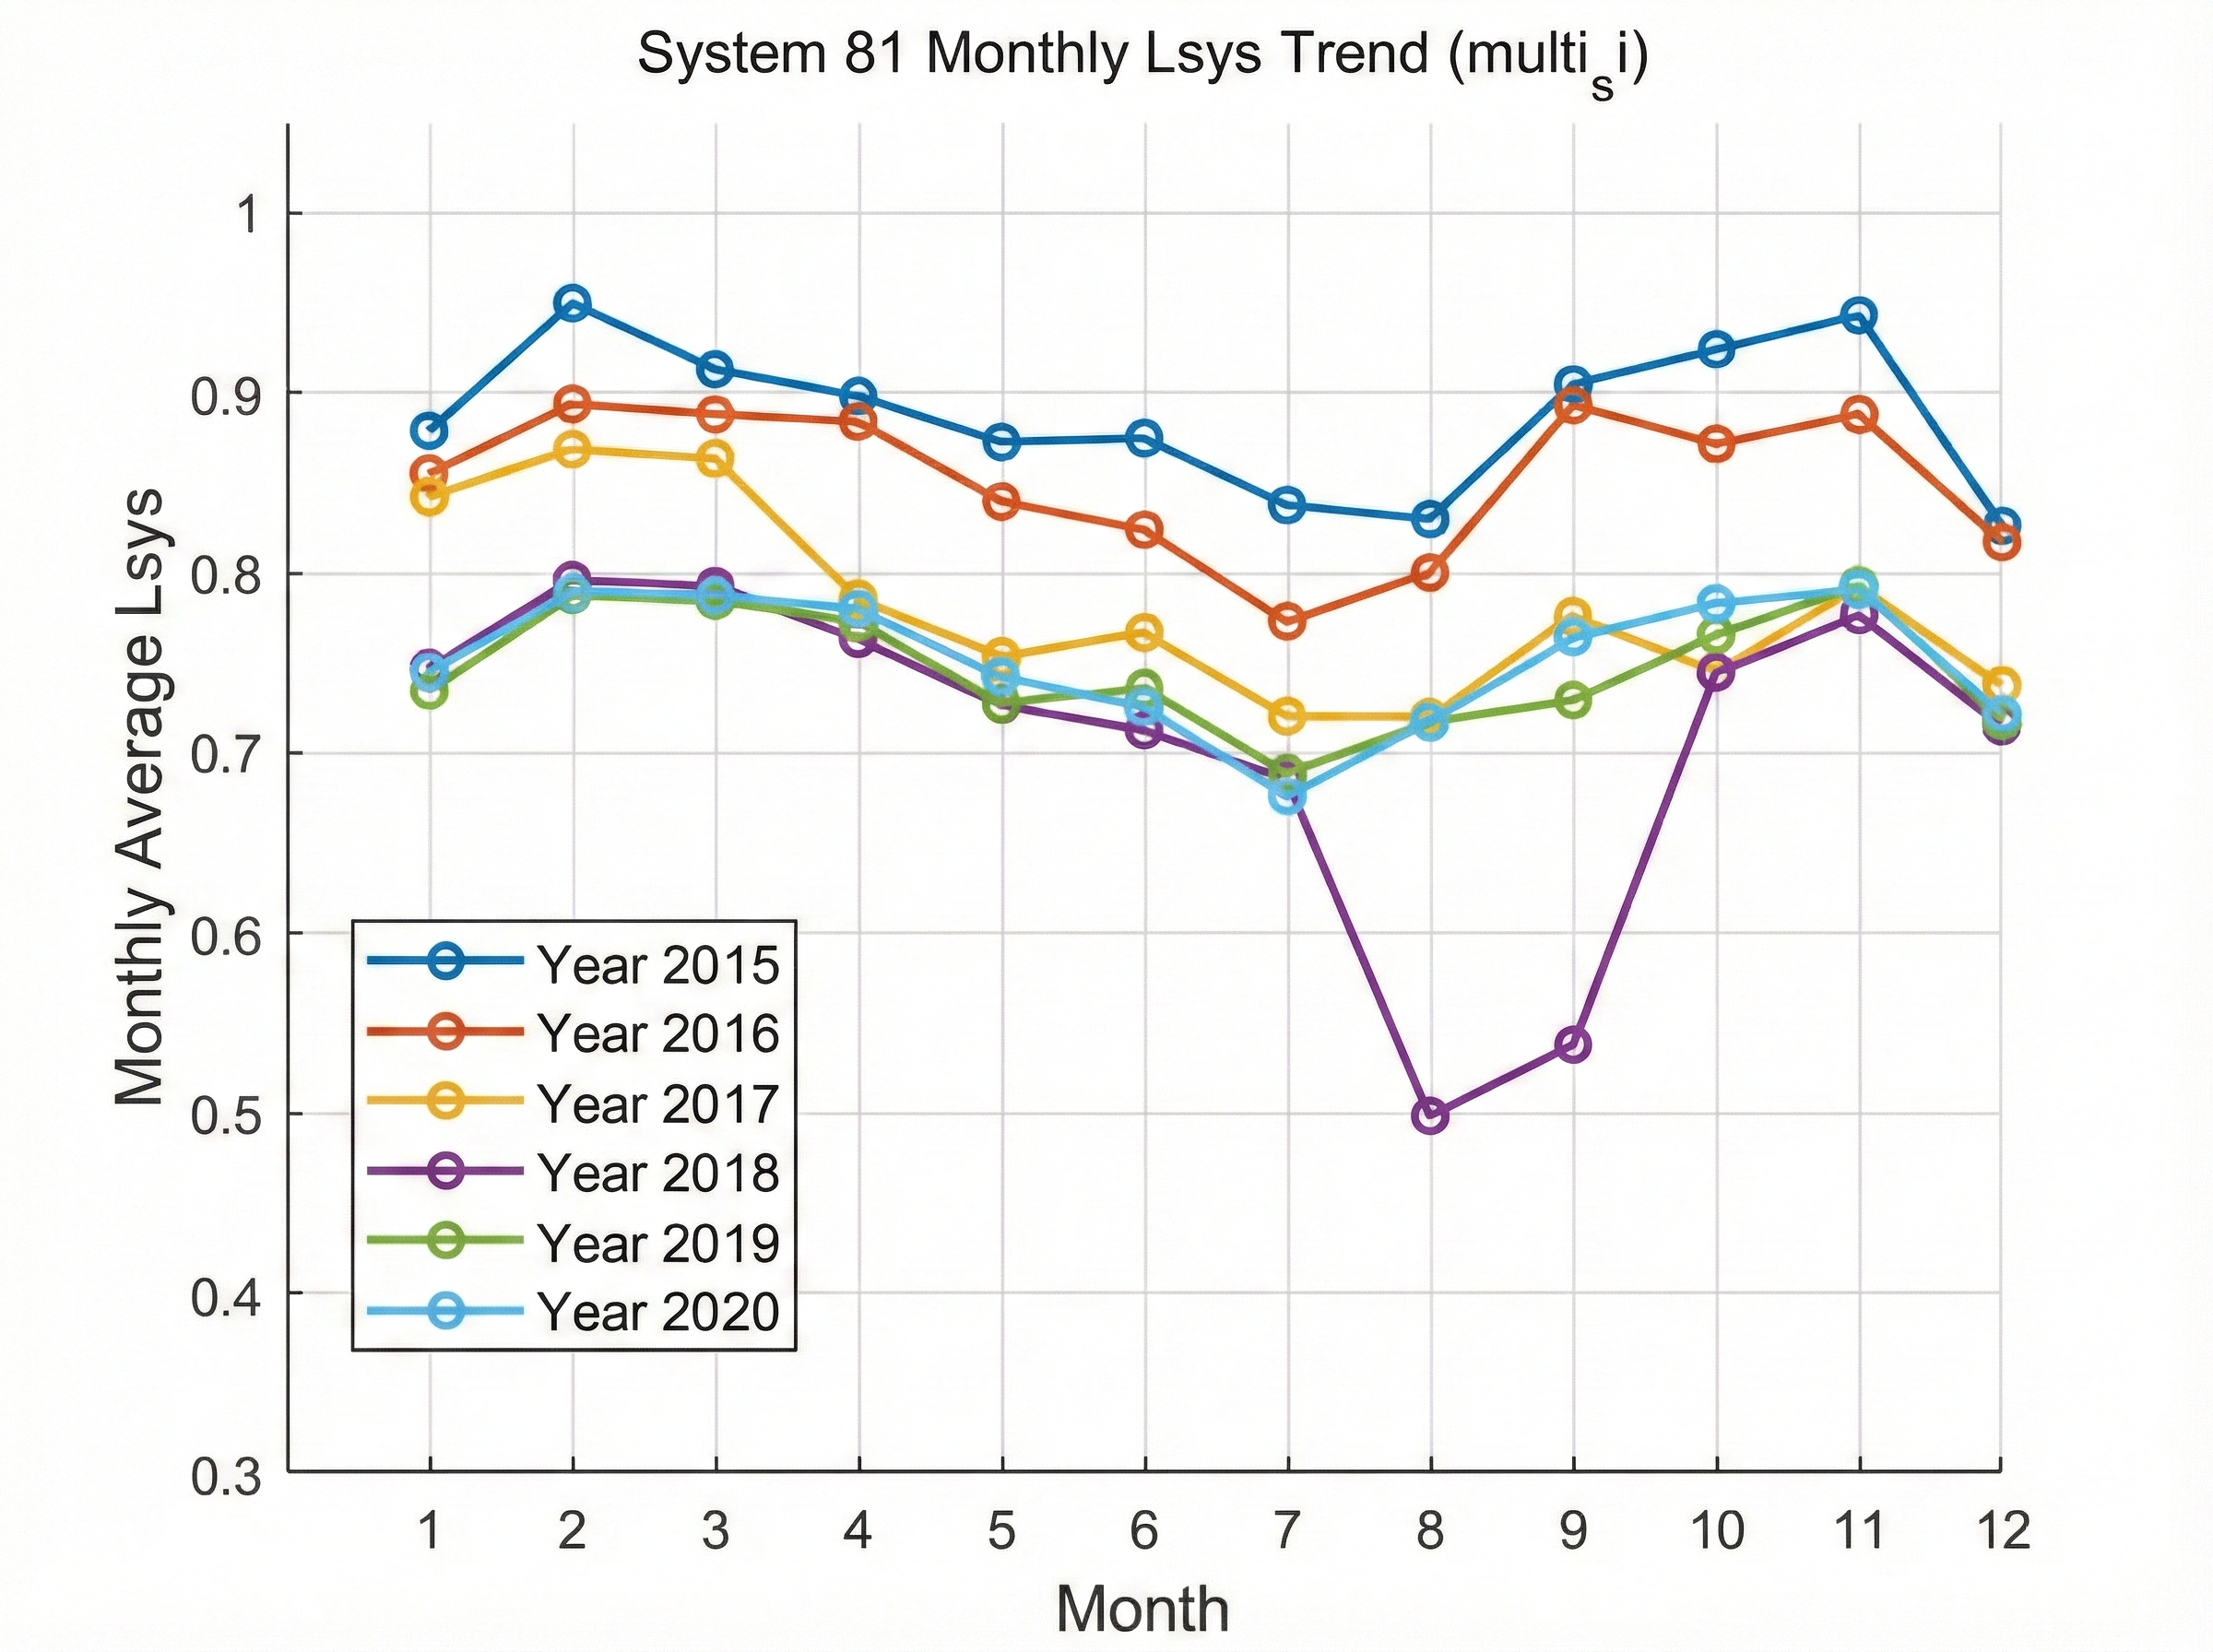
\includegraphics[width=\textwidth]{foto/Ibaraki/Sys81LsysTrendWithHighTemperatureLoss.png}
        \caption*{ (b) 月別経年トレンド}
    \end{minipage}
    \caption{Sys81における損失係数 $L_{sys}$ の季節変動}
    \label{fig:sys81_lsys}
\end{figure}
\FloatBarrier

%------------------------------------------------------------------------
\subsection{衛星推定値および広域観測値との整合性評価}
\label{sec:衛星推定値および広域観測値との整合性評価}
%------------------------------------------------------------------------

本項では、茨城県内に分散するPVシステム群から逆推定された全天日射量($GHI_{est}$)と、参照基準となる広域観測値($GHI_{ref}$)との整合性を評価する。ここで、システム群の中心地での衛星観測データと比較、以下の解析結果は、提案手法がエリア全体の気象トレンドを正確に抽出できていることを示している。

\textbf{推定精度と相関特性の評価}

図\ref{fig:茨城エリアにおける推定日射量と衛星データの相関}に、推定日射量と衛星データの散布図を示す。

グラフを確認すると、データ点は理想線($y=x$)の周囲に広く分布しており、データセットA(北杜市)と比較すると分散は大きい。これは、前述した地理的な距離に起因する不可避な不一致である。しかし、全体的な傾向としては強い線形相関を保っており、低照度から高照度までバイアスの偏りなく分布している。これは、12システムの推定値を統合する過程で、個々の地点における局所的な雲の影響が平滑化され、茨城県エリアとしての平均的な水平面日射量が導出された結果であると解釈できる。

\begin{figure}[htbp]
    \centering
    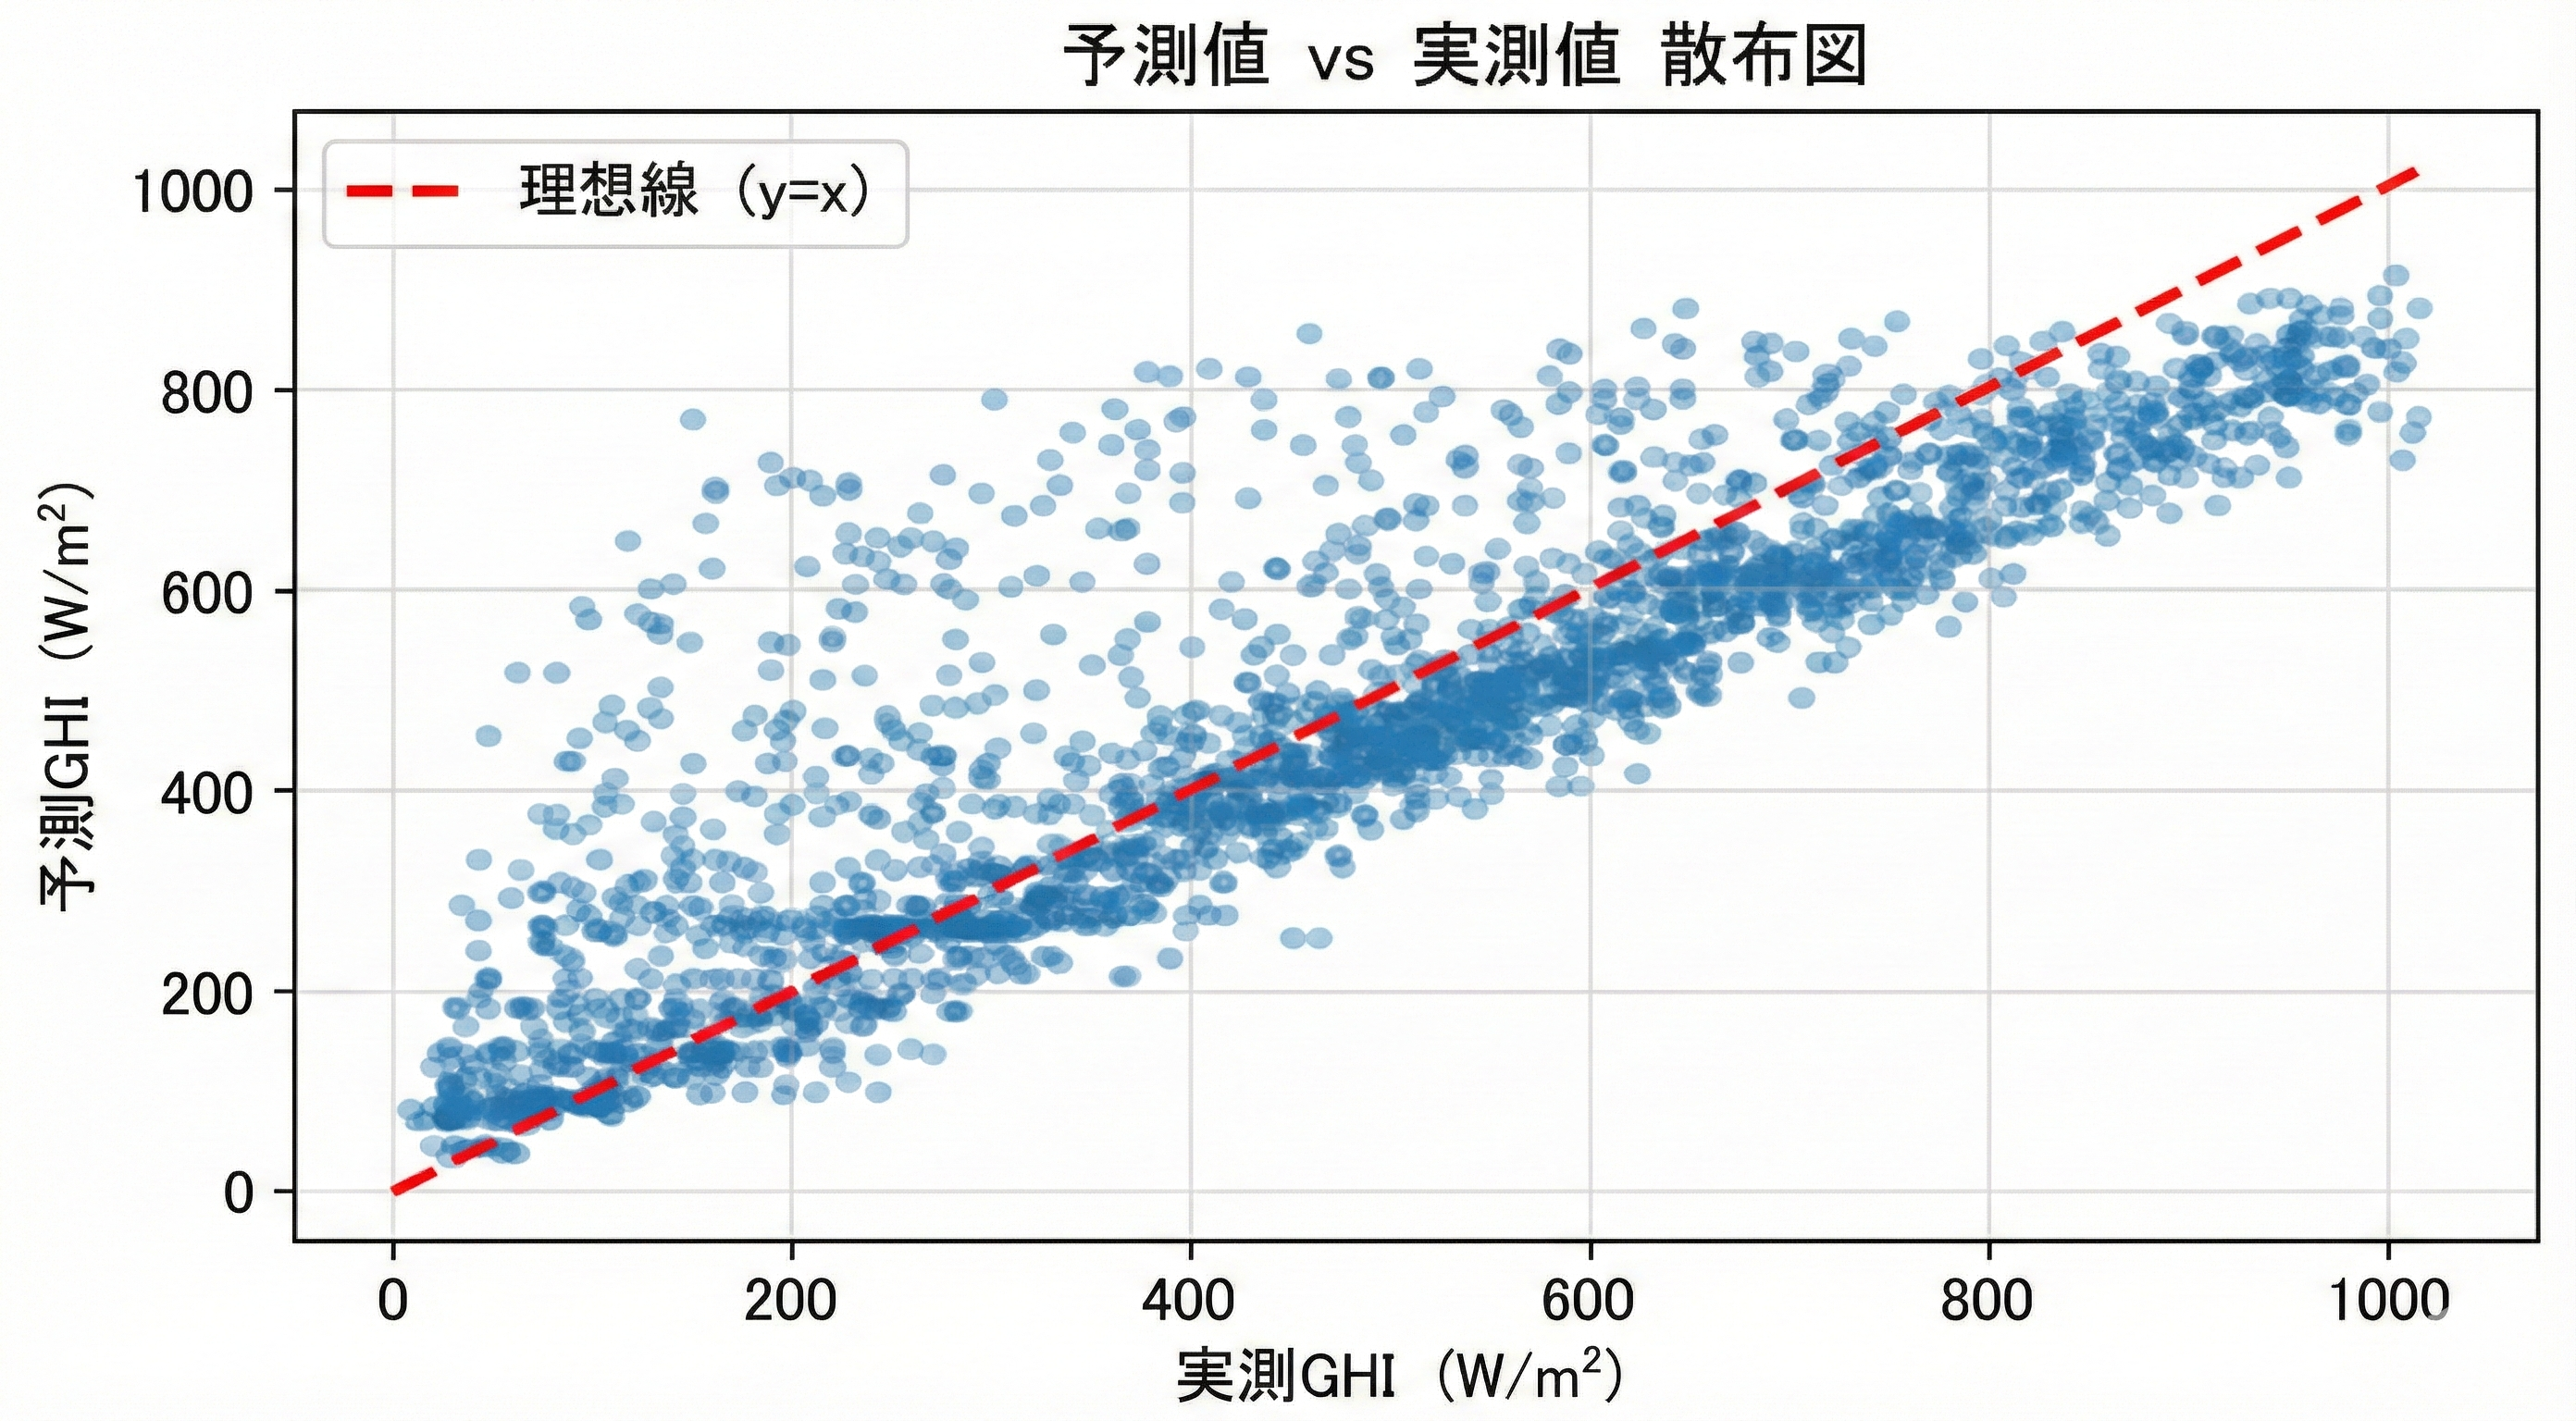
\includegraphics[width=0.8\textwidth]{foto/Ibaraki/ScatterPlot.png}
    \caption{茨城エリアにおける推定日射量と衛星データの相関}
    \label{fig:茨城エリアにおける推定日射量と衛星データの相関}
\end{figure}
\FloatBarrier

\textbf{誤差分布とバイアスの検証}

モデルの物理的な妥当性を検証するため、推定誤差($Error = GHI_{est} - GHI_{ref}$)のヒストグラムを図\ref{fig:広域観測値に対する推定誤差の統計特性}(a)に示す。

解析の結果、平均バイアス誤差(MBE)は \textbf{$-3.6 \mathrm{W/m^2}$} と極めて小さな値となった。参照データが離れた地点のものであるにもかかわらず、バイアスがほぼゼロに収束している事実は重要である。これは、前項で述べた「損失係数 $L_{sys}$ による熱損失等の吸収」が適切に機能し、システムごとの個体差や経年劣化が補正された結果、物理的に正しい日射の絶対値レベルが出力されていることを証明している。

また、図\ref{fig:広域観測値に対する推定誤差の統計特性}(b)の相対誤差分布においても、ピークは0付近にあり、大部分のデータが許容範囲内に収まっている。

\begin{figure}[htbp]
    \centering
    \begin{minipage}[b]{0.48\textwidth}
        \centering
        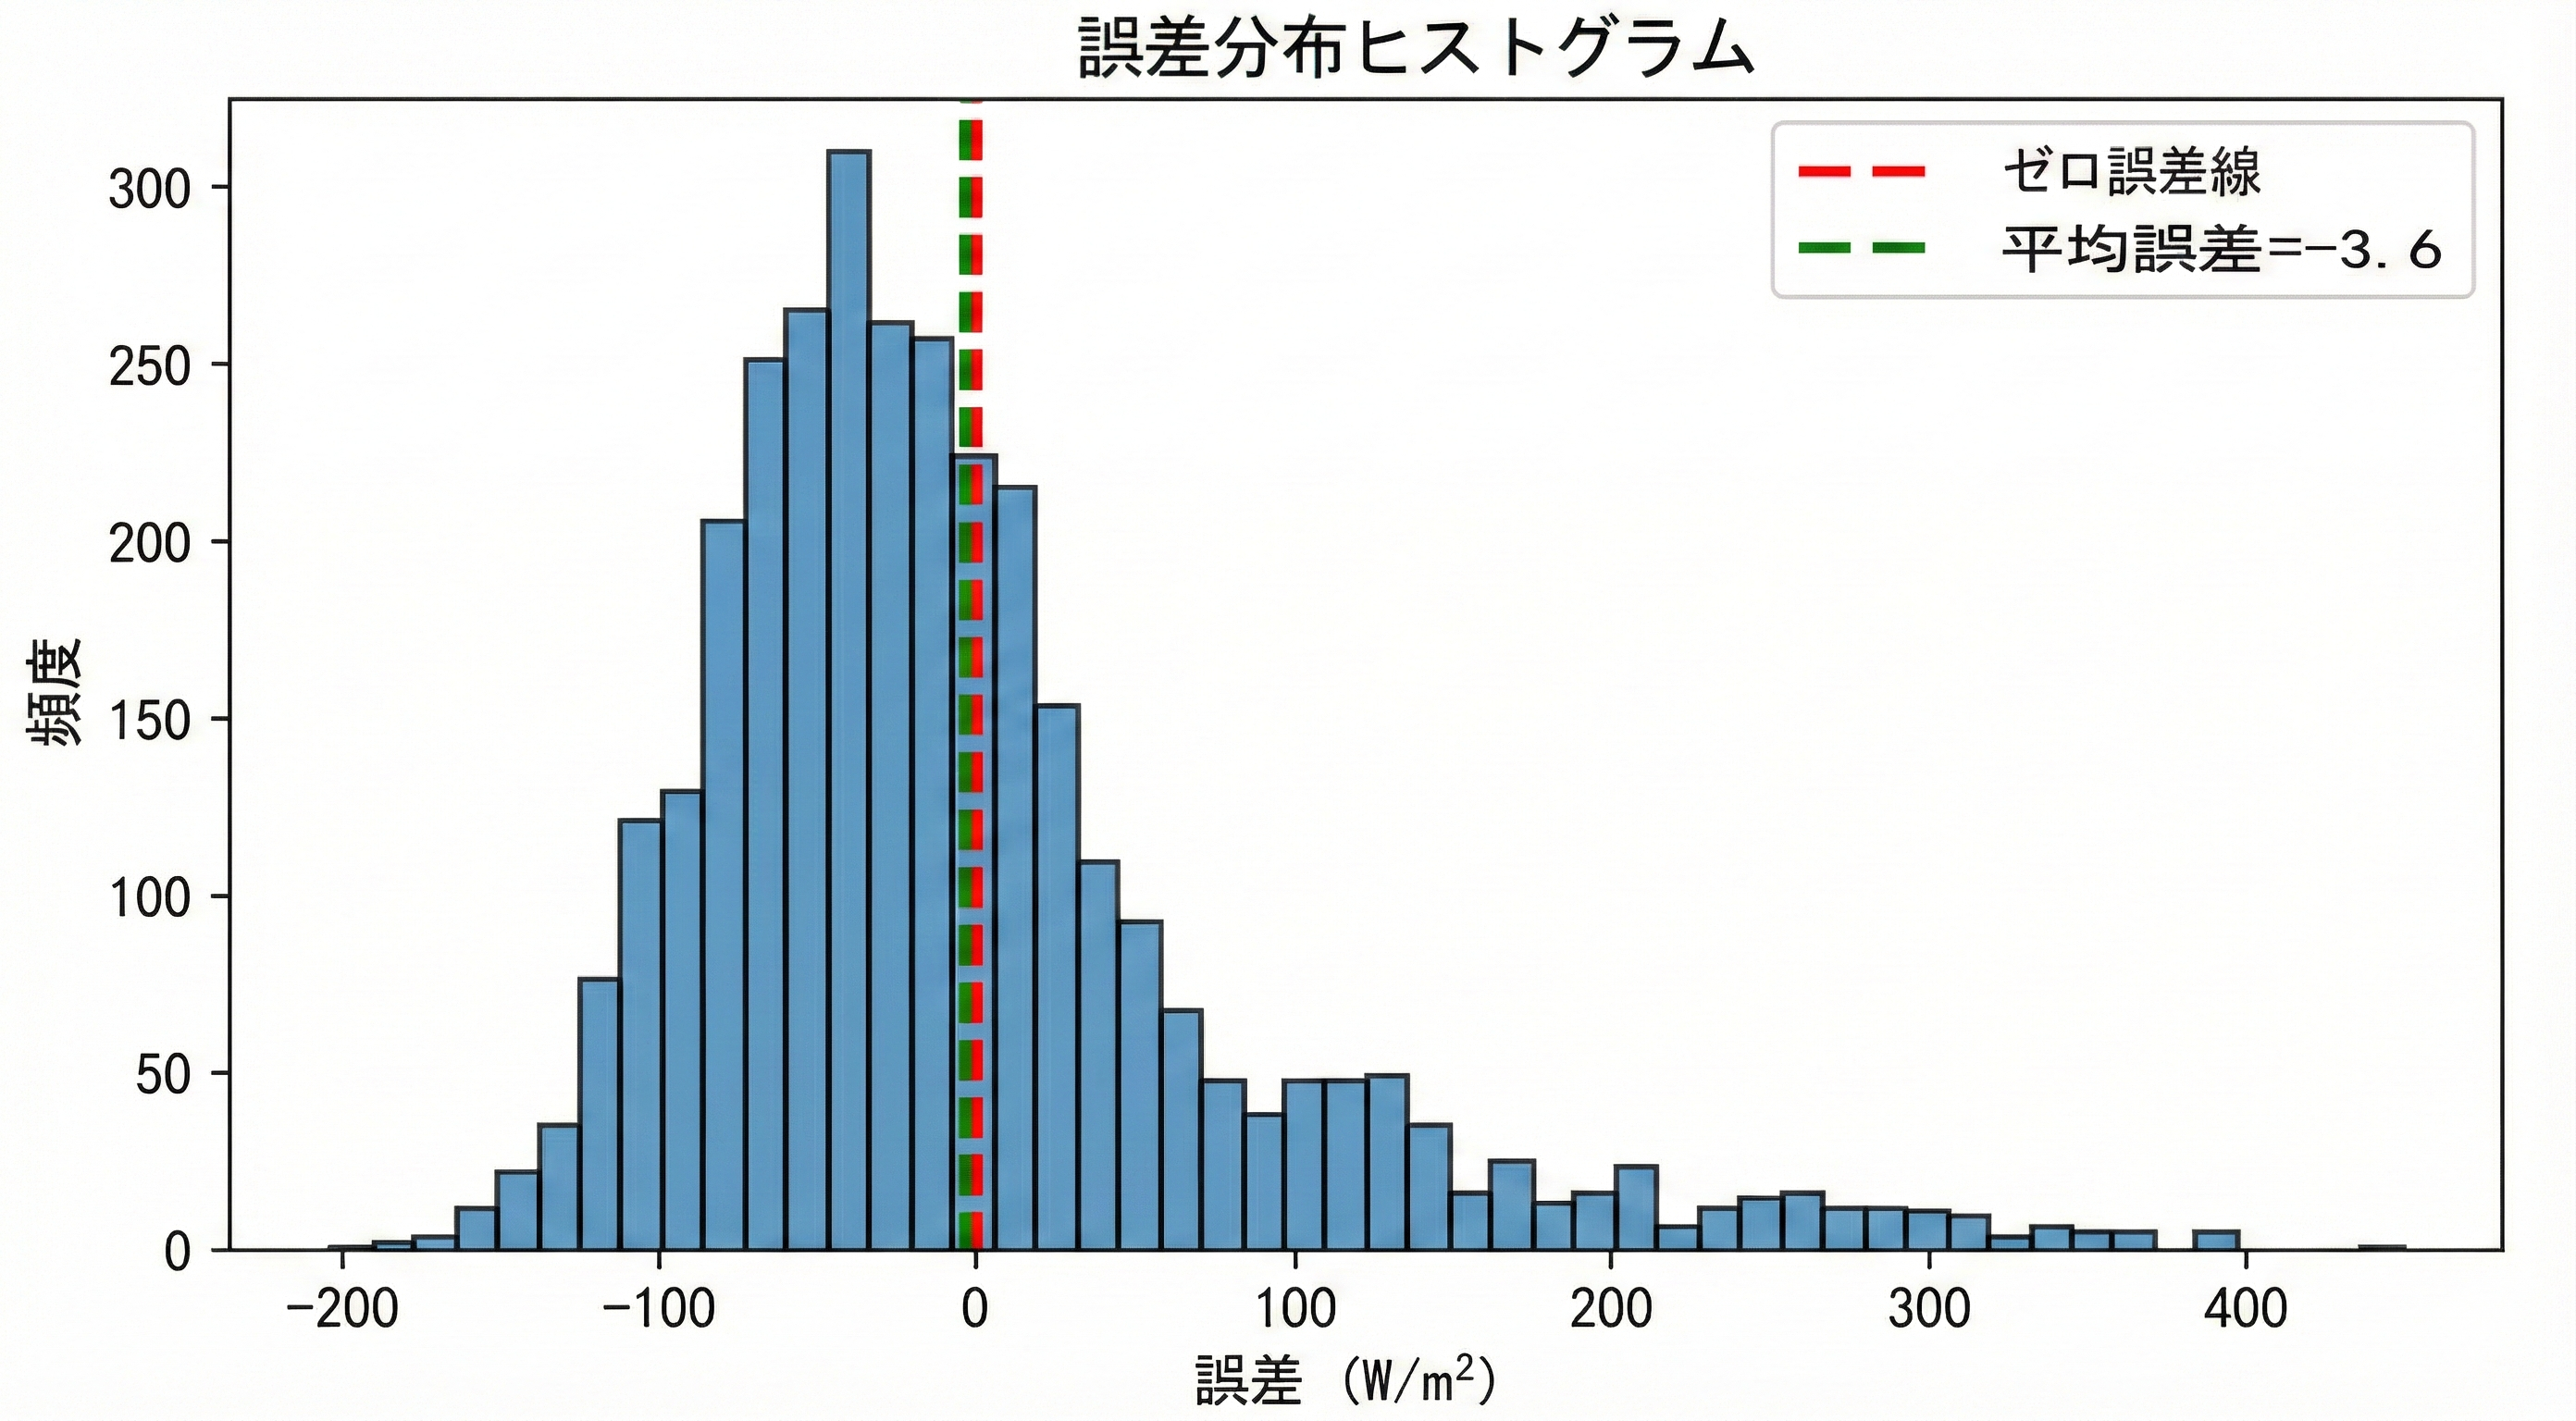
\includegraphics[width=\textwidth]{foto/Ibaraki/ErrorDistribution.png}
        \caption*{ (a) 推定誤差分布 (MBE = -3.6 W/m$^2$) }
    \end{minipage}
    \hfill
    \begin{minipage}[b]{0.48\textwidth}
        \centering
        \includegraphics[width=\textwidth]{foto/Ibaraki/RelativeErrorDistribution.png}
        \caption*{ (b) 相対誤差分布 }
    \end{minipage}
    \caption{広域観測値に対する推定誤差の統計特性}
    \label{fig:広域観測値に対する推定誤差の統計特性}
\end{figure}
\FloatBarrier

\textbf{最終合成カーブの時系列特性}

図\ref{fig:動的選択により再構築された茨城エリアの最適GHIカーブ}に、動的選択アルゴリズムにより合成された最終的なGHI時系列カーブを示す。

分散したシステム群から品質スコアの高いデータをつなぎ合わせることで、センサー欠測や通信エラーによるデータ欠損を相互に補完し、物理的に矛盾のない滑らかな日射量波形が再構築されていることが確認できる。

\begin{figure}[htbp]
    \centering
    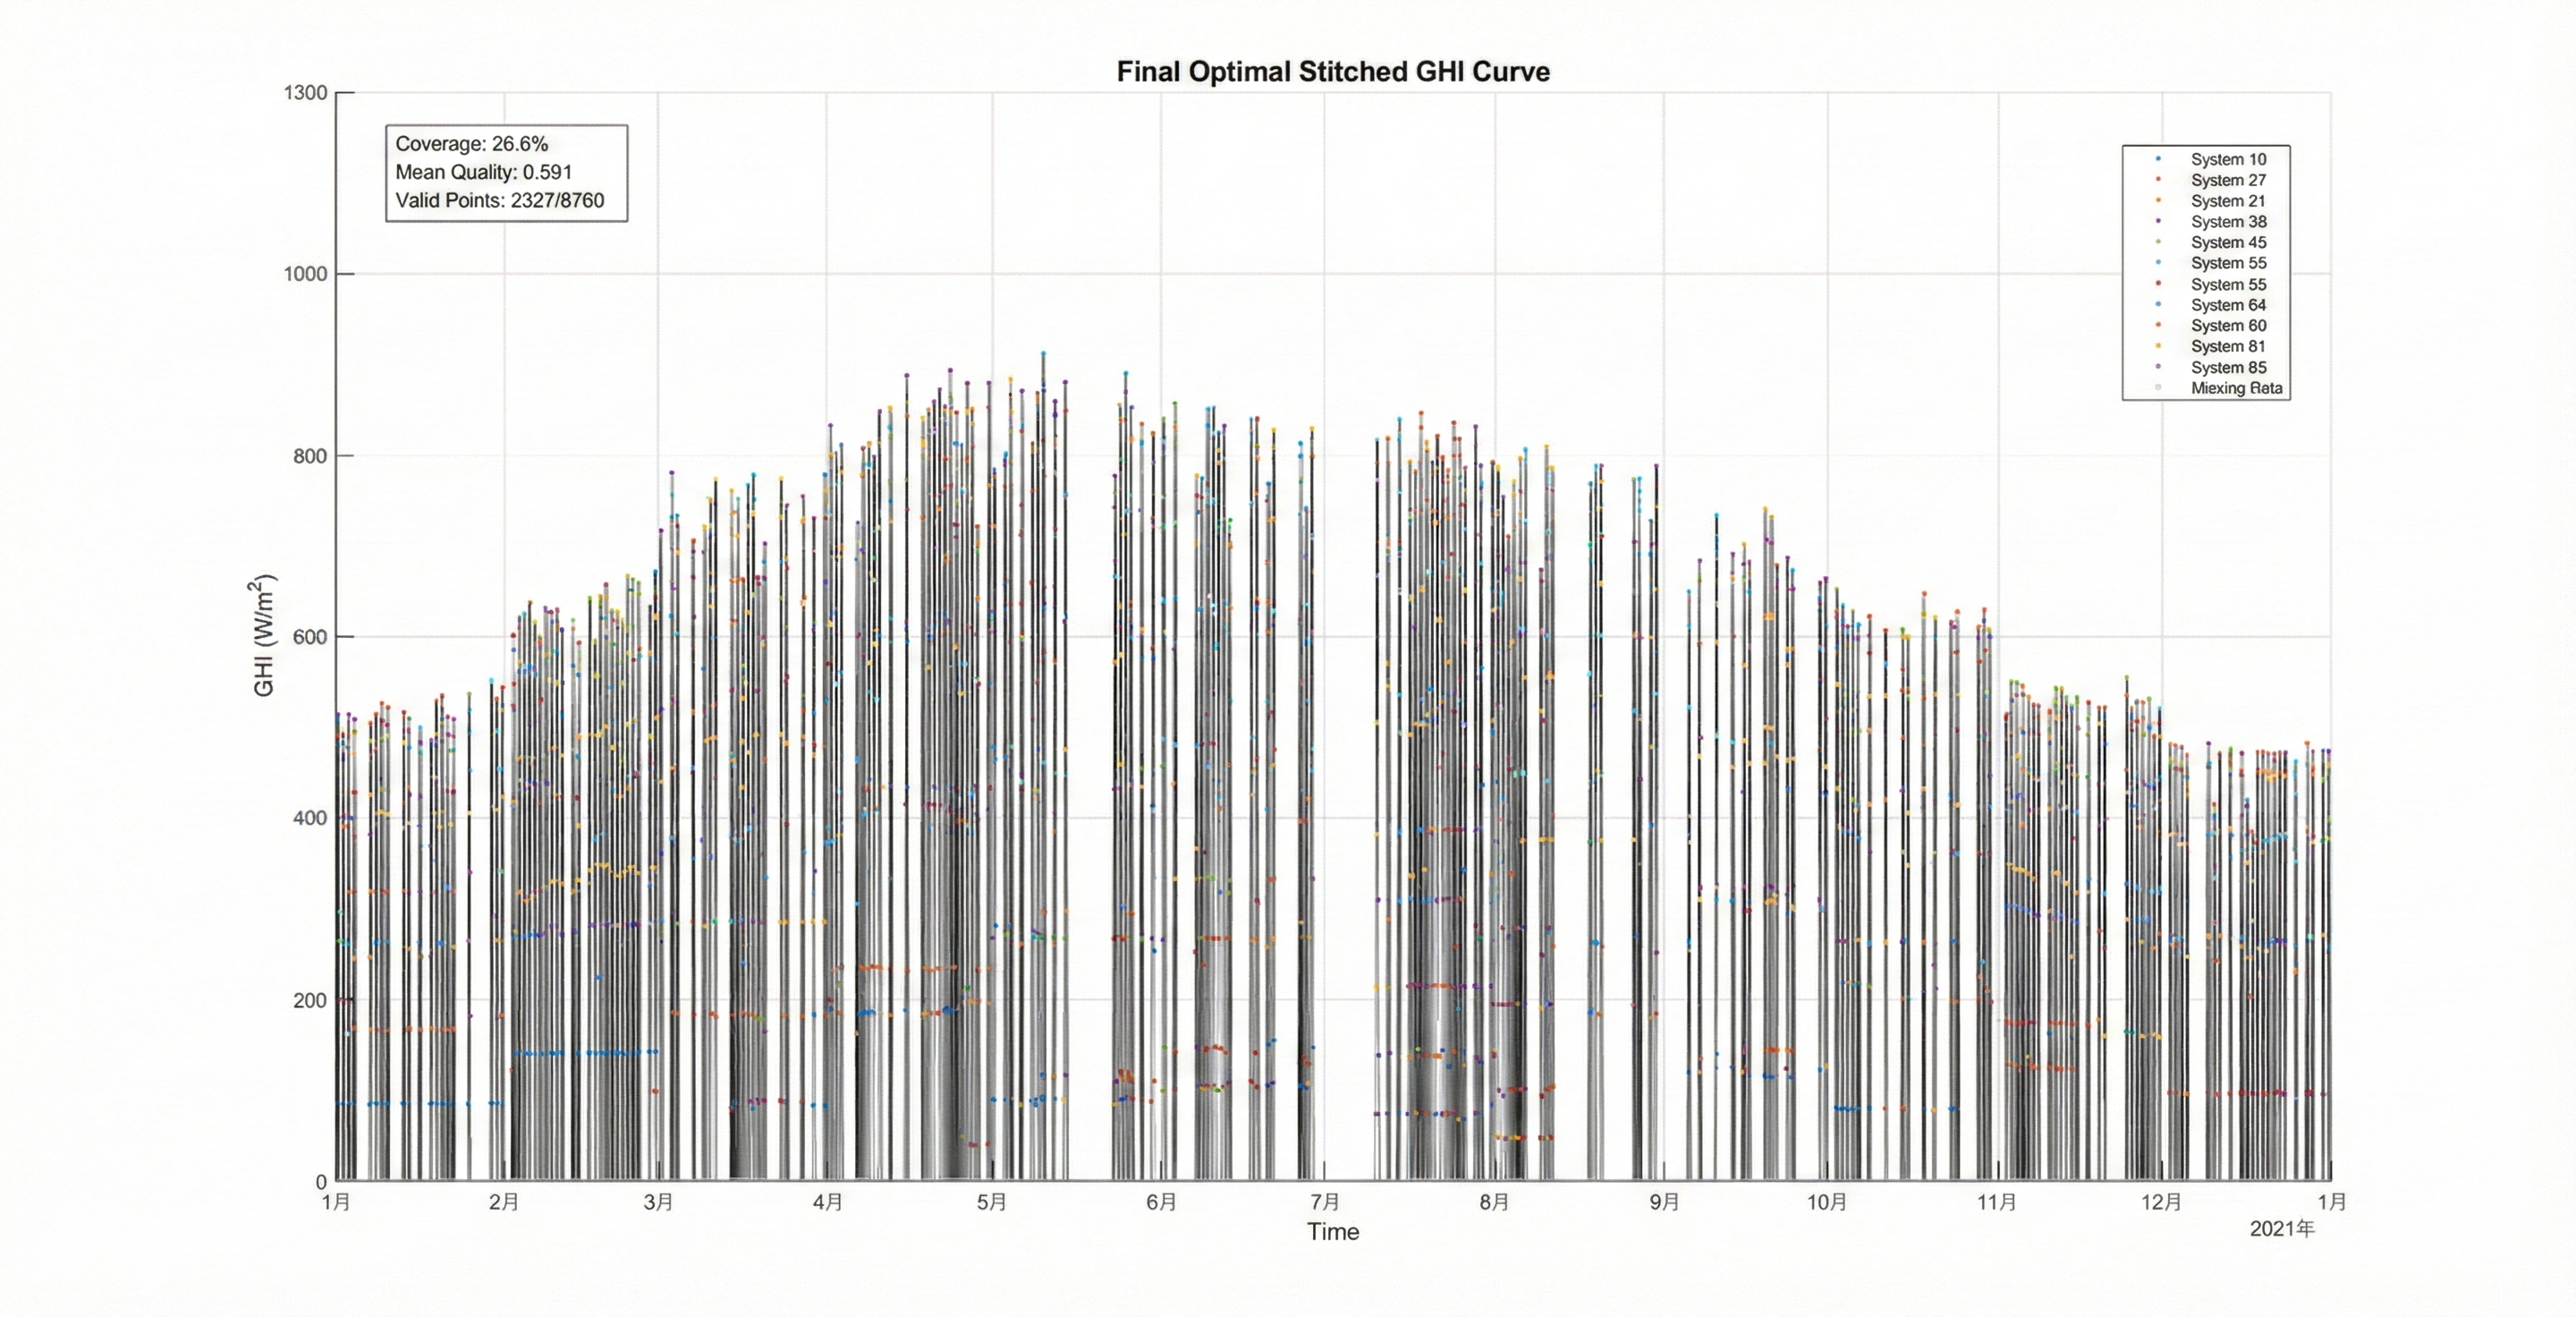
\includegraphics[width=1.0\textwidth]{foto/Ibaraki/FinalGHI.png}
    \caption{動的選択により再構築された茨城エリアの最適GHIカーブ}
    \label{fig:動的選択により再構築された茨城エリアの最適GHIカーブ}
\end{figure}
\FloatBarrier

%------------------------------------------------------------------------
\subsection{地理的分散と気象不一致による誤差特性の分析}
\label{sec:地理的分散誤差分析}
%------------------------------------------------------------------------

前項では全体としての平均的な整合性が確認されたが、詳細な誤差分布を確認すると、地理的な位置の不一致やセンサー情報の不足に起因する、Dataset A(北杜サイト)とは異なる特有のバイアス特性が観察された。

\textbf{日射強度依存性と熱損失の影響}

図\ref{fig:日射強度に依存する推定誤差特性}に、実測GHIに対する残差プロットおよび強度区分別の平均誤差を示す。
Dataset Aと同様に、ここでも日射強度に応じた系統的なバイアス変動が確認されるが、その傾向はより顕著である。

\begin{enumerate}
    \item \textbf{低~中照度域(0-300 W/m$^2$)の正バイアス}: 
    平均 $+20 \sim +30$ W/m$^2$ 程度の過大評価が見られる。これは、衛星観測地点が晴れていても、各PVサイト上空に局所的な雲が存在する場合、あるいは衛星データの空間平均化処理において、薄い雲の影響が十分に反映されなかった場合に生じる「観測視差」の影響と考えられる。
    
    \item \textbf{高照度域(600 W/m$^2$以上)の顕著な負バイアス}: 
    600 W/m$^2$ を超える領域では、平均 $-20 \sim -30$ W/m$^2$ という大きな負のバイアス(過小評価)が発生している。
    この主たる要因は、\textbf{「モジュール温度データの欠落」}である。本データセットでは温度補正項を使用せず、損失係数 $L_{sys}$ に熱損失を吸収させている。しかし、 $L_{sys}$ は月単位の平均的な挙動を示す定数であるため、快晴時の正午付近など、モジュール温度が著しく上昇する(例:50$^\circ$C以上)瞬間的な効率低下を完全には追従できない。その結果、実際の出力低下をモデルが「日射が弱い」と誤認し、推定値を低く算出してしまう現象が表れている。
\end{enumerate}

\begin{figure}[htbp]
    \centering
    \begin{minipage}[b]{0.48\textwidth}
        \centering
        \includegraphics[width=\textwidth]{foto/Ibaraki/ErrorBiosDetect.jpg}
        \caption*{ (a) 系統的バイアス分布 }
    \end{minipage}
    \hfill
    \begin{minipage}[b]{0.48\textwidth}
        \centering
        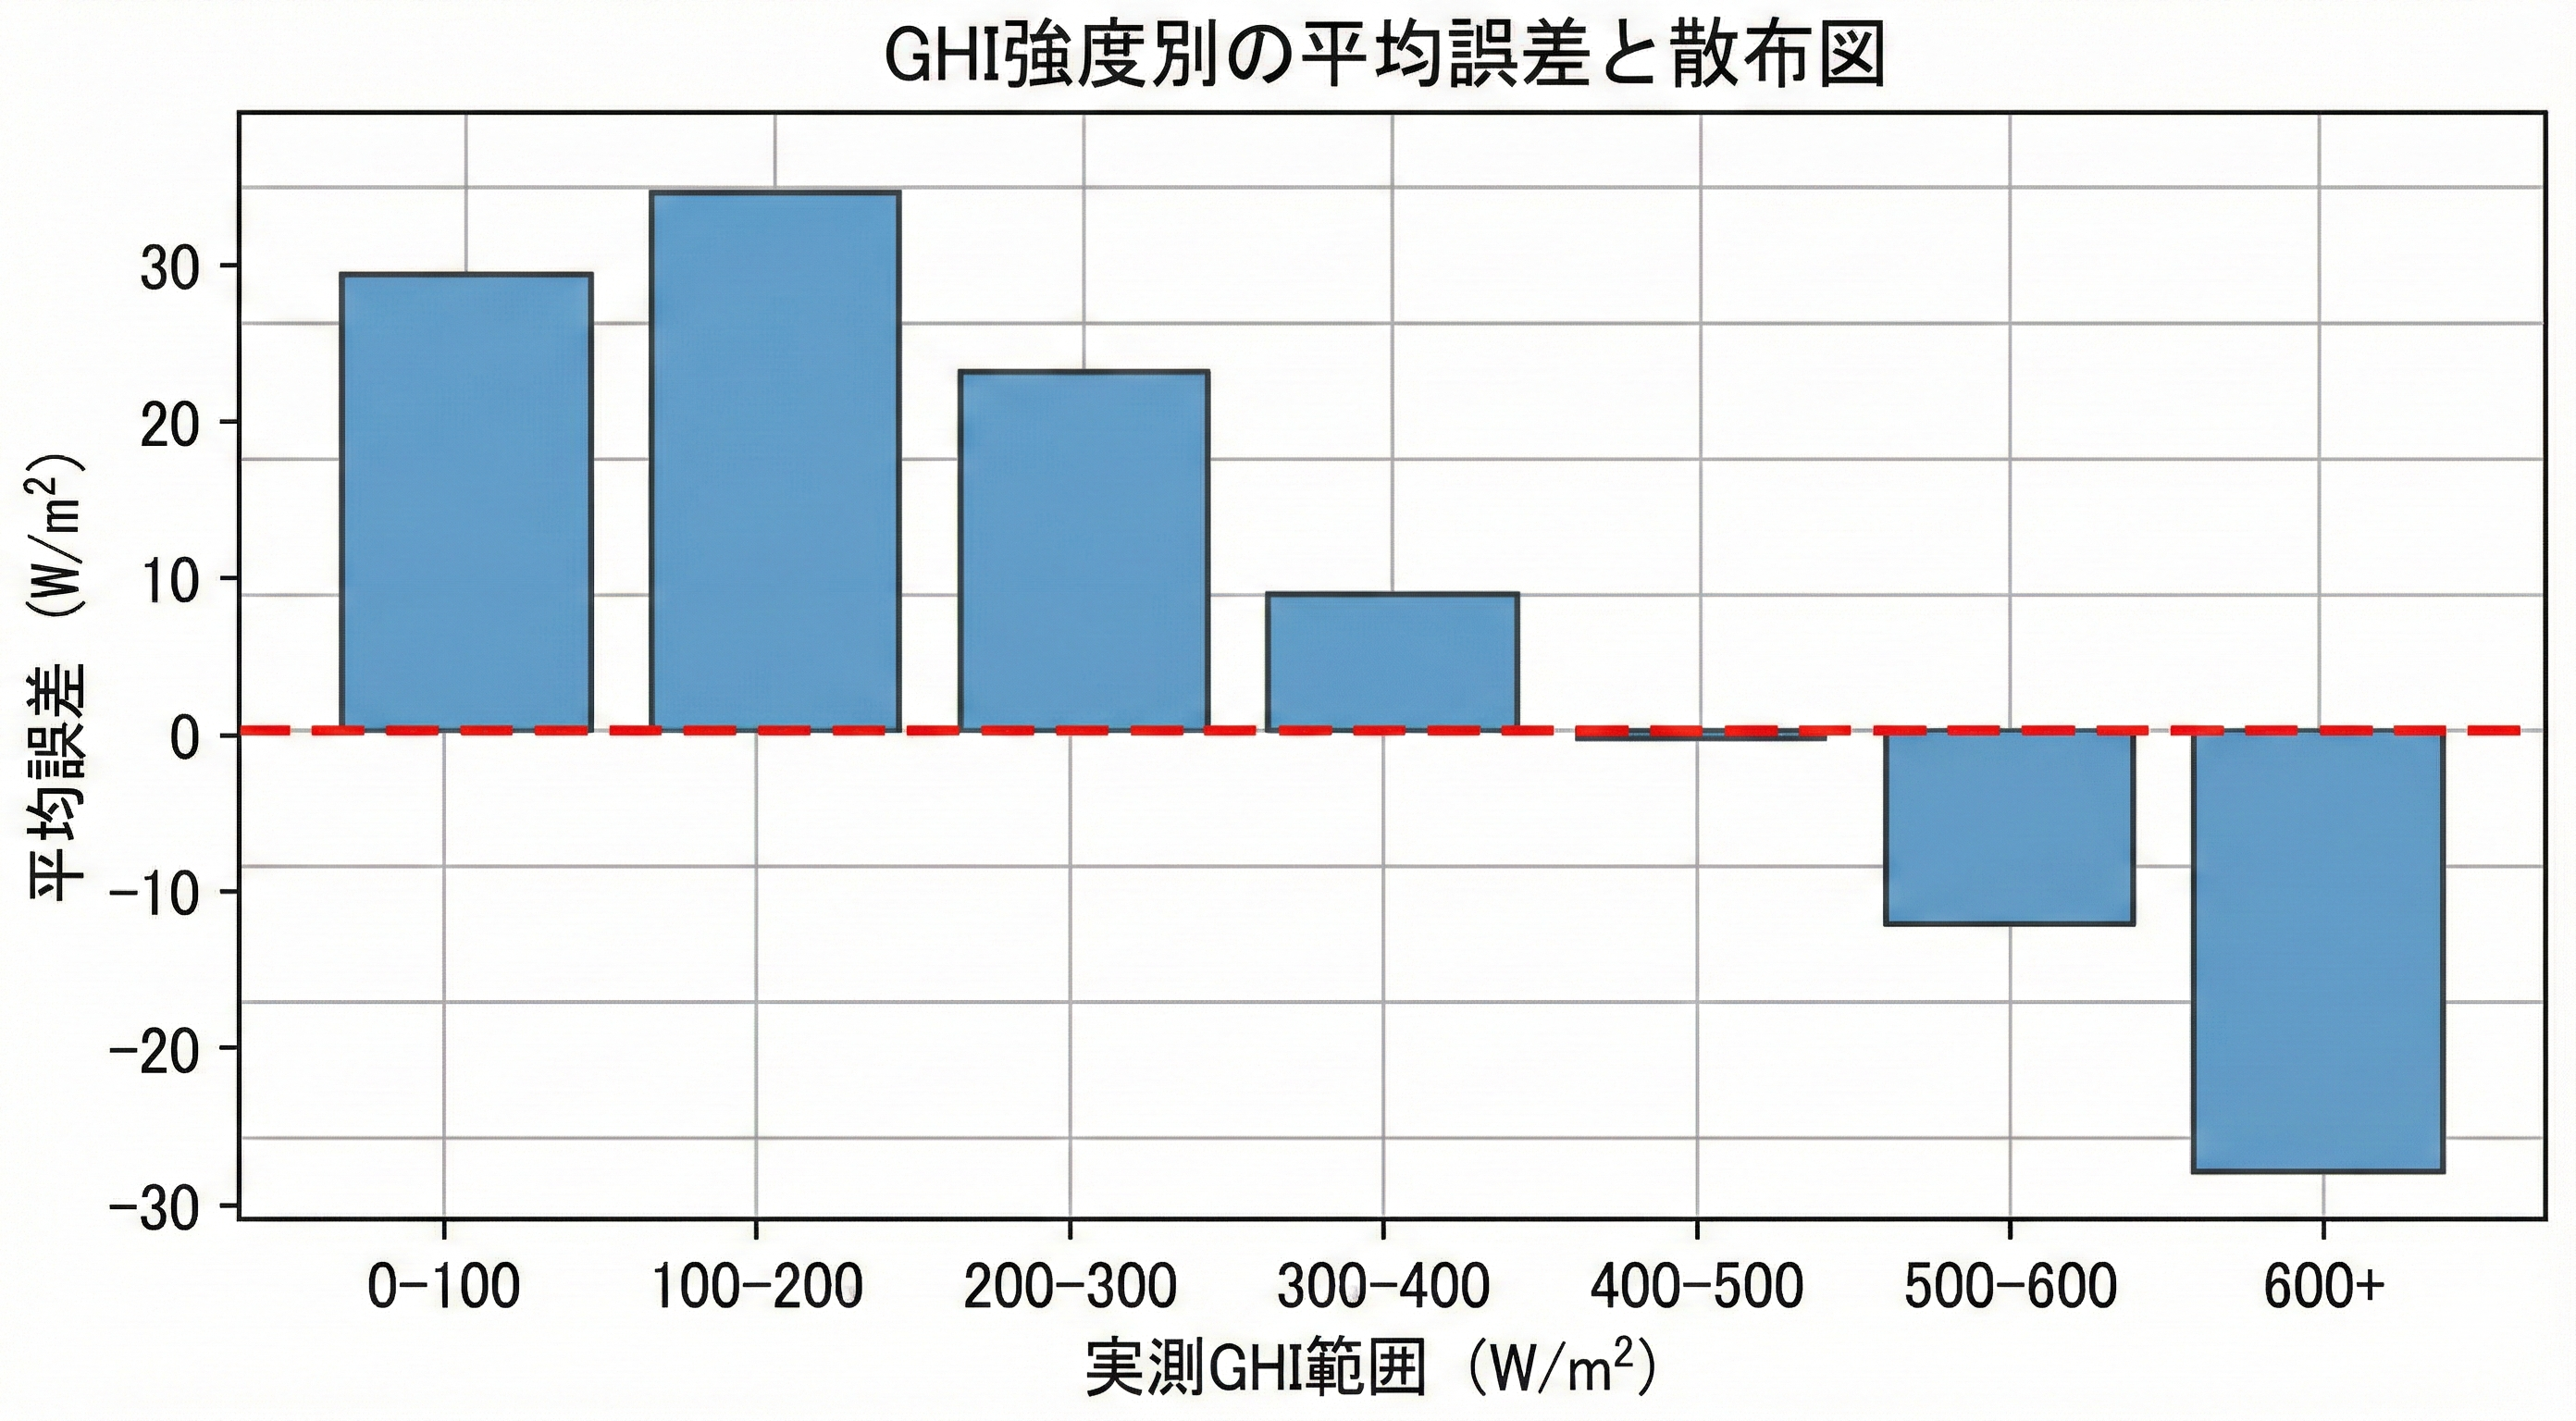
\includegraphics[width=\textwidth]{foto/Ibaraki/AverageErrorInDifferentGHI.png}
        \caption*{ (b) GHI強度別の平均誤差 }
    \end{minipage}
    \caption{日射強度に依存する推定誤差特性}
    \label{fig:日射強度に依存する推定誤差特性}
\end{figure}

\textbf{地理的距離に起因する時間的誤差}

図\ref{fig:時間的および季節的な誤差変動特性}(a)に、時刻別の誤差分布(箱ひげ図)を示す。

正午付近(11時~13時)において、四分位範囲(IQR)および外れ値の幅が最大となっている。Dataset Aと比較してこの分散が極めて大きい理由は、PVシステム設置点と衛星観測点との地理的な距離(数km~数十km)にある。そして正午は放射が最も強くなる時間帯であり、温度損失が増大することに発生する。

\textbf{季節変動と衛星推定特有のバイアス}

図\ref{fig:時間的および季節的な誤差変動特性}(b)の月別平均誤差を確認すると、6月に大きな正のバイアス(約 $+60$ W/m$^2$)、10月に大きな負のバイアス(約 $-55$ W/m$^2$)という特異な挙動が見られる。
\begin{itemize}
    \item \textbf{6月(梅雨時期)の過大評価}: 衛星による日射量推定は、雲頂の反射率(アルベド)から地表面日射量を算出するため、梅雨時期のような多層雲や複雑なエアロゾル条件下では、地上実測値(GHI)よりも高い値を推定する傾向があることが知られている。
    \item \textbf{10月の過小評価}: 太陽高度が下がり始める秋季において、分散した各サイト周辺の建物や樹木による影の影響(Dataset Aで検証済み)が顕在化し始めた可能性がある。温度データがないため、この出力低下が日射量低下として直接的に逆推定された結果と考えられる。
\end{itemize}

\begin{figure}[htbp]
    \centering
    \begin{minipage}[b]{0.48\textwidth}
        \centering
        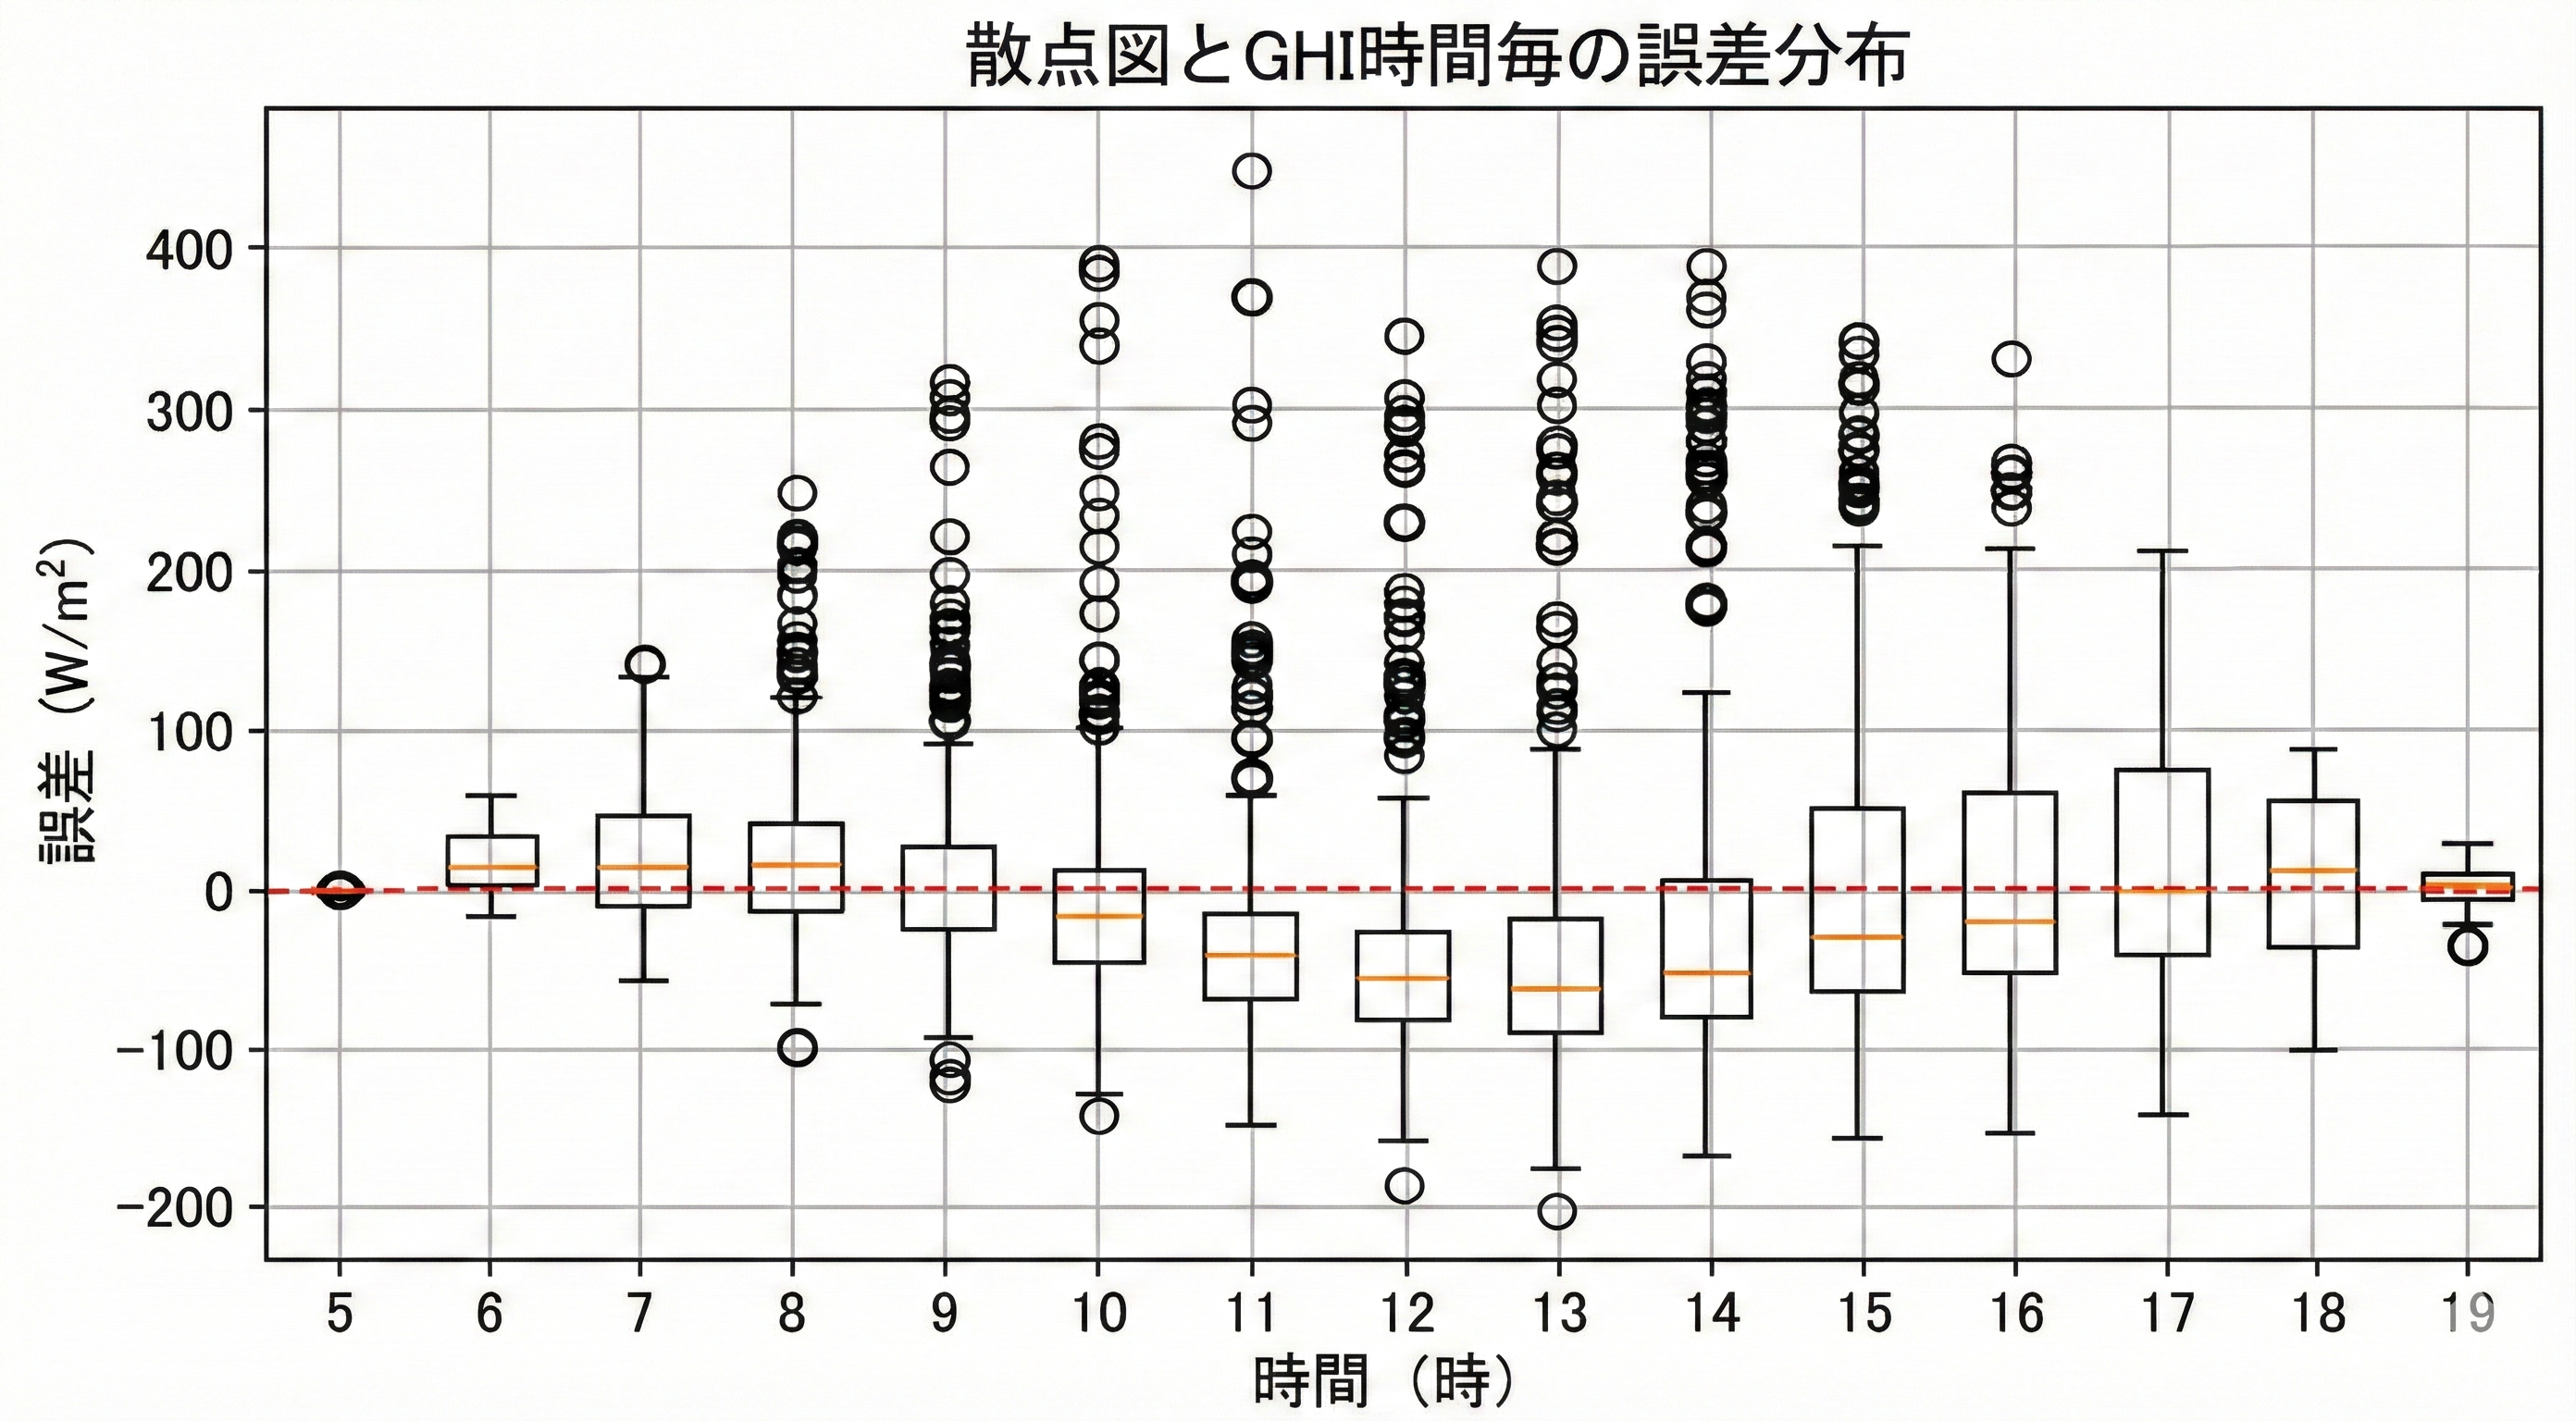
\includegraphics[width=\textwidth]{foto/Ibaraki/GHIErrorDistributionPerHour.png}
        \caption*{ (a) 時刻別誤差分布(距離による分散) }
    \end{minipage}
    \hfill
    \begin{minipage}[b]{0.48\textwidth}
        \centering
        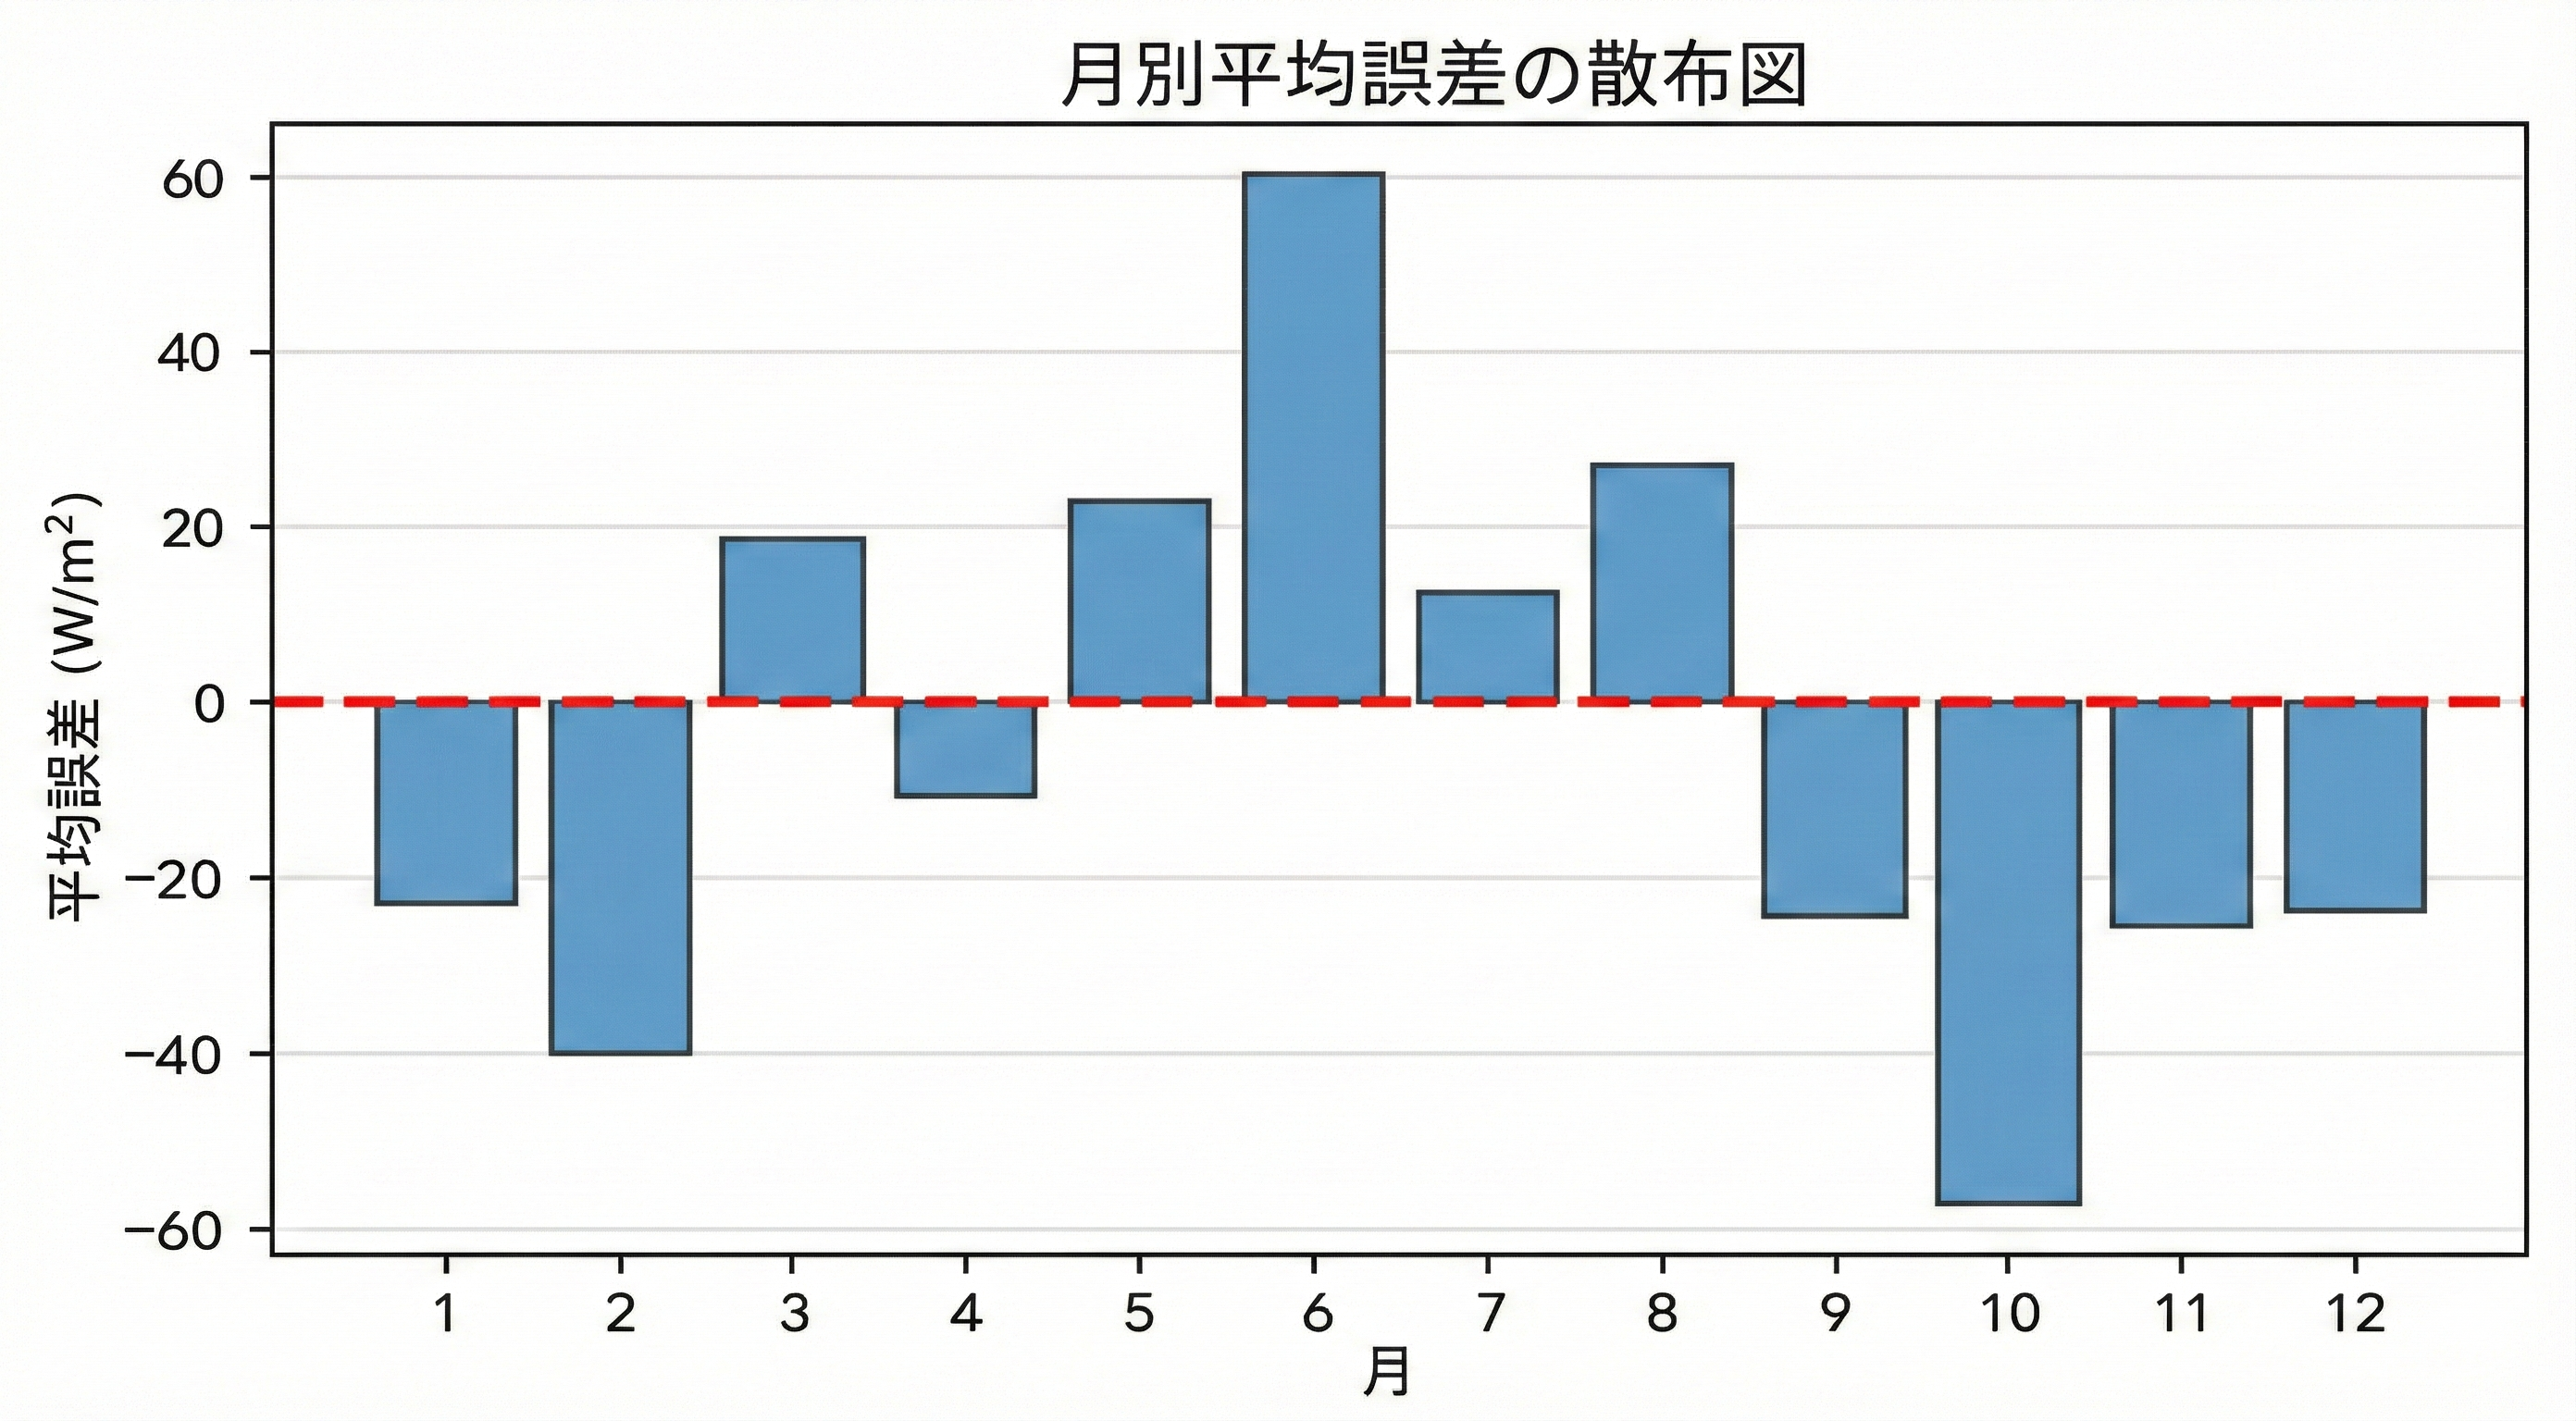
\includegraphics[width=\textwidth]{foto/Ibaraki/MonthErrorDistributionScatterPlot.png}
        \caption*{ (b) 月別平均誤差(季節特有の変動) }
    \end{minipage}
    \caption{時間的および季節的な誤差変動特性}
    \label{fig:時間的および季節的な誤差変動特性}
\end{figure}

%------------------------------------------------------------------------
\subsection{複数システム統合によるロバスト性の検証}
\label{sec:ロバスト性検証}
%------------------------------------------------------------------------

本節の最後に、地理的に分散した複数のPVシステムを統合的に扱うことによる、推定精度の安定化(ロバスト性)効果について検証する。

\textbf{動的選択による最適推定値の合成}

図\ref{fig:分散環境下における各システムの最終GHIカーブへの貢献度}に、最終的なGHIカーブを生成する際に、各システム(System ID 10 $\sim$ 85)の推定値が採用された回数(貢献度)を示す。

グラフからは、特定のシステム(例:Sys 31, 55, 64)が高い頻度で採用されている一方で、他のシステム(例:Sys 66, 81)の寄与は限定的であることが読み取れる。これは、各システムが設置環境(方位・影)や瞬時的な雲の状況によって「品質スコア」を変動させ、アルゴリズムがその時々で最も信頼性の高い(物理モデルとの乖離が小さい)ソースを自律的に選択し続けている結果である。

単一のシステムに依存せず、また単純な平均処理も行わず、地理的に分散した「ポートフォリオ」の中から最良の値を動的に抽出するこの戦略こそが、センサーレスかつ分散環境下においても破綻のない連続的な日射推定を可能にしている要因である。

\begin{figure}[htbp]
    \centering
    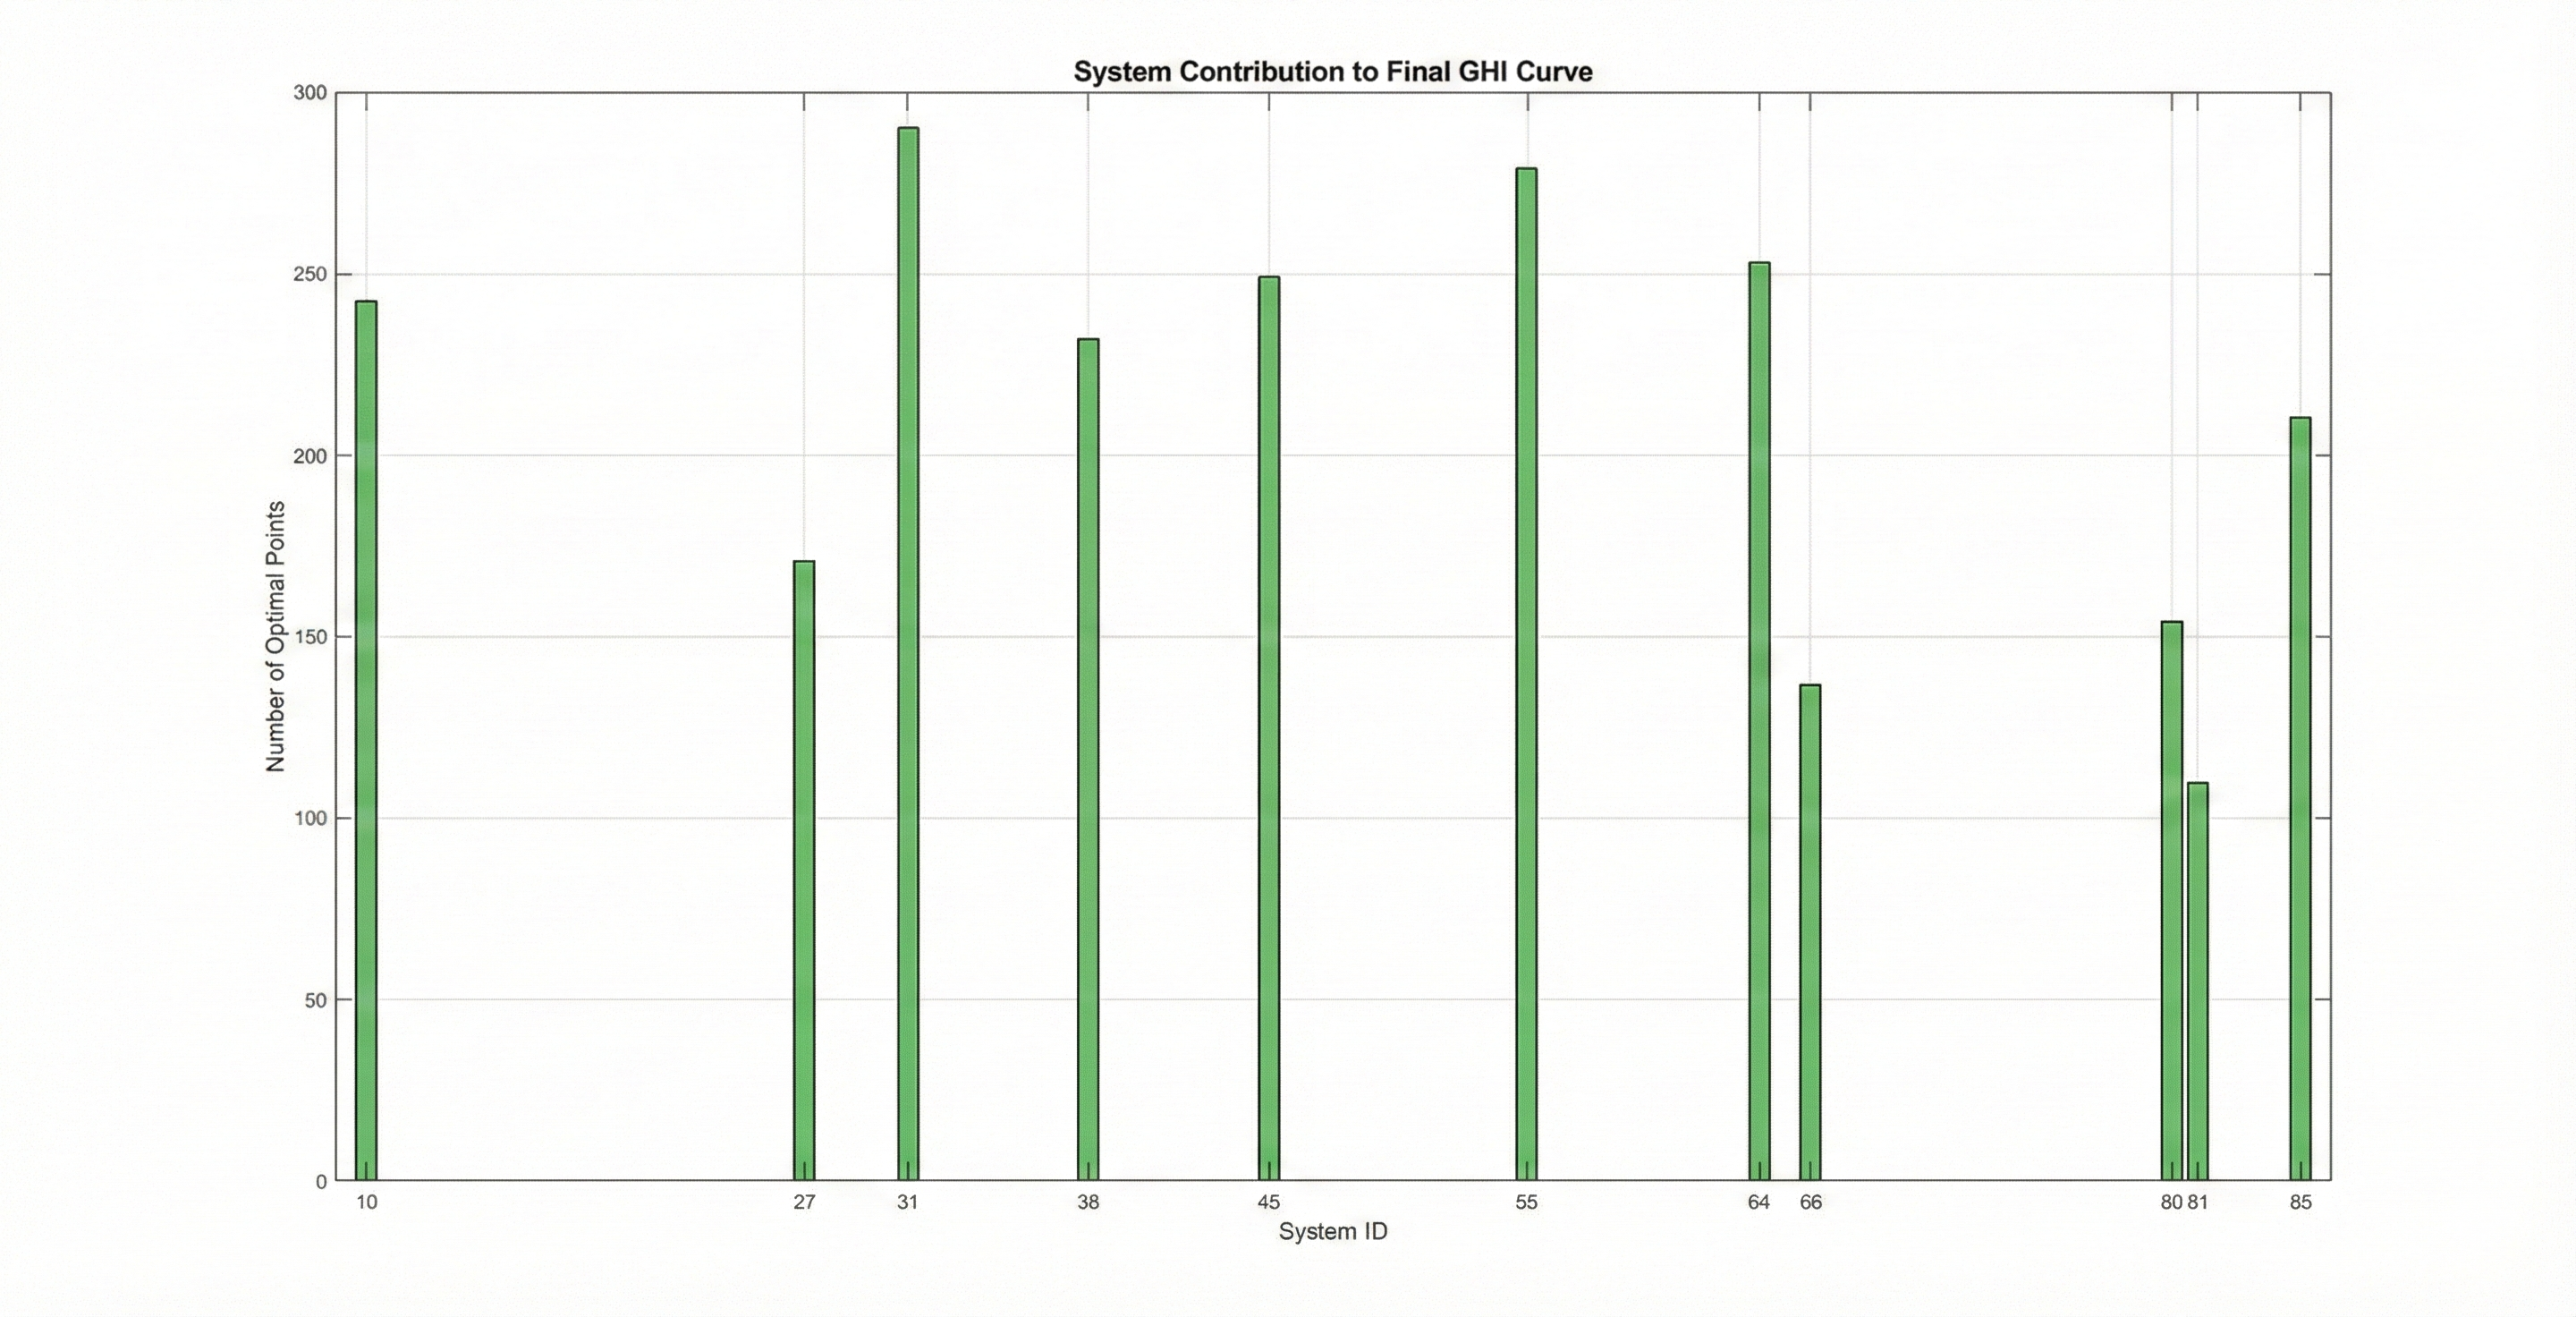
\includegraphics[width=0.8\textwidth]{foto/Ibaraki/SysContribution.png}
    \caption{分散環境下における各システムの最終GHIカーブへの貢献度}
    \label{fig:分散環境下における各システムの最終GHIカーブへの貢献度}
\end{figure}

\textbf{長期的安定性とドリフトの抑制}

図\ref{fig:週間平均誤差の時系列トレンド}に、年間を通じた週間平均誤差の時系列トレンドを示す。

緑色のトレンドラインの傾きは **$-0.335$** であり、Dataset A(傾き -0.090)と比較すると若干の低下傾向(負のドリフト)が見られるものの、年間を通じた変動としては許容範囲内に留まっている。

ごとの変動幅が大きいのは、前項で述べた地理的な不一致や衛星データの誤差に起因する不可避なものであるが、トレンドライン自体が大きく崩れていない点は重要である。これは、温度計なしで $L_{sys}$ に熱損失を吸収させるという簡略化モデルを採用しても、システム的なエラーを招くことなく、年間を通じて一定の推定品質を維持し続けられることを示している。

以上の検証により、提案手法は「データの不完全性」と「地理的な不確実性」という二重の課題を抱える実環境においても、統計的な補正と群知能的な統合によって実用レベルのロバスト性を発揮できることが確認された。

\begin{figure}[htbp]
    \centering
    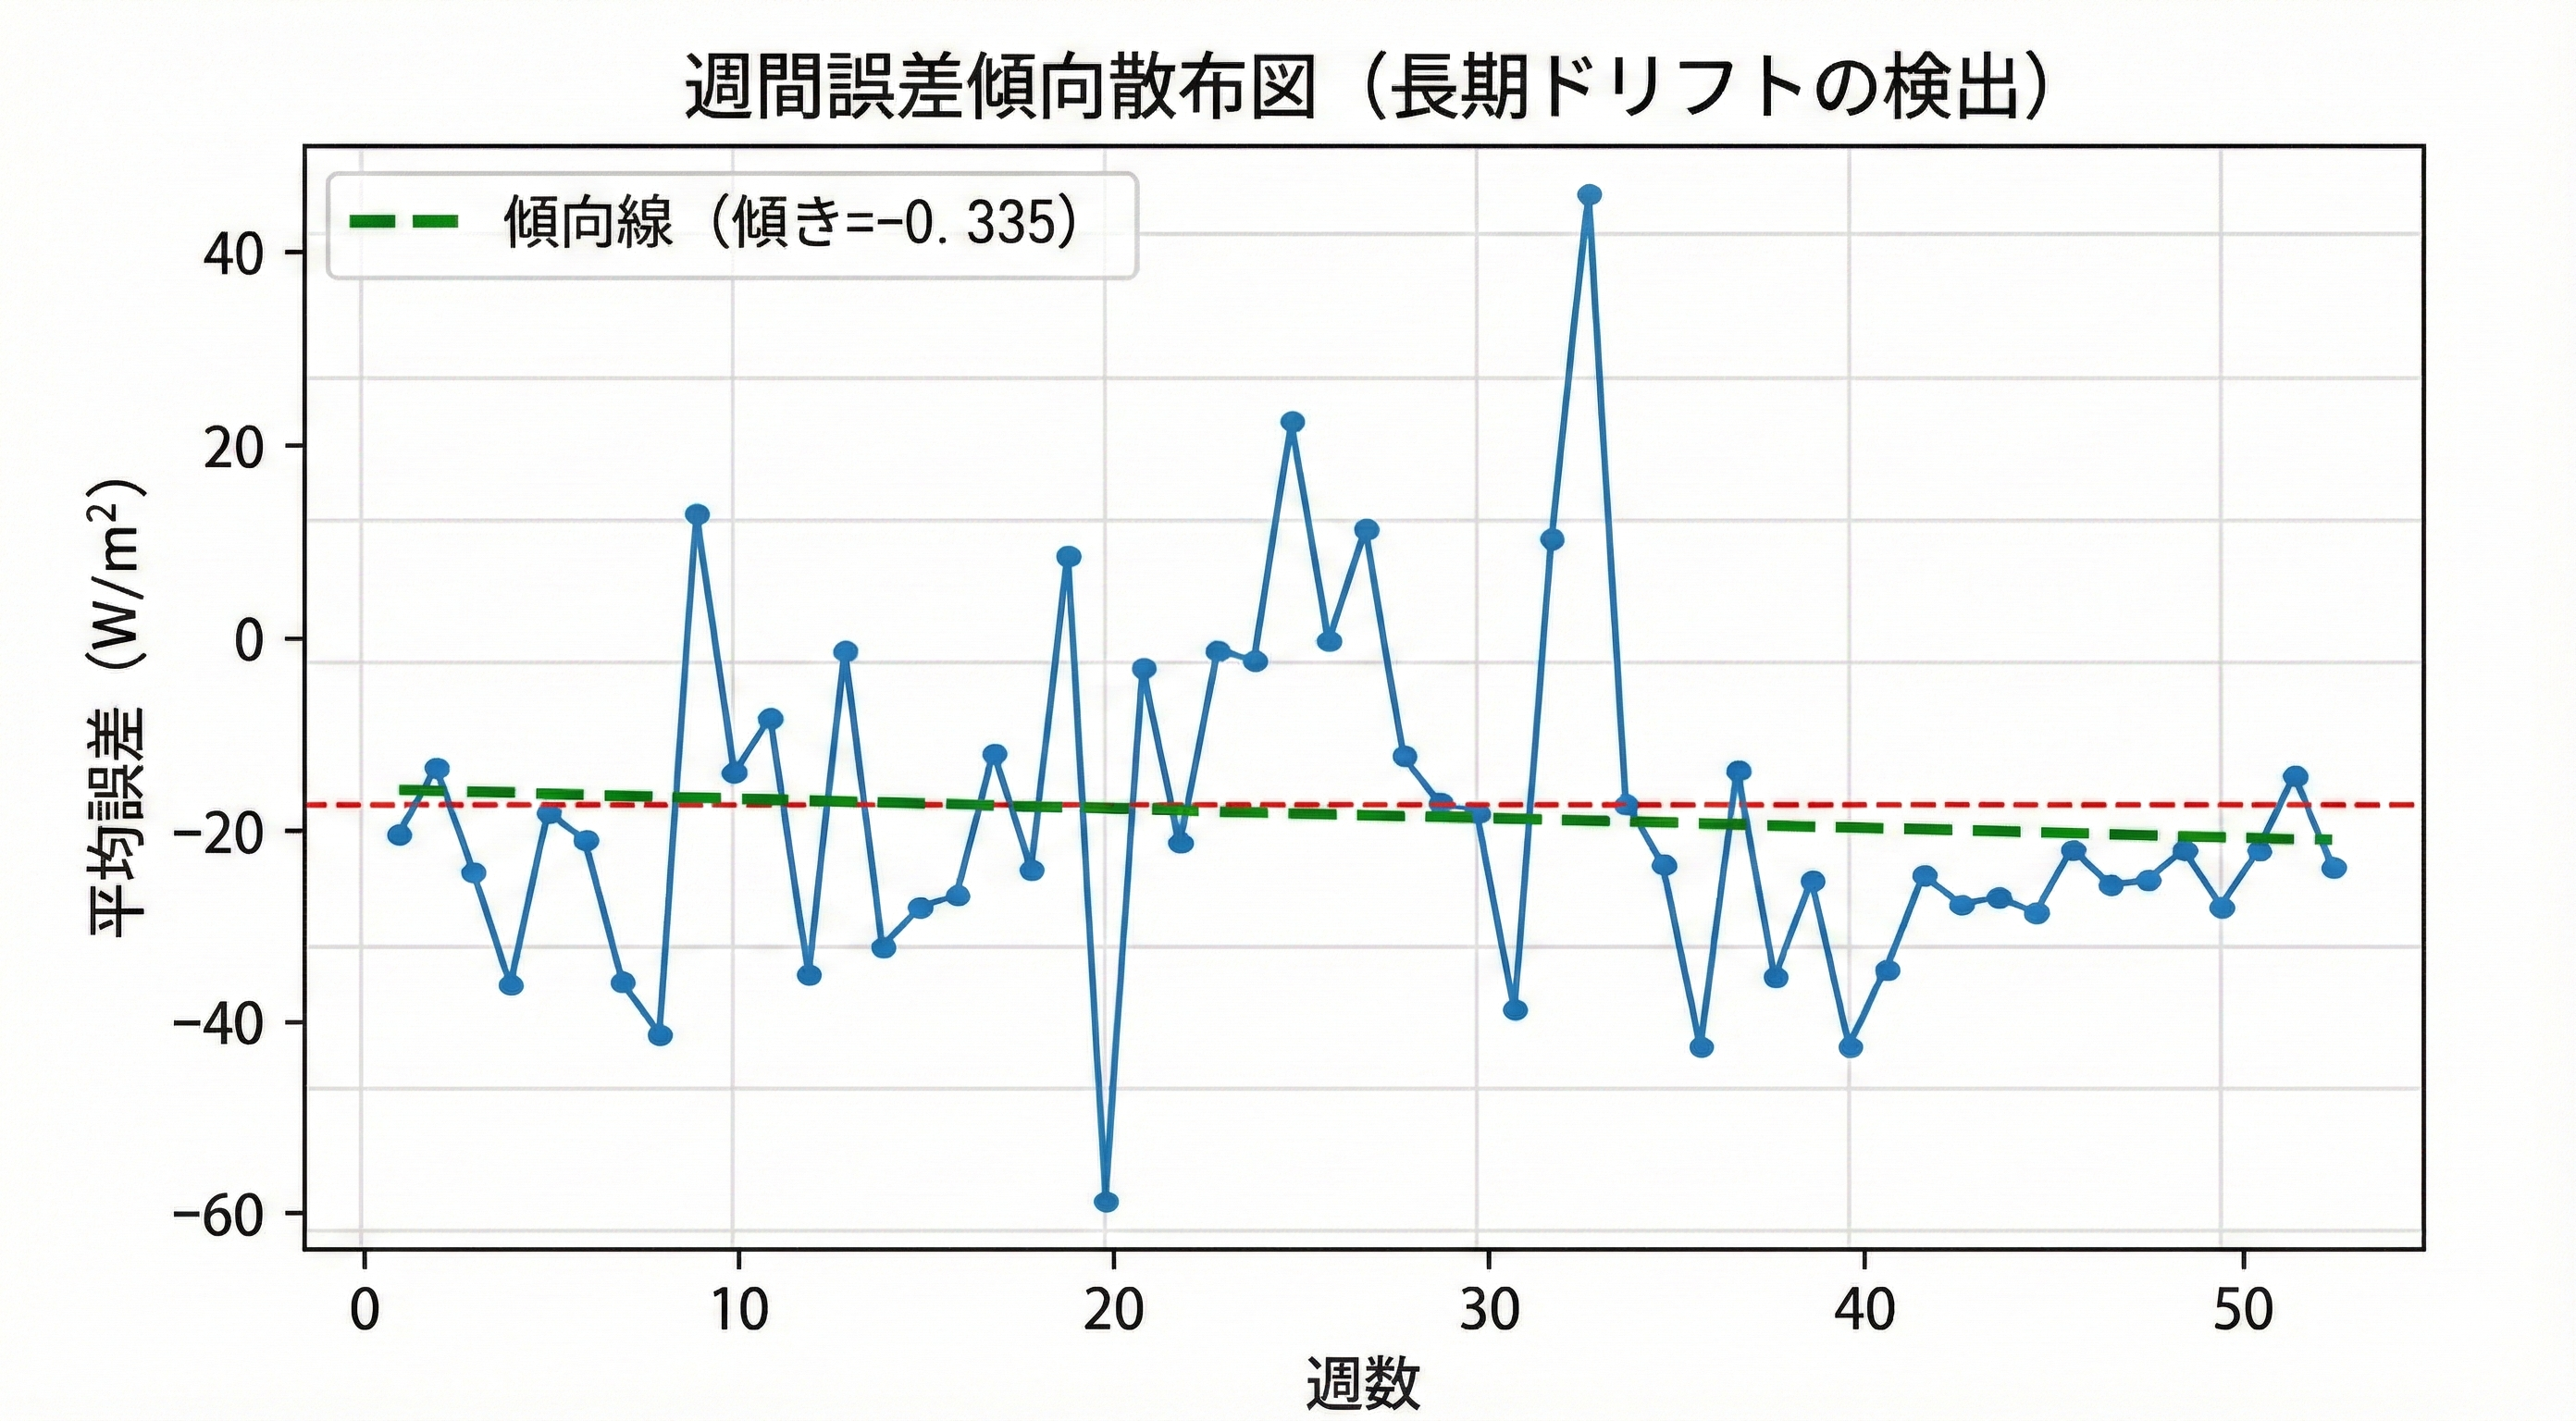
\includegraphics[width=0.8\textwidth]{foto/Ibaraki/ErrorTrendInDifferentWeek.png}
    \caption{週間平均誤差の時系列トレンド(傾き -0.335)}
    \label{fig:週間平均誤差の時系列トレンド}
\end{figure}

%========================================================================
% 第5章 考察 (Chapter 5: Discussion)
% ★ここに考察を記述してください
%========================================================================
\chapter{結論 (Conclusion)}

%************************************************************************
\section{本研究の総括}
%************************************************************************



%************************************************************************
\section{今後の展望}
%************************************************************************



%========================================================================
% 謝辞 (Acknowledgments)
% ★ここに謝辞を記述してください
%========================================================================
\chapter*{謝辞 (Acknowledgments)}
\addcontentsline{toc}{chapter}{謝辞}


本研究を進めるにあたり、終始懇切丁寧なご指導を賜りました〇〇教授に深く感謝いたします。
また、日頃から有益な議論をしていただいた研究室の皆様に感謝いたします。

% 記述例:
% - 指導教員への感謝
% - 副指導教員や共同研究者への感謝
% - 研究室メンバーへの感謝
% - 実験協力者への感謝
% - 家族への感謝


%========================================================================
% 参考文献 (References)
% ★引用した文献を記述してください
%========================================================================
\clearpage

% 1. 设置参考文献列表的标题名称
\addcontentsline{toc}{chapter}{参考文献}

%--- 手動で書く場合 ---
\begin{thebibliography}{99}

    \bibitem{ref1}
    IPCC: Climate Change 2023: Synthesis Report. Contribution of Working Groups I, II and III to the Sixth Assessment Report of the Intergovernmental Panel on Climate Change [Core Writing Team, H. Lee and J. Romero (eds.)]. IPCC, Geneva, Switzerland, 2023.

    \bibitem{ref2}
    環境省: 地球温暖化対策計画(令和3年10月22日閣議決定), 2021.

    \bibitem{ref3}
    経済産業省 資源エネルギー庁: 令和5年度エネルギーに関する年次報告(エネルギー白書2024), 2024.

    \bibitem{ref4}
    経済産業省: 第6次エネルギー基本計画, 2021.

    \bibitem{ref5}
    経済産業省 調達価格等算定委員会: 令和6年度以降の調達価格等に関する意見, 2024.

    \bibitem{ref6}
    JIS C8960,太陽光発電用語,2012.

    \bibitem{ref7}
    株式会社気象データシステム.“技術資料:天文的パラメータ及び日射状況を表す指標の算出方法”.2020


\end{thebibliography}
\end{document}
